\documentclass[11pt,oneside,chapters]{starlink}

\usepackage{amsfonts}

\stardoccategory    {Starlink Cookbook}
\stardocinitials    {SC}
\stardocsource      {sc\stardocnumber}
\stardoccopyright   {Copyright \copyright\ 2015-2018 Science and Technology Facilities Council,\\
                    \& East Asian Observatory}
\stardocnumber      {20.2}
\stardocauthors     {H.\ S.\ Thomas, Malcolm J.\ Currie, \& H.\ A.\ L.\ Parsons}
\stardocdate        {2020 November 4}
\stardoctitle       {The Heterodyne Data Reduction Cookbook}
\stardocversion     {1.2}
\stardocmanual      {\ }
\stardocabstract    {
      This cookbook provides a short introduction to Starlink
      facilities, especially \smurf---the Sub-Millimetre User
      Reduction Facility---and \Kappa---the Kernel Application
      Package---for reducing, displaying, and analysing ACSIS data. In
      particular, this cookbook illustrates the various steps required
      to reduce the data; and gives an overview of the ORAC-DR
      pipeline which carries out many of these steps using a single
      command. Specialised pipeline recipes are discussed.
      The cookbook also introduces cube analysis with the \gaia\
      display tool, and spectral analysis with \splat.}

%-------------------------------------------------------------------

% Local Definitions
\providecommand{\lutedit}{\xref{\task{lutedit}}{sun95}{LUTEDIT}}
\providecommand{\broadline}{\xref{REDUCE\_SCIENCE\_BROADLINE}{sun260}{REDUCE_SCIENCE_BROADLINE}}
\providecommand{\gradient}{\xref{REDUCE\_SCIENCE\_GRADIENT}{sun260}{REDUCE_SCIENCE_GRADIENT}}
\providecommand{\narrowline}{\xref{REDUCE\_SCIENCE\_NARROWLINE}{sun260}{REDUCE_SCIENCE_NARROWLINE}}
\providecommand{\lineforest}{\xref{REDUCE\_SCIENCE\_LINEFOREST}{sun260}{REDUCE_SCIENCE_LINEFOREST}}
\providecommand{\continuum}{\xref{REDUCE\_SCIENCE\_CONTINUUM}{sun260}{REDUCE_SCIENCE_CONTINUUM}}
\providecommand{\calibratesideband}{\xref{CALIBRATE\_SIDEBAND\_RATIO}{sun265}{CALIBRATE_SIDEBAND_RATIO}}

\newcommand{\acsispipelinesun}{\xref{\textbf{SUN/260}}{sun260}{}}

\providecommand{\gaiasc}{\xref{\textbf{SC/17}}{sc17}{}}
\providecommand{\splatsun}{\xref{\textbf{SUN/243}}{sun243}{}}

\providecommand{\cadd}{\xref{\task{cadd}}{sun95}{CADD}}
\providecommand{\chanmap}{\xref{\task{chanmap}}{sun95}{CHANMAP}}
\providecommand{\contour}{\xref{\task{contour}}{sun95}{CONTOUR}}
\providecommand{\gdstate}{\xref{\task{gdstate}}{sun95}{GDSTATE}}
\providecommand{\mfittrend}{\xref{\task{mfittrend}}{sun95}{MFITTREND}}
\providecommand{\nomagic}{\xref{\task{nomagic}}{sun95}{NOMAGIC}}
\providecommand{\sqorst}{\xref{\task{sqorst}}{sun95}{SQORST}}

% Frame attributes fount.
\providecommand{\att}[1]{\textsf{#1}}

% degrees, arcminutes, arcseconds symbols
%\usepackage{siunitx}
\ifpdf
%  \newcommand{\dgs}{\si{\degree}}%$^{\circ}$}
  \newcommand{\udeg}{\hspace{-0.3em}\dgs\hspace{-0.08em}}
%  \newcommand{\arcm}{\si{\arcminute}}%\hbox{$^{\prime$}}}
%  \newcommand{\arcsec}{\si{\arcsecond}}%\arcm\hspace{-0.1em}\arcm}
  \newcommand{\uarcs}{\hspace{-0.27em}\arcsec\hspace{-0.07em}}
  \newcommand{\kms}{\mbox{$\,$km~s$^{-1}$}}   % km/s

\else
%  \newcommand{\dgs}{\HCode{&deg}}
  \newcommand{\udeg}{\HCode{&deg}}
%   \newcommand{\arcm}{$'$}
%   \newcommand{\arcsec}{$''$}
   \newcommand{\uarcs}{$''$}
   \newcommand{\kms}{\,km~s$^{-1}$}   % km/s
\fi

\newcommand{\trs}{$T_{\textnormal{R}}^{*}$}

% arcminute symbol

% arcsec symbol

% decimal-degree symbol

% decimal-arcsecond symbol

%-------------------------------------------------------------------

\begin{document}
\scfrontmatter

% Acronyms section
\Acronyms

\begin{table}[h!]
\begin{tabular}{ll}
\textbf{ACSIS}& Auto-Correlation Spectrometer and Imaging System\\
\textbf{ARD}& ASCII Region Definition\\
\textbf{CADC}& Canadian Astronomy Data Centre\\
\textbf{CSO}& Caltech Submillimetre Observatory\\
\textbf{FITS}& Flexible Image Transport System\\
\textbf{FWHM}& Full-Width at Half-Maximum\\
\textbf{GAIA}& Graphical Astronomy and Image Analysis Tool\\
\textbf{HDS}& Hierarchical Data System\\
\textbf{JCMT}& James Clerk Maxwell Telescope\\
\textbf{LSB}& Lower sideband\\
\textbf{MSB}& Minimum Schedulable Block\\
\textbf{NDF}& Extensible $N$-Dimensional Data Format\\
\textbf{HARP}& Heterodyne Array Receiver Programme\\
\textbf{QA}& Quality Assurance\\
\textbf{RxA}& Receiver A\\
\textbf{SAMP}& Simple Application Messaging Protocol\\
\textbf{SDF}& Starlink Data File\\
\textbf{S/N}& Signal-to-Noise ratio\\
\textbf{USB}& Upper sideband\\
\textbf{WCS}& World Co-ordinate System\\
\textbf{WVM}& Water Vapour radioMeter\\
\end{tabular}
\end{table}


\chapter{\xlabel{introduction}Introduction}
\label{sec:intro}

\section{\xlabel{using_guide}This cookbook}
This cookbook is designed to instruct ACSIS users on the best ways to
reduce and visualise their data using \starlink\ packages.

This guide covers the following:
\begin{itemize}
\itemsep0em
\item \cref{Chapter}{sec:intro}{Chapter 1} -- Computer resources and software you'll need before getting started.
\item \cref{Chapter}{sec:starlink}{Chapter 2} -- Starlink basics---tools for exploring your data.
\item \cref{Chapter}{sec:het}{Chapter 3} -- Heterodyne observing at the JCMT.
\item \cref{Chapter}{sec:raw}{Chapter 4} -- Naming convention and examining raw ACSIS data.
\item \cref{Chapter}{sec:pipe}{Chapter 5} -- The ACSIS pipeline and recipes explained.
\item \cref{Chapter}{sec:runpipe}{Chapter 6} -- How to run the pipeline.
\item \cref{Chapter}{sec:reduce}{Chapter 7} -- Regridding your data with \makecube.
\item \cref{Chapter}{sec:analyse}{Chapter 8} -- Analysing your reduced cube.
\item \cref{Chapter}{sec:advanced}{Chapter 9} -- Advanced analysis techniques such as changing co-ordinate frames.
\item \cref{Chapter}{sec:gaia}{Chapter 10} -- Using \gaia\ to analyse your data.
\item \cref{Chapter}{sec:fromcadc}{Chapter 11} -- Getting your data from CADC.
\end{itemize}

\textbf{Style convention}\\
In this cookbook the following styles are followed:
\begin{itemize}[noitemsep,nolistsep]
\item \texttt{\%} represents the command-line prompt.
\item Command-line examples are shown in \texttt{\color{MidnightBlue}{navy typewriter font.}}
\item Parameters, FITS keywords, parameters and their values are presented in \texttt{typewriter font}.
\item The names of Starlink commands appear as in \task{san serif font}.
\item The names of commands, menu items, tabs, or buttons within graphical tools (such as \gaia\ or
\splat) appear \guithing{like this}.
\item The names of windows produced by graphical tools appear \guiwindow{like this}.
\item The names of attributes appear like \att{StdOfRest}.
\item Useful tips or reminders are given in outlined boxes.
\end{itemize}

\section{\xlabel{computing} Before you start: computing resources}
\label{sec:computing}

Before reducing heterodyne data you should consider whether you have
sufficient computing resources for your data.  That said, there can
only be vague guidelines because resource usage depends on many
factors, such as the spatial area and resolution, the number of
observations being reduced together, observing and bandwidth modes
(see \cref{Section}{sec:obsmodes}{Observing modes}), and the number of
subbands.  However, the main factor is the volume of data being
processed concurrently.

The \oracdr\ \cite{oracdr,oracdr_infra} pipeline can demand approaching
300~GB of peak storage for the largest (about a degree square) HARP maps,
and at least 24~GB of memory during spectral-cube creation.  For
more-normal-sized maps of individual targets, say 20 square arcminutes
from your observations, would only require about 10~GB of storage and
most modern computers would have sufficient memory.  The storage
requirements can more than double if all intermediate files are
retained for diagnostic purposes; intermediate files are normally
removed at the end of each pass through a recipe.  Reducing manually
permits you to tidy files as you move along, but is very time consuming.

Reducing RxA data and HARP stares or small jiggle maps is
undemanding of resources.

\section{\xlabel{software}Before you start: Starlink software}

This manual utilises software from the \starlink\ package; \smurf\
\cite{smurf}, \Kappa\ \cite{kappa}, \gaia\ \cite{gaia}, \oracdr\
\cite{oracdr}, \convert\ \cite{convert}, \cupid\ \cite{cupid},
\ccdpack\ \cite{ccdpack}, and
\picard\ \cite{picard}. Starlink software must be installed on your
system, and Starlink aliases and environment variables must be defined
before attempting any ACSIS data reduction. You can download Starlink
from  \htmladdnormallink{the Starlink webpage}{http://www.starlink.ac.uk}.

Below is a brief summary of the packages used in this cookbook and how
to initialise them. Note that all the example commands are shown within
a UNIX shell.

\begin{table}[h!]
\begin{tabular}{p{1.7cm}|p{7.4cm}|p{2.9cm}|p{2.2cm}}

\textbf{Package} & \textbf{Description} & \textbf{Initialise}  & \textbf{Help}\\
\hline
\smurf\ & The Sub-Millimetre User Reduction Facility (\smurf) contains
          \makecube\ that will process raw ACSIS data into spectral cubes.
        &  \texttt{\%\,smurf} & \texttt{\%\,smurfhelp} \newline \smurfsun\\
\hline
\Kappa\ & A general-purpose applications package with commands for
          processing, visualising, and manipulating NDFs. & \texttt{\%\,kappa}
        & \texttt{\%\,kaphelp} \newline \kappasun\ \\
\hline
\convert\ & CONVERT allows the interchange of data files to and from
            NDF. Other formats include IRAF, FITS, and ASCII.
          & \texttt{\%\,convert} & \texttt{\%\,conhelp} \newline \convertsun\ \\
\hline
\cupid\ & CUPID is a package of commands that allows the identification
          and analysis of clumps of emission within one-, two- or
          three-dimensional data arrays & \texttt{\%\,cupid}
        & \texttt{\%\,cupidhelp} \newline \cupidsun\ \\
\hline
\oracdr\ & The \ORACDR\ Data Reduction Pipeline \cite{oracdr} is an
           automated reduction pipeline. \ORACDR\ uses \smurf\ and
           \Kappa\ (along with other Starlink tools) to perform an automated
           reduction of the raw data following pre-defined recipes.
         & \texttt{\%\,oracdr\_acsis} & \oracdrsun \\
\hline
\textsc{Picard} & \textsc{Picard} uses a similar pipeline system as \ORACDR\ but
                  for the post-processing of reduced data. While mainly implemented
                  for SCUBA-2 data, there are a few recipes that are heterodyne
                  compatible. See \cref{Appendix}{app:picard}{Picard} for more details
                  and a description of the available recipes.
                & \texttt{\%\,picard RECIPE $<$files$>$} & \picardsun\ \\
\hline
\multicolumn{4}{l}{}\\
\textbf{Tool} & \textbf{Description} & \textbf{Open}  & \textbf{Help}\\
\hline
\gaia\ & \gaia\ is an interactive image and data-cube display and
         analysis tool. It incorporates tools such as source detection,
         three-dimensional visualisation, clump visualisation, photometry,
         and the ability to query and overlay on-line or local catalogues.
       & \texttt{\%\,gaia} & \gaiasun\ \gaiasc\ \\

\hline
\HDSTRACE\ & This tool lets you examine the contents of Starlink data files.
           & \texttt{\%\,hdstrace $<$file$>$} & \hdstracesun\ \\

\hline
\splat\ & \splat\ is a graphical spectral-analysis tool. It can also
           interact with the Virtual Observatory.  & \texttt{\%\,splat}
        & \splatsun\ \\
\hline
\end{tabular}
\end{table}

\section{\xlabel{software_options}Options for Reducing your Data}

You have three options for processing your data:
\\\\
(1) performing each step manually,\\
(2) write your own scripts, or \\
(3) running the automated pipeline.
\\\\
\emph{The automated pipeline is recommended for new users of JCMT
heterodyne data or those unfamiliar with the Starlink software.}
The pipeline approach works well if your project is suited to using
one of the standard recipes, as are most projects.  Running the pipeline
is probably essential if you have a lot of data to process.
To use the science pipeline, skip straight to
\cref{Chapter}{sec:pipe}{The ACSIS Pipeline}.

Performing each step by hand allows more fine-tuned control of certain
processing and analysis steps, although some fine-tuning is available
in the pipeline via recipe parameters (see
\cref{Section}{sec:recpars}{Recipe parameters}).

Once you have determined your optimal parameters you can pass them to
the pipeline or a script. \cref{Chapter}{sec:reduce}{Regridding your
Data} and \cref{Chapter}{sec:analyse}{Analysing your Cube} discuss the
manual approach.

While you have the option of running the pipeline yourself, you can
find pipeline reduced files for individual and co-added observations by
night in the \htmladdnormallink{JCMT Science
Archive}{http://www3.cadc-ccda.hia-iha.nrc-cnrc.gc.ca/jcmt/} (JSA).

These have been reduced using the \ORACDR\ pipeline with the recipe
specified in the MSB or with the Legacy Survey recipe.  Principal
investigators (PIs) and co-investigators (co-Is) can access these data
through the JSA before it becomes public by following the instructions
in \cref{Section}{sec:fromcadc}{Getting your data from CADC}.

\newpage
\chapter{\xlabel{starlink}Good to know: Starlink}
\label{sec:starlink}

\section{File format}
\label{sec:format}

Starlink routines run on HDS files (Hierarchical Data System), which
normally have a \file{.sdf} extension (Starlink Data File).
HDS files can describe a multitude of formats. The most common HDS
format you will encounter is the NDF ($N$-Dimensional Data
Format)\cite{ssds}. This is the standard file format for storing data
that represent $N$-dimensional arrays of numbers, such as spectra, and
images.  The parameter files discussed in
\cref{Section}{sec:hdstrace}{How to find the current parameter values}
are also HDS format.

Raw data retrieved from the JCMT Science Archive come in FITS format.
For information on converting between FITS and NDF see
\cref{Appendix}{app:convert}{Converting file formats}.

\begin{tip}
The \file{.sdf} extension of HDS filenames is not required when running
Starlink commands.
\end{tip}

\section{\xlabel{parameters}Parameters}
\label{sec:parameters}

Parameters control the behaviour and data processed in Starlink
applications.  A parameter expects a value that is one of the
following types: string, boolean, integer, or single- or
double-precision floating point.  You can either specify parameter
values on the command line or in response to prompts.  Most parameters
have sensible defaults leaving you to concentrate on the main
parameters.  Parameter usage is described in a
\xref{tutorial}{sun95}{se_param}

\section{\xlabel{adam}How to find the current parameter values}
\label{sec:hdstrace}

A directory called \texttt{adam} is created in your home-space by
default when you run Starlink applications. In this directory you will
find HDS files for each of the application that you have run. These
files contain the parameters used and results returned (if
appropriate) from the last time you ran a particular application.

You can specify a different location for the \texttt{adam} directory
by setting the environment variable \texttt{ADAM\_USER} to be the path
to your alternative location. This is useful when running more than
one reduction to avoid interference or access clashes.

To see the ADAM parameters, run \HDSTRACE\ on any of the parameter
files. For example, to see which parameters were used and the results
from last time you ran \stats, you can type the following from
anywhere on your system:

\begin{terminalv}
% hdstrace ~/adam/stats
\end{terminalv}

This will report the following
\begin{terminalv}
STATS  <STRUC>
   ADAM_DYNDEF    <DEFAULTS>      {structure}
   COMP           <_CHAR*132>     'DATA'
   ORDER          <_LOGICAL>      TRUE
   MAXIMUM        <_DOUBLE>       36.666870117188
   MAXWCS         <_CHAR*132>     '10.625136, -0.381122, -6.057133'
   MINWCS         <_CHAR*132>     '10.720136, -0.017795, -31.05713'
   MEAN           <_DOUBLE>       0.25890738014562
   MINIMUM        <_DOUBLE>       -2.7510244846344
   SIGMA          <_DOUBLE>       0.72429928153974
    ..               ..                 ..
    ..               ..                 ..
\end{terminalv}
\vspace{0.3cm}
You can see \stats\ was run on the data array with ordered statistics
as well as the resulting values. Any of the parameters returned by
running \HDSTRACE\ on an ADAM file can be extracted using the command
\task{parget}. In the example below, the mean value from the last
instance of \task{stats} is printed to the screen.
\begin{terminalv}
% parget mean stats
\end{terminalv}

\begin{tip}
Try not to exit from Starlink tasks by breaking in, since this may
corrupt the parameter file (reported as an integrity check error).  If
this happens delete the parameter file.  Enter \texttt{!!} at a prompt
if possible to have a clean exit.
\end{tip}

\subsection{Extracting a value for scripting}

\parget\ is designed to make life easier when passing values between
shell scripts. In the C-shell scripting example below, the median
value from \task{histat} is assigned to the variable med.  Note the
use of the back quotes.

For more information on scripting our work see
\cref{Appendix}{app:script}{Scripting your reduction}.

\begin{terminalv}
set med = `parget median histat`
\end{terminalv}

If the parameter comprises a vector of values these can be stored in a
C-shell array. For other scripting languages such as Python, the
alternative vector format produced by setting parameter VECTOR to TRUE
may be more appropriate. Single elements of a parameter array may also
be accessed using the array index in parentheses.

In addition to running \task{hdstrace} on the ADAM file, you can find
a list of all parameter names that can be returned with \parget\ in
the \xref{\textsc{Kappa} manual}{sun95}{} under `Results Parameters'
for the command in question. Note that these names may be different
from the names returned in a terminal when running application.

\section{How can I view the metadata?}
\label{sec:fitslist}

There are two \Kappa\ tasks which are extremely useful for examining
your metadata: \fitslist\ and \ndftrace, which can be used to view the
FITS headers and properties, such as dimensions, of the data
respectively. The third option is the stand-alone application
\HDSTRACE.
\vspace{0.7cm}\\
\begin{aligndesc}
\item[\textbf{fitslist}]
This lists the FITS header information
for any NDF (raw or reduced). This extensive list includes dates \&
times, source name, observation type, band width, number of channels,
receptor information, exposure time, start and end elevation and
opacity. In the example below, just the object name is extracted.
\begin{terminalv}
% fitslist file | grep OBJECT
\end{terminalv}
Likewise, if you know the name of the keyword you want to view, you can
use the \fitsval\ command instead, for instance
\begin{terminalv}
% fitsval file OBJECT
\end{terminalv}

\item[\textbf{ndftrace}]
\task{ndftrace} displays the attributes of the NDF data structure.
This will tell you, for example, the units of the data, pixel bounds,
dimensions, world co-ordinates (WCS), and axis assignations.
\begin{terminalv}
% ndftrace map fullframe fullwcs
\end{terminalv}

An NDF can contain more than one set of world co-ordinates. The
\param{fullwcs} parameter requests that all sets be listed rather
than the currently chosen one.

\item[\textbf{hdstrace}]
\task{hdstrace} lists the name, data type and values of an HDS
(Hierarchical Data System) object. The following example shows the
structure of a time-series cube, including the pixel origin of the
data structure. To show just the first $x$ lines of values for each
parameter include the option \param{nlines=x} on the command line:
\begin{terminalv}
% hdstrace file nlines=3
\end{terminalv}
Otherwise to see all the lines and information that is available in
each extension use \param{nlines=all}. The example below displays all
the system temperature values and pipes the result to `less' to make
viewing easier.
\begin{terminalv}
% hdstrace file.MORE.ACSIS.TSYS nlines=all | less
\end{terminalv}
\end{aligndesc}
\vspace{0.4cm}

You can see it descends two levels (into \texttt{MORE} and
\texttt{ACSIS}) to retrieve the information. Other information
available at this level include receptors and receiver temperatures.

Full details of \ndftrace\ and \fitslist\ can be found in the
\xref{\textsc{Kappa} manual}{sun95}{}. Details on \HDSTRACE\ can be
found in the \xref{\textsc{hdstrace} manual}{sun102}{}.



\section{What has already been done to the data?}

If you are presented with a data file you may wish to see what
commands have been run on it and, in the case of a co-added cube, which
data went into it. Two \Kappa\ commands can help you with this:
\vspace{0.7cm}\\
\begin{aligndesc}
\item[\textbf{hislist}]
The \Kappa\ command \hislist\ will return the history records of the NDF.
\begin{terminalv}
% hislist myfile brief
\end{terminalv}
Including the \param{brief} option returns a simple list of the
commands. Omitting this will include the text associated with each
command and can be useful for finding out what parameters were used in
each case. This works for all NDFs including those reduced by the
pipeline, for these all the commands executed as part of the pipeline
reduction script will be listed. The version of software used for each
step is also reported.

\item[\textbf{provshow}]
The \Kappa\ command \task{provshow} displays the details of the NDFs
that were used in the creation of the given file. It includes both
immediate parents and older ancestor NDFs.
\begin{terminalv}
% provshow file
\end{terminalv}
\end{aligndesc}

\section{\xlabel{ndfsections}How to examine, process or extract a subset of your data}
\label{sec:ndfsections}

For all Starlink commands you can specify a sub-section of your data
on which to run an application. You do this by appending the bounds of
the section to be processed the NDF name. This may be on the command
line or in response to a prompt.

The example below runs \stats\ on a sub-cube within your original
cube. This sub-cube is defined by bounds given for each axis. The
upper and lower bounds for each axis are separated by a colon, while
the axes themselves are separated by a comma. Note that the use of
quotes is necessary on a UNIX shell command line, but not in response
to a prompt or in many other scripting languages.

\begin{terminalv}
% stats `cube(10.5:10.0,0.0:0.25,-25.:25.)'
\end{terminalv}
The bounds are given in the co-ordinates of the data (Galactic for Axes
1 and 2 and velocity for Axis 3). You can find the number and names of
the axes along with the pixel bounds of your data file by running
\ndftrace. In the example above the ranges are 10.5$^\circ$ to
10$^\circ$ in Longitude (note the range goes from left to right),
0$^\circ$ to 0.25$^\circ$ in Latitude, and -25 to +25\kms\ in
velocity. To leave an axis untouched simply include the comma but do
not specify any bounds.


\begin{tip}
Be careful to give world co-ordinate values in floating point.
Integers are interpreted as pixel indices.
\end{tip}

To define your bounds in FK5 co-ordinates use the following format.
\begin{terminalv}
% stats `cube(22h18m:22h32m,05d:05d30m,)'
\end{terminalv}

To write a section of your data into a new file (called
\file{newcube.sdf} in the example below) use \ndfcopy\ with bounds.
\begin{terminalv}
% ndfcopy `cube(10.5:10.0,0.0:0.25,-25:25)' newcube title='"l=10.5 sub-section"'
\end{terminalv}
Here the option \param{title} defines a title for the new cube which
replaces the title derived from the original.

You can also define a region as a number of pixels from a given
origin. The example below extracts a 25$\times$25 pixels cube around
the position $l=10^\circ$, $b=0^\circ$.
\begin{terminalv}
% ndfcopy `cube(10.0~25:0.0~25,)' newcube
\end{terminalv}

\begin{tip}
To help identify your sub-region in pixel co-ordinates, open your
file in \gaia\ and change the built-in co-ordinates to PIXEL via
\guithing{Image-Analysis} $>$ \guithing{Change coordinate} $>$
\guithing{Built-in coordinates}.
\end{tip}


\newpage
\section{\xlabel{help}How to get help}
\label{sec:help}
\begin{table}[h!]
\begin{tabular}{p{2.3cm}|p{7.3cm}|p{5cm}}
\textbf{Command} & \textbf{Description} & \textbf{Usage}\\
\hline
\task{showme} & If you know the name of the Starlink document you want to view,
                use \task{showme}. When run, it launches a new web page or tab
                displaying the hypertext version of the document. &
                \texttt{\% showme sun95}\\
\hline
\task{findme} & \task{findme} searches Starlink documents for a keyword. When
                run, it launches a new web page or tab listing the results. &
                \texttt{\% findme kappa} \newline  \texttt{\% findme heterodyne}\\
\hline
\task{docfind} & \task{docfind} searches the internal list files for keywords. It then
                 searches the document titles. The result is displayed using the
                 UNIX \task{more} command. & \texttt{\% docfind kappa}\\
\hline
Run routines with prompts & You can run any routine with the option
                            \texttt{prompt} after the command. This will
                            prompt for every parameter available. If you
                            then want a further description of any parameter
                            type  \texttt{?} at the relevant prompt. &
                            \texttt{\% makemap prompt \newline\ \% REF - Ref. NDF /!/$>$ ?}\\
\hline
\end{tabular}
\end{table}


\clearpage
\chapter{\xlabel{het_overview}JCMT Heterodyne Observing}
\label{sec:het}

\section{\xlabel{specline}Spectral-line Observing}

Submillimetre instruments use heterodyne techniques to observe
spectral lines at high resolution. Heterodyne receivers take a weak
incoming signal and mix it with a reference frequency known as the
local oscillator (LO). This results in a signal of lower
(intermediate) frequency (IF) which can be amplified and more easily
sampled. The current JCMT receivers have an IF of 4\,GHz (RxA) or
5\,GHz (HARP). This mixing produces two frequencies for each value of
the LO ($\nu_{\textnormal{sky}} = \nu_{\textnormal{LO}}\pm\nu_{\textnormal{IF}}$) which are known as the
upper sideband (USB) and lower sideband (LSB).

In a single-sideband receiver one of these is suppressed. Double-sideband
receivers have the two frequencies superimposed.

Reducing the noise in the system is crucial to the efficiency of these
receivers. The required integration time is directly proportional to
the total noise in the system given by $T_{\textnormal{sys}}$ via the radiometer
formula

\[T_{\textnormal{A}}^*({\textnormal{rms}}) =
\frac{2\,T_{\textnormal{sys}}\,\kappa}{\sqrt{\Delta\nu\,t}},\]

where the terms are as follows:
\begin{itemize}
\item $\Delta\nu$ is the frequency resolution of each channel.

\item $t$ is the total integration time (time spent integrating on the
source and the reference position).

\item $\kappa$ is the telescope specific backend degradation factor.

\item The factor of 2 is required for position-switch or beam-switch
observations where half the time is spend off source at the reference
position. For frequency switched observations it is 1.414 instead.

\item $T_{\textnormal{sys}}$ is the system temperature in kelvin and
describes the total noise of the system. It includes contributions
from the background sky temperature, the Earth's atmosphere, ground
spillover picked up by the side lobes and the noise from the receiver
itself (known as \trs).  \trs\ can
be determined by measuring the effects on $T_{\textnormal{sys}}$ when
looking at hot and cold loads, where the cold load is black-body
source.

\item $T^*_{\textnormal{A}}({\textnormal{rms}})$ is the rms value of the noise observed
in the spectrum in kelvin.
\end{itemize}


\begin{tip}
Both $T_{\textnormal{sys}}$ and \trs\ are stored in
the raw data files. This information is stored in the .MORE.ACSIS.TSYS
and .MORE.ACSIS.TRX extensions respectively, and can be viewed using
\HDSTRACE\ (see \cref{Section}{sec:fitslist}{How can I view the
metadata?}).
\end{tip}


\section{\xlabel{rxa}Heterodyne Instruments}
\label{sec:instruments}

The heterodyne instruments described below are those currently operational,
soon to be operational or recently retired at the JCMT.
For information on previous instruments see the JCMT web pages.

In the following $\eta_{\textnormal{MB}}$ is the main-beam efficiency and
$\eta_{\textnormal{\,fss}}$ is the forward spillover and scattering efficiency.
For the latest and historical calibrations visit
\htmladdnormallink{ACSIS Beam
Efficiencies}{http://www.eaobservatory.org/jcmt/instrumentation/heterodyne/calibration}.



\subsection{N\=amakanui Frontend}

The N\=amakanui instrument is a spare receiver for the Greenland
Telescope (GLT) on loan for use on the JCMT courtesy of ASIAA.
N\=amakanui contains three inserts: Ala$`$ihi, $`$\=U$`$\=u, and
$`$\=Aweoweo operating around 86, 230, and 345\,GHz. Each of the three
inserts receive dual linear polarizations which are labelled using a
zero-based system: P0, P1. Each insert has a separate optical path and
so only one receiver/frequency range can be used at any one time.

\subsection{$`$\=U$`$\=u Frontend (in commissioning)}

$`$\=U$`$\=u is one of three inserts held within the N\=amakanui
instrument. $`$\=U$`$\=u is a dual linear polarizations Sideband
Separating (2SB) instrument. It operates between 215 and 270.6\,GHz.
It achieved first light on 2019 October 5.  The most-common observing
mode for $`$\=U$`$\=u is stare mode, but $`$\=U$`$\=u is also able to
take jiggle and raster maps.

\begin{table}[h!]
\begin{center}
\begin{tabular}{|p{1.5cm}|p{1.2cm}|p{0.8cm}|p{0.8cm}|}
\hline
Receiver &FWHM & $\eta_{\textnormal{MB}}$ & $\eta_{\textnormal{\,fss}}$\\
\hline
$`$\=U$`$\=u&20\uarcs&0.57 & *\\
\hline
\end{tabular}
\end{center}
\end{table}


\subsection{$`$\=Aweoweo Frontend (in commissioning)}

$`$\=Aweoweo is another of three inserts held within the N\=amakanui
instrument. $`$\=Aweoweo, like $`$\=U$`$\=u, is also a dual linear
polarizations Sideband Separating (2SB) instrument. It operates across
a frequency range that spans between 276 and 371\,GHz. $`$\=Aweoweo
saw first light on 2021 January 14.  Due to its sensitivity
$`$\=Aweoweo's most-common observing mode is stare. For larger areas,
HARP becomes more efficient for jiggle and raster mapping.

\subsection{Ala$`$ihi Frontend (future)}

Ala$`$ihi is the other insert held within the N\=amakanui instrument.
Unlike $`$\=U$`$\=u and $`$\=Aweoweo, Ala$`$ihi is a Single SideBand
(SSB) instrument. It will operate at frequencies around 77 to 88\,GHz
with dual linear polarizations. Its primary function at the JCMT will
be as part of VLBI observations.


\subsection{\xlabel{harp}HARP Frontend}

The Heterodyne Receiver Array Programme (HARP) is a 16-receptor array
arranged on a 4$\times$4 grid \cite{harp}. It operates in the B-band
between 325 and 375 GHz. The receptors are adjacent on the focal plane
but separated on the sky by 30 arcseconds (or approximately twice the
beamwidth). The footprint of the full array is 2 arcminutes.  Note
that not all receptors are operational; historically between 12 and 15
receptors have been available at any given time. The tracking receptor
is chosen to be the best performing of the four internal (2$\times$2)
receptors in the grid.

You can find the number of the tracking receptor and the number of
working receptors in the FITS header values \param{REFRECEP} and
\param{N\_MIX} respectively.

In addition to stare observations with the tracking receptor, the most
common observing modes for HARP are jiggles and raster maps. These
observing modes are described in
\cref{Section}{sec:obsmodes}{Observing modes} and an example image
from each mode is shown in \cref{Figure}{fig:harpmodes}{the figure
below}.

\begin{table}[h!]
\begin{center}
\begin{tabular}{|p{1.5cm}|p{1.2cm}|p{0.8cm}|p{0.8cm}|}
\hline
Receiver &FWHM & $\eta_{\textnormal{MB}}$ & $\eta_{\textnormal{\,fss}}$\\
\hline
HARP&14\arcsec &0.63& 0.88\\
\hline
\end{tabular}
\end{center}
\end{table}

\subsection{RxA3 Frontend (retired June 2018)}

Receiver A3 (RxA3) was a single-element double-sideband receiver. It
operates in the A-band between 211 and 276 GHz. In addition to stare
observations, the most common observing mode for RxA3 was raster
mapping. In 2016 RxA3 was updated to RxA3M. The instrument was retired in 2018.

\begin{table}[h!]
\begin{center}
\begin{tabular}{|p{1.5cm}|p{1.2cm}|p{0.8cm}|p{0.8cm}|}
\hline
Receiver &FWHM & $\eta_{\textnormal{MB}}$ & $\eta_{\textnormal{\,fss}}$\\
\hline
RxA3&19.\uarcs7&0.57 & 0.80\\
\hline
\end{tabular}
\end{center}
\end{table}

RxA3M had an additional calibration step (automatically applied by our
pipelines if you use a version after June 2019) to normalise the flux
levels of observations between the upper and lower sideband. If you
need more control of this in the pipeline, please see the calibration
recipe parameters in \cref{Appendix}{app:params}{Classified Recipe
Parameters}.  The older RxA3 also had some variation in flux levels
between the sidebands, but we do not have a calibration correction for
this.


\begin{figure}[b!]
\begin{center}
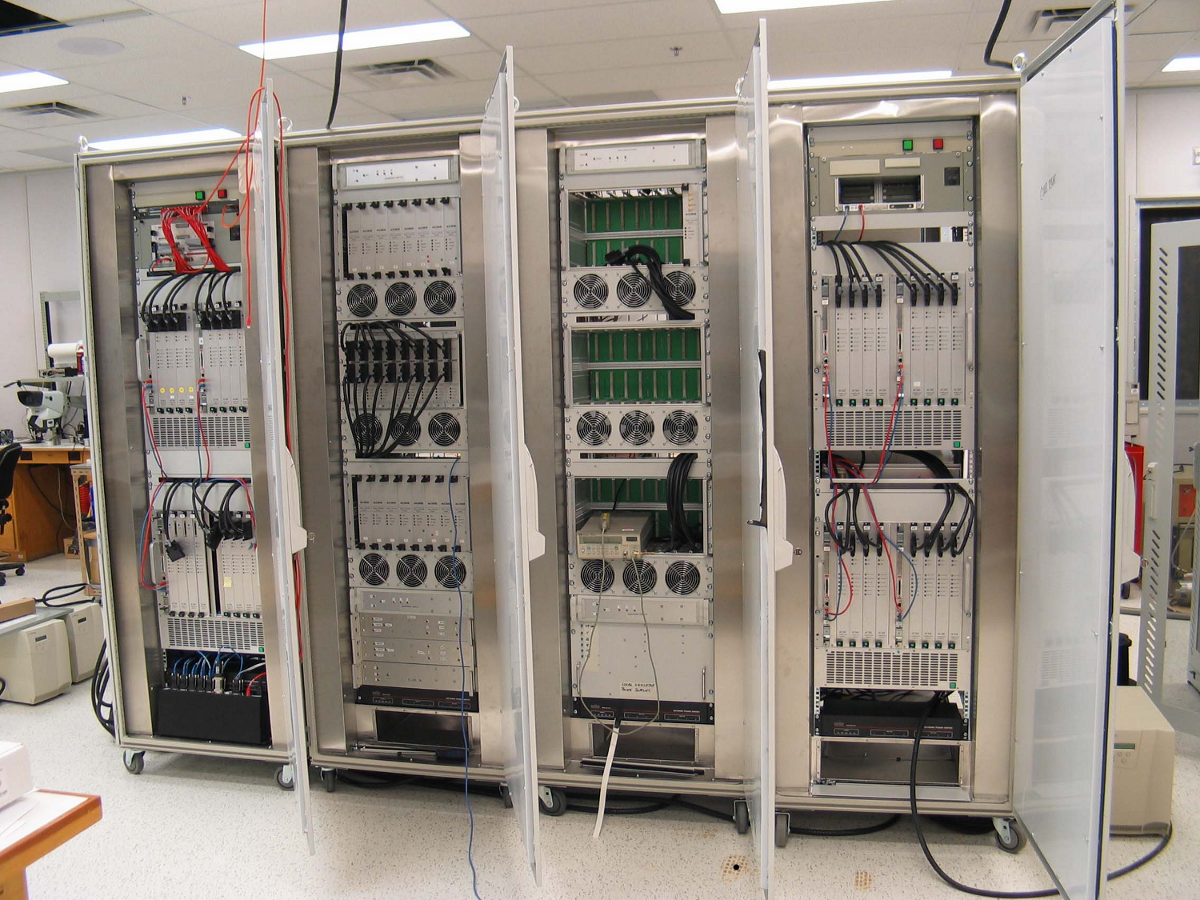
\includegraphics[width=0.7\linewidth]{sc20_acsis_front_sm}
\caption[Front view of ACSIS at the JCMT]{\label{fig:acsis}
  Front view of ACSIS at the JCMT. Although designed to work with HARP,
  ACSIS can be used with any JCMT heterodyne receiver.}
\end{center}
\end{figure}


\subsection{ACSIS Backend}

Since 2006 September, the backend for heterodyne instruments has been the
Auto-Correlation Spectrometer and Imaging System known simply as ACSIS
(see \cref{Figure}{fig:acsis}{}). Given the various combinations of
ACSIS's 32 down-converter modules and available IF outputs from the
different instruments, a number of bandwidth modes and corresponding
frequency resolutions are available. Listed below are the most common
ones. Visit the JCMT web pages for a full list.

\newpage
\begin{table}[h!]
\begin{center}
\begin{tabular}{c|c|c}
\hline
\textbf{Subbands} & \textbf{Bandwidth mode}  & \textbf{Channel Spacing}\\
\hline
1 & 250 MHz & 0.0305 MHz (HARP/RxA/RxW)\\
1 &1000 MHz & 0.488 MHz (HARP/RxA/RxW)\\
1 &1860 MHz (1600,1800) & 0.977 MHz (HARP) \\
  &         & 0.488 MHz (RxA/RxW)\\
1 & 440 MHz (400,420) & 0.061 MHz (HARP) \\
  &         & 0.0305 MHz (RxA/RxW)\\
\hline
2 & any 250 MHz      & 0.061 MHz (HARP)\\
  &         & 0.0305 MHz (RxA/RxW)\\
2 &any 1000 MHz & 0.977 MHz (HARP) \\
  &         & 0.488 MHz (RxA/RxW)\\
\hline
\end{tabular}
\label{fig:backend}
\end{center}
\end{table}
There are a number of special configurations available with ACSIS.
These make use of multiple sub-bands to cover lines at different
frequencies.  You can find the subsystem number for a given
observation by the FITS header \param{SUBSYSNR}.

You will find each subsystem number corresponds to a different
molecule or transition (given by the FITS headers \param{MOLECULE} and
\param{TRANSITI}). The most common pairings are
C$^{18}$O\,(3-2)/$^{13}$CO\,(3-2) and DCN\,(5-4)/HCN\,(4-3) for HARP,
and SiO\,(6$_0$-5$_0$)/SO\,(4$_3$-3$_4$) for RxA.

\begin{figure}[t!]
\begin{center}
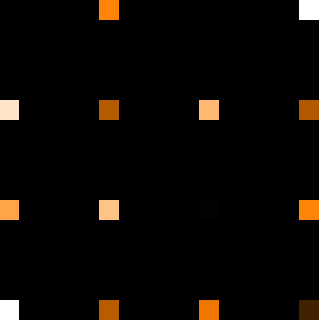
\includegraphics[width=5.2cm, height=5.2cm]{sc20_stare}
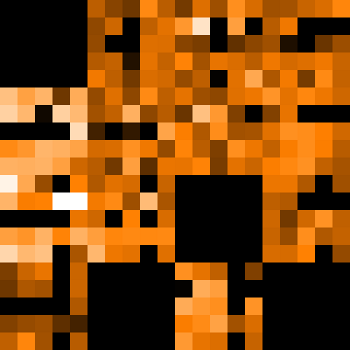
\includegraphics[width=5.2cm, height=5.2cm]{sc20_jiggle}
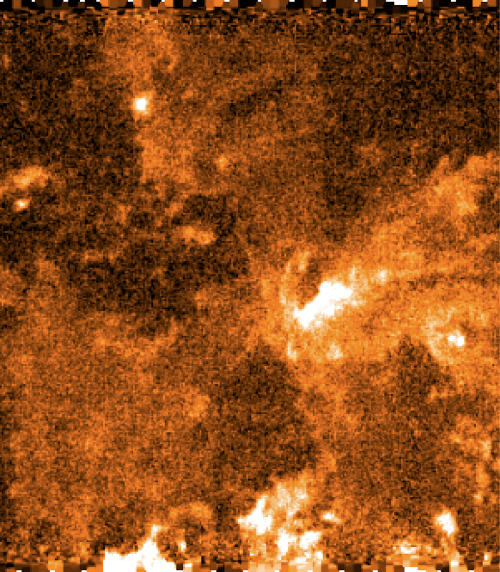
\includegraphics[width=5.2cm, height=5.2cm]{sc20_raster}
\caption[Stare, jiggle and raster observing modes]{\label{fig:harpmodes}
  (Left) Stare mode with HARP. (Right) Jiggle mapping with HARP.
  (Bottom) Raster mapping with HARP.}
\end{center}
\end{figure}


\section{\xlabel{obsmodes}Observing Modes}
\label{sec:obsmodes}

\subsection{On-source}

\begin{aligndesc}
\item[\textbf{Stare}]
A stare, or sample, observation is as simple as it sounds. When you
open reduced cubes of stare observations in \gaia\ you will see a map
consisting of one pixel for each receptor; one in the case of
$`$\=U$`$\=u, $`$\=Aweoweo and RxA and up to 16 with HARP. 
The left-hand panel of \cref{Figure}{fig:harpmodes}{} 
shows a stare observation (taken by HARP) opened in \gaia. You can also view the 
central spectrum using \linplot\ (see \cref{Appendix}{app:display}{Viewing 
your data with KAPPA}) or \splat.

\item[\textbf{Jiggle}]
A jiggle map is a common HARP observing mode. They are designed to
fill in the 30\arcsec spacing between the HARP receptors resulting in a
2\arcm$\times$2$\arcm$ map. This is achieved by 'jiggling' the secondary
mirror in a 4$\times$4 or 5$\times$5 pattern to give a HARP4 or HARP5
map respectively.  The HARP4 pattern has a 7.\uarcs5 pixels while the
HARP5 has 6\arcsec pixels, slightly under- and over-sampling compared
with Nyquist. The central panel of \cref{Figure}{fig:harpmodes}{} shows a
HARP5 jiggle pattern.

Each of these patterns can be pixel-centered, where the target
co-ordinates fall on one of the central four pixels, or map-centered where
the target co-ordinates lie at the centre of the map between the four
central pixels. See \cref{Figure}{fig:jiggle}{} for an illustration of the
different jiggle patterns. Although designed for HARP this mode can be
used with the single-element receivers.

\item[\textbf{Raster}]
Raster mapping, or scan mapping, is designed for mapping large areas
with maximum efficiency. The telescope continuously takes data while
scanning across the source. When HARP is used for raster mapping the
array is rotated 14.\udeg04 to the direction of the scan in order
to give a fully sampled map with 7.\uarcs3 pixels. This will result in
jagged edges to your reduced map which you may wish to trim. It is
common when using HARP to repeat the map scanning along the other axis
to give a `basket-weave' pair of maps. Each one of the pair will
appear as an individual observation.  The right-hand panel of Figure
\ref{fig:harpmodes} shows a HARP raster map.
\end{aligndesc}

\subsection{Reference}

\begin{aligndesc}
\item[\textbf{Position-switch}]

In position-switch (PSSW) mode, the whole telescope moves off source
and on to the reference position. This allows a large offset to the
reference position, useful in crowded environments such as the Galactic
Plane. The main disadvantage is that it takes a longer time resulting
in less-accurate sky subtraction or non-flat baselines.

\item[\textbf{Beam-switch}]
In beam-switch (BSW) mode, the secondary mirror chops onto the reference
position. This results in fast and accurate sky subtraction but it is
limited to targets which have a blank reference position within
180\arcsec (the maximum chop distance of the SMU).

\item[\textbf{Frequency-switch}]
In frequency-switch (FSW) mode the telescope does not move but the
centre of the spectral band is shifted, typically by 8 or 16\,Mhz,
to a line-free region of the spectrum. It is very efficient with no
off-source time and can be
useful when no emission-free reference position can be found.
\end{aligndesc}


\begin{figure}[b!]
\begin{center}
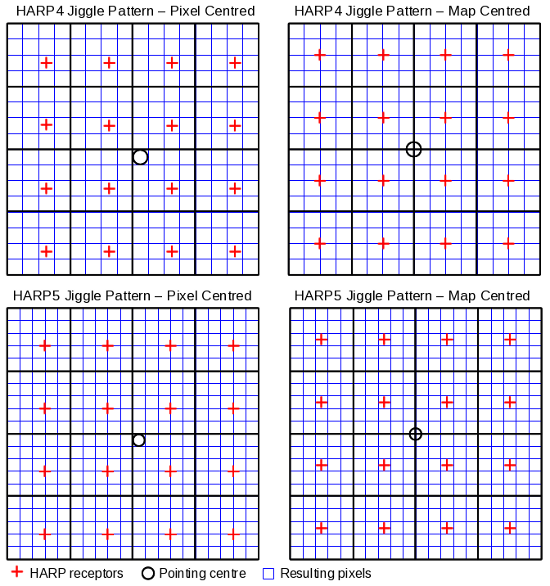
\includegraphics[width=0.8\linewidth]{sc20_jiggles}
\caption[HARP4 and HARP5 jiggle patterns]{\label{fig:jiggle}
  Top row: HARP4 jiggle patterns produce a map of 16$\times$16 pixels
  each of 7.\uarcs5. Bottom row: HARP5 jiggle patterns produce a map of
  20$\times$20 pixels each of 6\arcsec. }
\end{center}
\end{figure}

\subsection{Hybrid}
\label{sec:hybrid}

Subsystems are normally arranged to cover different spectral lines and
would be processed independently.  However, there is also a mode in
which the subsystems overlap in frequency, called \textbf{hybrid}.
Such data are combined to yield a broader spectral coverage, say where
there multiple lines in proximity.  The number of subsystems is a
power of two up to a maximum of four.

\clearpage
\chapter{\xlabel{data_files}Raw ACSIS Data}
\label{sec:raw}

\section{\xlabel{format}Data Format}
Raw ACSIS data follow this naming convention:

aUTDATE\_OBSNUMBER\_SUBSYSTEM\_SUBSCAN

For example, \file{a20131115\_00055\_03\_0001.sdf}. The first `a' represents
ACSIS. The UT date and observation number (OBSNUM) serve as an
identifier for any given night of observing. ACSIS observations may
include up to four frequency settings given by the different
subsystems (00-03), while long observations may require multiple
subscans to avoid a file size $>$512\,GB.

Within each data file each receptor is named. The naming system is 
zero-based. For HARP the receptor are labelled: H00, H01, H03... H015.
For the N\=amakanui inserts the names follow:

Instrument_Insert_Polarisation_Sideband

For example $`$\=U$`$\=u receptors are: NU0L, NU0U, NU1L, NU1U, 
with U denoting the insert. For $`$\=Aweoweo, W denotes the insert: 
e.g. NW0L, NW0U, NW1L, NW1U and for  Ala$`$ihi, A denotes the insert. 

\section{\xlabel{visualise}Visualising raw data}
\label{sec:exam}

Use the \starlink\ application \gaia\ to visualise your raw data. The
is initiated by:

\begin{terminalv}
% gaia rawfile
\end{terminalv}

Loading a file in \textsc{Gaia} produces two to three windows (see
\cref{Figure}{fig:rawgaia}{the first figure below} and
\cref{Figure}{fig:ndfgaia})). The main window
shows a map of the HARP receptors (along the $x$-axis; note the 16
pixels) for a given sample of the observation (time on the $y$-axis).
You can track the performance of an individual receptor by following a
column from bottom to top to check its consistency. In
\cref{Figure}{fig:rawgaia}{the first figure below} H03 is dead for the
whole observation. The spectrum for a receptor at one of the time
slices can be seen by clicking on the pixel. This will bring up
another window---the \guiwindow{Spectral plot} (see
\cref{Figure}{fig:gaia2}{the second figure below}). This spectrum will
be replaced when you click on a different pixel.

You can change the way the data is displayed in the \guiwindow{Display
image sections of a cube} window by changing the \guithing{Axis}.
Selecting Axis number two will display spectra against time while Axis
number three gives spectra against receptors. You can scroll through
your data by moving the \guithing{Index of plane} slider.

\begin{figure}[h!]
\begin{center}
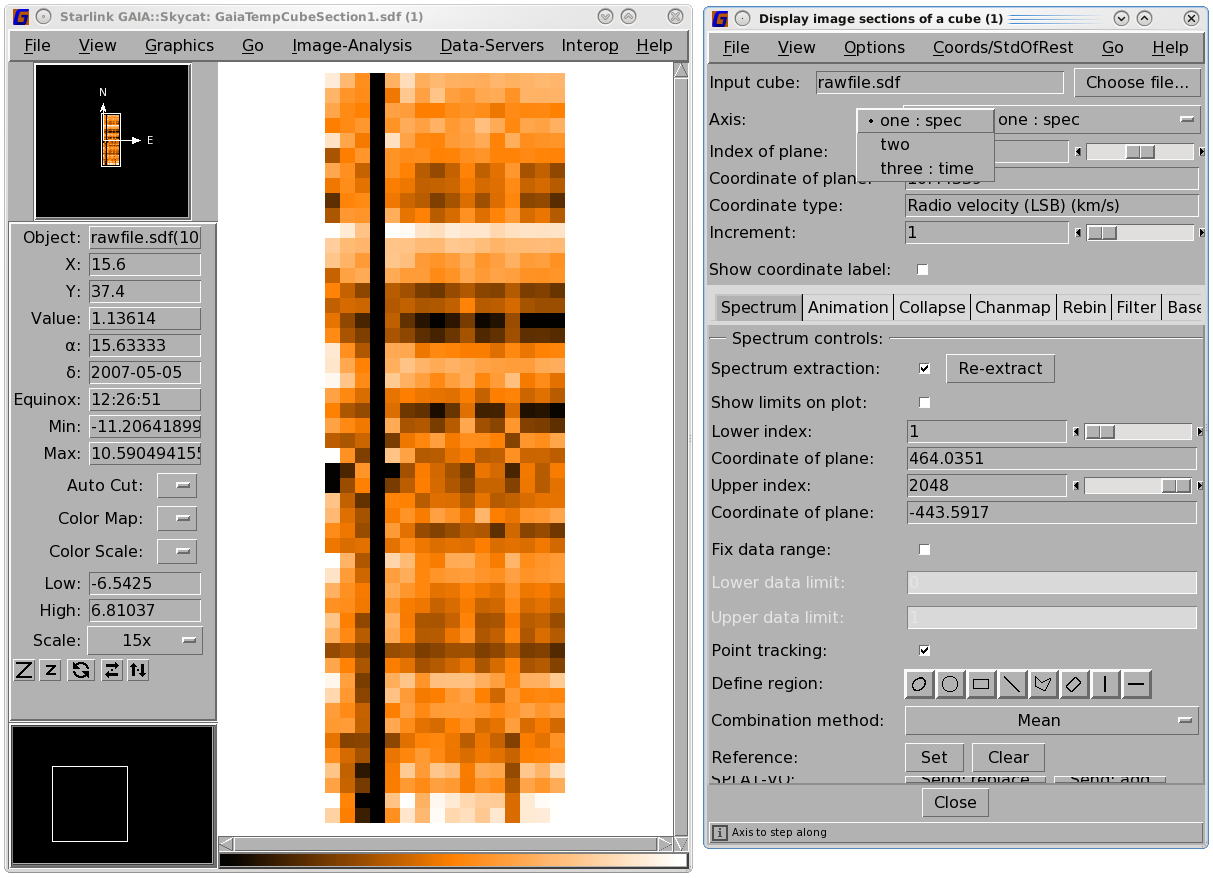
\includegraphics[width=0.9\linewidth]{sc20_gaia1}
\typeout{sc20_gaia1 inserted on page \arabic{page}}
\caption[\gaia\ main window.]{\label{fig:rawgaia}
  Initial \textsc{Gaia} windows displayed upon loading a raw
  data file. The main window on the left shows a map of receptors at
  given time-samples during the observation. You may have to zoom in
  multiple times by clicking the large \guithing{Z} button on the side
  panel. On the right, the \guiwindow{Display image sections of a cube}
  window enables you to navigate the time axis.}
\end{center}
\end{figure}


\begin{figure}[h!]
\begin{center}
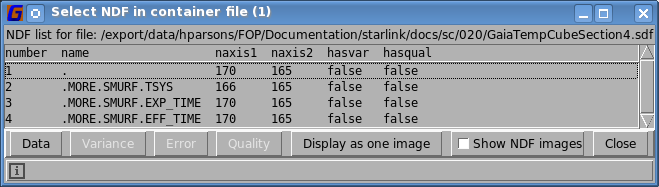
\includegraphics[width=0.7\linewidth]{sc20_gaia3}
\typeout{sc20_gaia3 inserted on page \arabic{page}}
\caption[\gaia\ select NDF in container file]{\label{fig:ndfgaia}
  Select the NDF from the container file.  This window is displayed upon
  loading a new file in \textsc{Gaia}.  In this example, you can choose
  from NDFs holding the data, the system temperatures, the effective
  times, and the exposure times.}
\end{center}
\end{figure}


\begin{figure}[h!]
\begin{center}
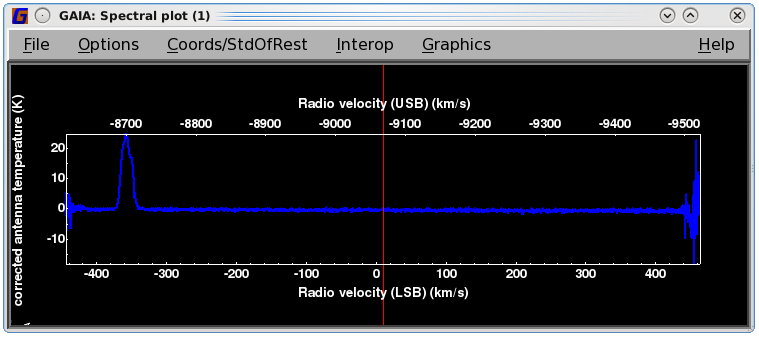
\includegraphics[width=0.7\linewidth]{sc20_gaia2}
\typeout{sc20_gaia2 inserted on page \arabic{page}}
\caption[Spectral plot window with \gaia.]{\label{fig:gaia2}
  The \guiwindow{Spectral plot} window displaying its time-varying
  signal, appears automatically once a pixel is clicked in the main window.
  The vertical red line indicates the time slice that is currently selected
  in the \guiwindow{Display image sections of a cube} window. This can be
  dragged across the spectrum to scroll through the spectra. Examine exposure
  time map etc. in ancillary arrays.}
\end{center}
\end{figure}



A second way to scroll through your spectrum is to click and drag the
vertical red bar on the \guiwindow{Spectral plot} window. As you do so
array shown in the main window will automatically update.

You will likely want to change the auto cut of the colour scale, the
colour scheme and the zoom factor---all of which are controlled by
buttons on the sidebar in the main window.

See the \xref{\textsc{Gaia} manual}{sun214}{} for full
details.

\section{\xlabel{maskbad}Identifying and Masking Bad Data}
\label{sec:badrecs}

You can mask bad receptors in the time-series data with the \Kappa\
command \chpix. In the HARP example below all data for Receptors 7 and 8
(on the second axis) are turned off by setting them to BAD. Note the
commas in the \param{SECTION} parameter which specify which axis is
being referred to; here the first (spectra) and third (time) axes are
unchanged so no range is defined. You will have to repeat the command
for non-contiguous receptor numbers.

\begin{terminalv}
% chpix in=raw out=raw_masked section="',7:8,'" newval=bad
\end{terminalv}
You can also mask a subset of the time stream for a particular
receptor. The example below masks out time Steps 18 to 33 for HARP receptor
H01. See \cref{Figure}{fig:maskreceptor}{} for instructions on how to
identify the affected time range.
\begin{terminalv}
% chpix in=raw out=raw_masked section="',1:1,18:33'" newval=bad
\end{terminalv}
Note that the numbering for the 16 HARP receptors here is 1--16; this is in
contrast to 0--15 that you will encounter with the pipeline.

For jiggle maps, where the receptors do not cover multiple sky
positions, bad receptors can be identified in the reduced cubes. For
raster maps, however, bad receptors are most easily identified in the
time-series data. Once you have opened your raw cube in \gaia\ it is
useful to select the second axis (receptor) which gives spectral
dispersion along the $x$-axis and time along the $y$-axis. You can use
the cube control panel to step through each receptor looking for bad
spectra (see \cref{Figures}{fig:maskreceptor}{} and
\ref{fig:maskreceptor2}).

\begin{figure}[h!]
\begin{center}
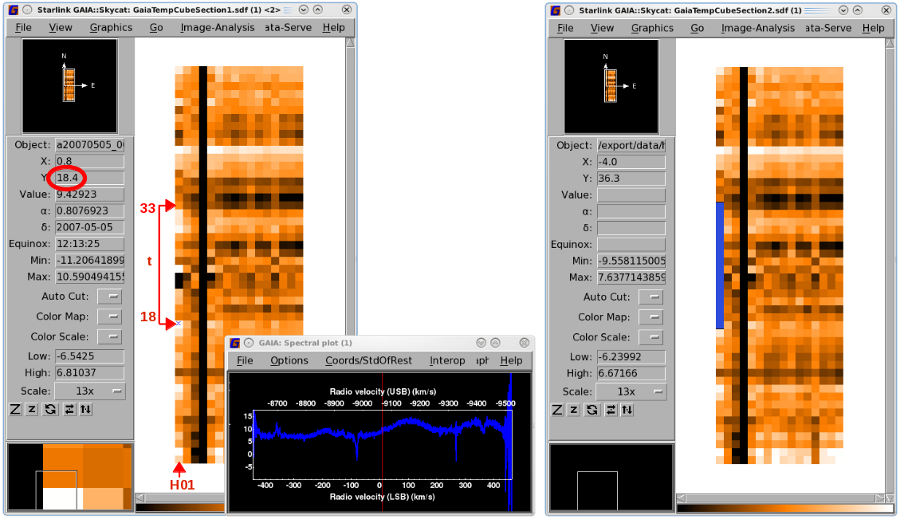
\includegraphics[width=1\linewidth]{sc20_maskreceptor}
\typeout{sc20_maskreceptor inserted on page \arabic{page}}
\caption[Identifying bad receptors in the raw data.]{\label{fig:maskreceptor}
  The left-hand \gaia\ window shows raw HARP data before masking.
  Clicking on a pixel will show the spectra. The spectrum shown is from
  receptor H01 at Step 18 (see circled $Y$ value). To mask this receptor
  in time from Step 18 to 33---at which point the bad baselines
  disappear---use \chpix. The right-hand \gaia\ window shows the raw
  data after masking where the time range in question is now blank.}
\end{center}
\end{figure}

\begin{figure}[h!]
\begin{center}
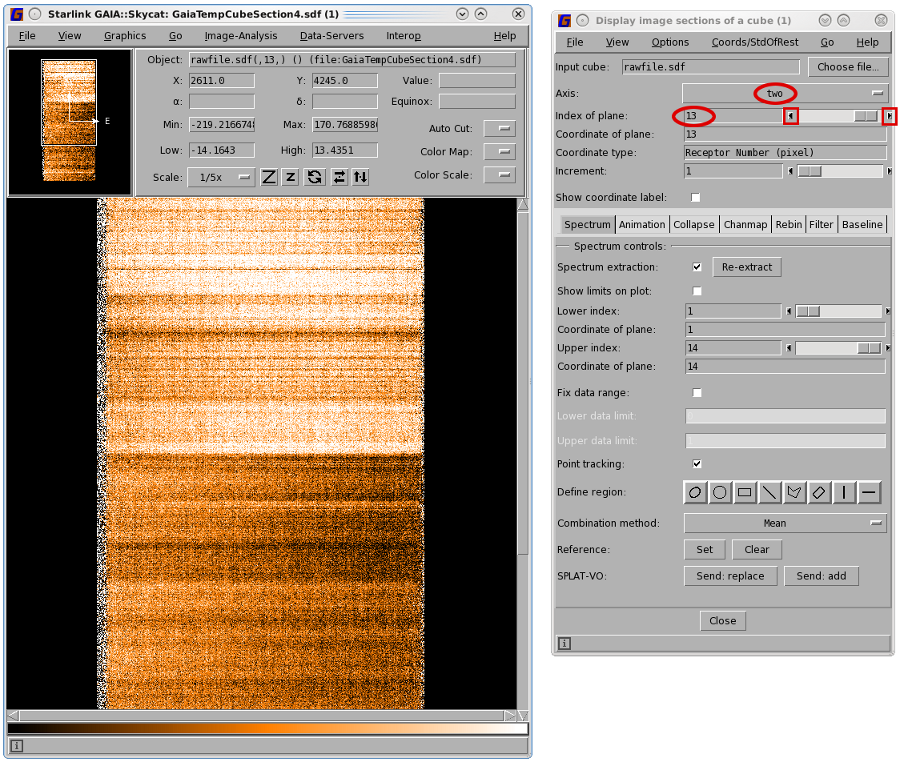
\includegraphics[width=0.9\linewidth]{sc20_badreceptor2}
\typeout{sc20_badreceptor2 inserted on page \arabic{page}}
\caption[Identifying bad receptors in the raw data: second method.]{\label{fig:maskreceptor2}
  In this example, the second axis (receptor number) has been
  selected. Use the arrows outlined in red on the \guithing{Index of
  plane} bar to scroll through the receptors. Here you can see
  Receptor 13 (see circled \guithing{Index of plane} value) which
  goes noisy two-thirds the way through the observation.}
\end{center}
\end{figure}


\newpage
\chapter{\xlabel{pipeline}The ACSIS Pipeline}
\label{sec:pipe}

The \ORACDR\ pipeline \cite{oracdr} is a generic automated data
reduction pipeline that can process your raw JCMT data and return
advanced data products: baselined single observation cubes, mosaicked
and co-added cubes, moments map and clump catalogues.
\cite{heterodyne_pipeline}

It has advanced algorithms for the common routines such as baseline
subtraction. The data processing is performed using standard \Kappa,
\smurf, and \cupid\ applications, the main ones of which are
described in later chapters.

\section{\xlabel{recipes}Recipes and primitives}
\label{sec:recipes}

Reduction recipes in \ORACDR\ consist of a series of stand-alone
processes, known as primitives. These primitives are linked together
to form data reduction recipes. Each primitive can be fed different
input data depending on the nature of the recipe in question and may
sometimes be omitted altogether.

There are four main science recipes available, each tailored to different
type of observation:
\begin{itemize}[noitemsep,,nolistsep]
\item \narrowline\\
\item \broadline\\
\item \gradient\\
\item \lineforest
\end{itemize}

A summary of these recipes is given below.

\begin{table}[h!]
\begin{tabular}{p{2.9cm}|p{7.3cm}|p{4.5cm}}
\hline
\textbf{RECIPE} & \textbf{DESCRIPTION OF EMISSION} & \textbf{BASELINE METHOD} \\
\hline
NARROWLINE & One or more narrow lines are expected across the band.
Select this recipe if the expected lines are less than about
8~\kms\ wide.& Smoothing: \newline spatial = 5$\times$5 pixels
\newline frequency = 10 channels\\
\hline
BROADLINE &This recipe is designed for wide lines that extend over a
large fraction of the band. The line is typically too weak to see in a
single observation so a pre-determined baseline window and linear
baselines are used.  &Uses the outer 10\% of each end of the spectra
to fit a single-order polynomial.  \\
\hline
GRADIENT &Typically one moderately wide line is expected, for which
the center velocity varies significantly across the field. The
baseline window changes across the field. Nearby galaxies often fall
in this category. The expected lines should be wider than about
8~\kms\ and probably not wider than 20\% of the available bandwidth &
Smoothing: \newline spatial = 3$\times$3 pixels \newline frequency =
25 channels\\
\hline
LINEFOREST & A forest of lines is expected across the band. Bright,
nearby star-formation sources may fall in this category.  This recipe
also creates a separate moments map for each line (as defined by the
parameter \param{PER\_LINE}).& Smoothing: \newline spatial = none
\newline frequency = 10 channels \\
\hline
\end{tabular}
\end{table}

There are also variants of the recipes with the following suffixes.

\begin{tabular}{p{2cm}p{10cm}}
\_POL & polarimetry \\
\_QL & Quick Look which merely runs \makecube\ to turn the raw time-series
spectra into a spectral cube for display during data acquisition. \\
\_SUMMIT & A limited reduction to keep pace with data acquisition at the
JCMT.  It excludes any bad spectra rejection, quality assurance, or
iterative baseline determination. \\
\end{tabular}

\newpage
\section{\xlabel{recipe_process}The workflow}
You can follow this commentary via the flow chart in
\cref{Figure}{fig:pipeline}{below}.

Two notations are used in the following list:\\
\textbullet\ \textbf{a\_cube} to mean the regridded cube of a single
observation. \\
\textbullet\ \textbf{g\_cube} to mean the group cube which is a co-add
of all the \textbf{a\_cube} files.

Note that the pipeline will co-add data into a group file whenever it
encounters observations with identical LO frequencies, base positions
and bandwidths.  You can also force a set of observations, such as
ones of the same object taken on different nights, to be regarded as
a single group to be combined via the \texttt{oracdr -onegroup}
command-line option.

\begin{enumerate}[label=(\textbf{\arabic*})]

\item The raw data is copied to the local directory. Typically,
subsystems are treated as individual and separate observations by
\ORACDR\ except for hybrid-mode observations.

\item Because data acquisition is asynchronous, time slices are not
necessarily written in sequential order. The next step sort the
time-series data into time order. This makes it easier to search for
intermittent bad data.

\item The noisy ends of the spectral band dwarf most
astronomical signal, and hence are removed as follows.
The spectra are collapsed along the receptor using the `sigma'
estimator to form a single spectrum. A constant value background is
then fit to the resulting spectrum. The fitting regions are used to
determine where the spectrum gets noisier (i.e. higher RMS values in
the RMS spectrum). These high-noise regions are then trimmed from the
ends in the frequency axis.   There is also an alternative to trim
specified percentages through the \param{TRIM\_} recipe parameters
(see \cref{Table}{tab:trim_params}{}).

\item The DC-level offset between corresponding sub-band observations
is determined using the median of all the spectra.  The DC offset is
then subtracted from the sub-band spectra, and the resulting sub-band
spectra are mosaicked together to form single time-series cube.

\item Regions or individual spectra containing high- and low-frequency
interference from local sources are identified and flagged.  Bad
detectors are identified by comparing the deviation from linearity of
each detector's baseline.

\item Strong spikes ($\pm$150) are replaced by bad values.

\item Quality assurance checks are run on the raw cubes. See Appendix
\ref{app:qa} for a description of the checks performed. Any
time-slices failing any of these checks gets flagged as bad and
are not included in the group co-add that follows.

\item Once all the raw observations have undergone the initial
processing, the individual time-series files are combined to form a
\textbf{g\_cube}.

\item \label{step:loop}
The \textbf{g\_cube} is smoothed by an amount specified by the
particular science recipe being used. See
\cref{Section}{sec:recipes}{Recipes and primitives}
for details on the different recipes.

\item \mfittrend\ is run to find the baseline regions on the smoothed
\textbf{g\_cube}. The ranges are determined automatically by setting
\param{auto=true}. A baseline mask is written out.

\item The baseline mask is then applied to the unsmoothed
\textbf{g\_cube} and \mfittrend\ is re-run. This time however, the
emission regions have been masked out, so all remaining data are
included in the fit by setting \param{auto=false}. The resulting
baseline is subtracted.

\item Moments maps and noise maps are made from the
baseline-subtracted \textbf{g\_cube}.

\item If another iteration is required, continue to
\cref{Step}{step:iterate}{}. If not, the processing is complete.

\item \label{step:iterate}
The baseline mask is converted back to the time series with
\unmakecube. There it is applied to the time-series data for each
observation.

\item A baseline is fit to the masked time-series data using
\mfittrend\ and the result is subtracted from the unmasked time-series
data.  This can be a higher-order polynomial (up to
15$^{\textnormal{th}}$ order), although a linear fit is often used.

\item A flat field, i.e. the relative responsivities of the detectors,
is optionally created and applied.  It involes making cubes for each
each receptor combining all observations on a given date to improve
the accuracy.  There is a choice of analysis methods, but an
iterative approach of thresholding---to exclude the noisy baseline
that would dilute the comparisons---worked best on most suitable
observations.  Those with low signal-to-noise or signal only
originating in a small percentage of the area mapped are not amenable
to determining the receptor-to-receptor responses.  (See
\cref{Table}{tab:flat_params}{}).


\item An \textbf{a\_cube} is made from the baseline subtracted data
for each observation.

\item The individual baseline-subtracted time series are combined
to make a new \textbf{g\_cube}.

\item Return to \cref{Step}{step:loop}{}.
\end{enumerate}

%\setlength{\intextsep}{10.0pt plus 1.0pt minus 2.0pt}
\begin{figure}[h!]
\begin{center}
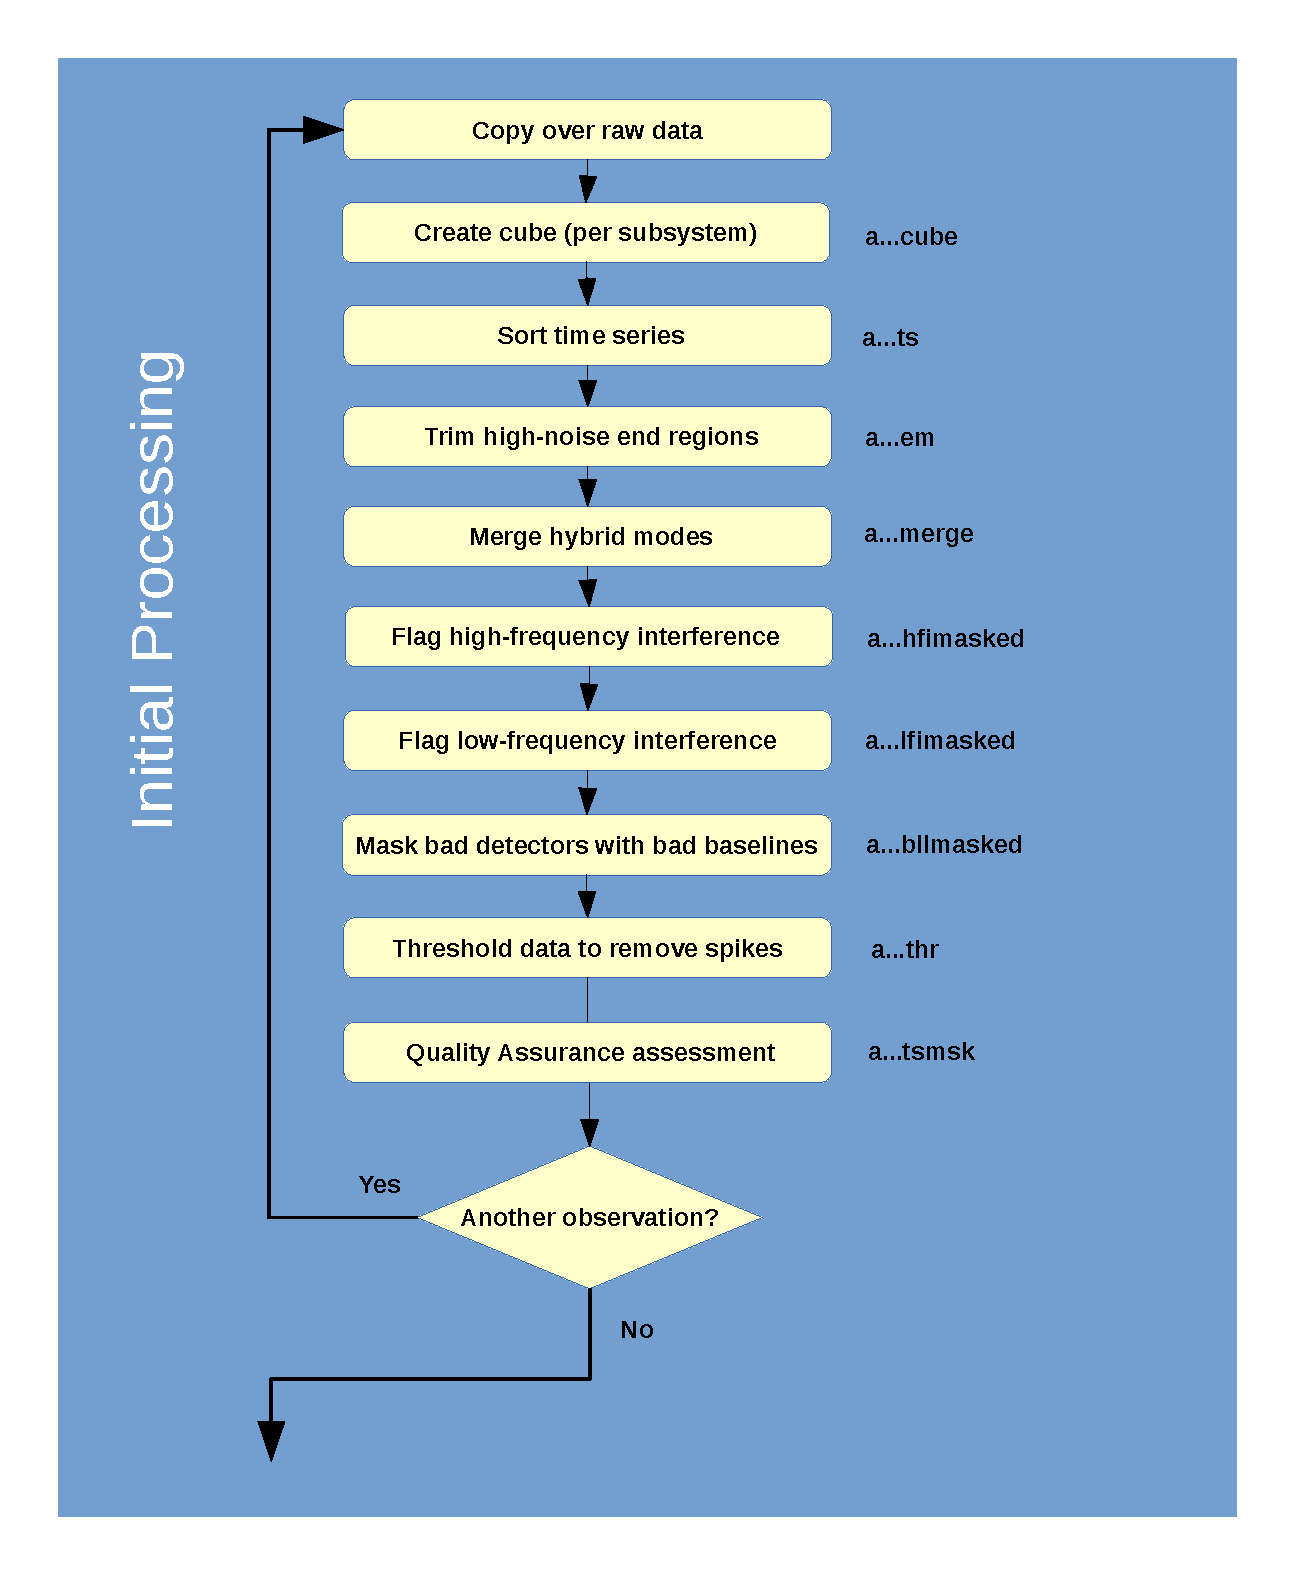
\includegraphics[width=0.81\linewidth]{sc20_workflow_initial}
\end{center}
\end{figure}

\begin{figure}[h!]
\begin{center}
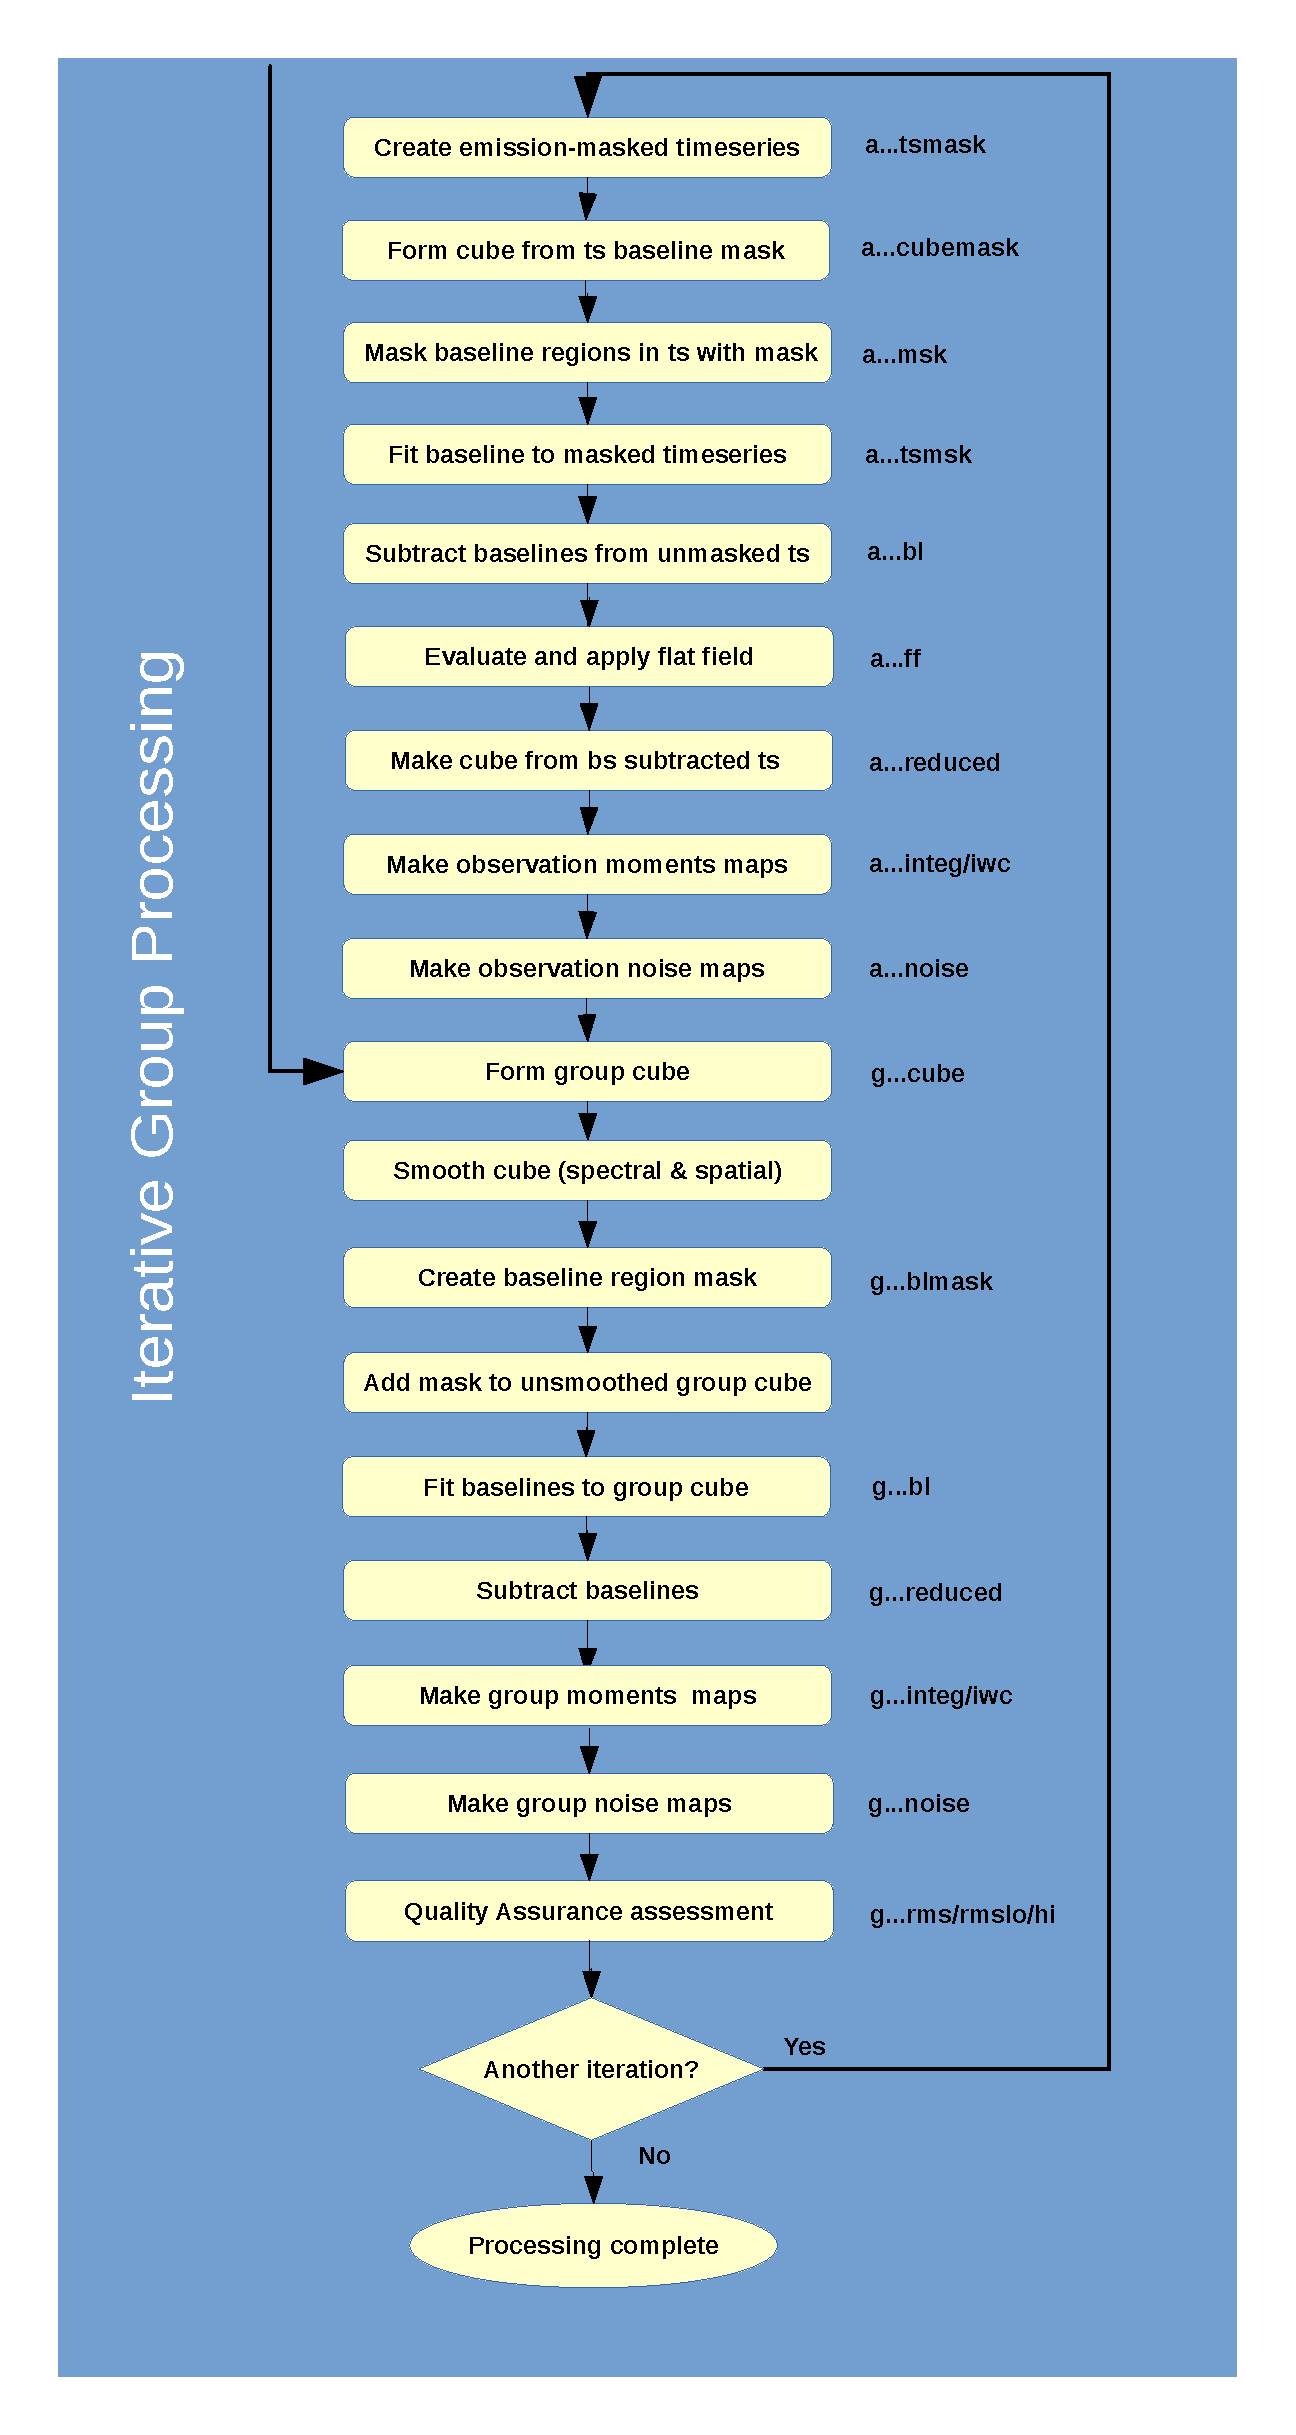
\includegraphics[width=0.81\linewidth]{sc20_workflow_group}
\end{center}
\end{figure}
\clearpage

\begin{figure}[h!]
\begin{center}
\caption[Flow chart of the \ORACDR\ ACSIS pipeline process.]{\label{fig:pipeline}
  Flow chart of the processes employed by the \ORACDR\ ACSIS pipeline,
  specifically the \narrowline\ and \gradient\ recipes. A few minor processing
  steps are omitted to avoid the diagram being too long. Other recipes may have
  additional steps or omit steps as appropriate. Because of space
  constraints baseline is sometimes abbreviated to `bs' and time series
  to `ts' in the step descriptions.  The prefix and suffix of the file
  created at each stage is shown to the right of the process box.
  Note that suffix `a' refers to an individual observation, while `g'
  refers to a group (or co-added) file.}
\end{center}
\end{figure}
\setlength{\textfloatsep}{20pt plus 1.0pt minus 2.0pt}

\clearpage
\chapter{\xlabel{running_pl}Running the pipeline}
\label{sec:runpipe}

\section{Checking and changing the science recipe}
\label{sec:changerecipe}
You can find out which recipe is set in the data header via the
\param{RECIPE} keyword in the FITS header of any of your raw files.
You can use either of the options below:
\begin{terminalv}
% fitsval a20130609_00059_01_0001 RECIPE
% fitslist a20130609_00059_01_0001 | grep RECIPE
\end{terminalv}

You can override the recipe set in the FITS header by listing any different
one on the command line when starting \ORACDR. For example:
\begin{terminalv}
% oracdr -file mylist -loop file -log x REDUCE_SCIENCE_GRADIENT
\end{terminalv}

\section{Setting recipe parameters (optional)}
\label{sec:recpars}

You can tailor the recipe parameters by supplying a \file{.ini} file
(called \file{myparams.ini} in the following example). This file contains the
recipe name (which must match the one assigned to your data, whether
from the header or any different one specified on the command line)
followed by the options you wish to specify in the following format:

\vspace{0.2cm}
\begin{terminalv}
[REDUCE_SCIENCE_NARROWLINE]
MOMENTS_LOWER_VELOCITY = -30.0
MOMENTS_UPPER_VELOCITY = 155.0
PIXEL_SCALE = 6.0
SPREAD_METHOD = gauss
SPREAD_WIDTH = 9
SPREAD_FWHM_OR_ZERO = 6
REBIN = 0.635,2.0
\end{terminalv}

Notice the two values given for the \param{REBIN} option. This means
that two maps will be produced, one at each of the specified velocity
resolutions. See \cref{Appendix}{app:params}{Classified Recipe
Parameters} for a full list of recipe
parameters.

The \file{.ini} file can contain an arbitrary number of \param{[]}
constructs for different recipes, qualified by object name or
\ORACDR\ internal headers.

While the use of recipe parameters is optional, once you have some
experience with the pipeline you are encouraged to tailor the recipe
parameters for your reductions to get the best out of the recipe and
your data.

\subsection{Setting recipe parameters by object name}
\label{sec:recpars_object}

You can further select the recipe parameters by object name, as given
by the OBJECT FITS header converted to uppercase with spaces removed.
Here are some examples.

\vspace{0.2cm}
\begin{terminalv}
[REDUCE_SCIENCE_BROADLINE:NGC253]
REBIN = 10.0,20.0,30.0
PIXEL_SCALE = 15.0
\end{terminalv}

This would apply the two recipe parameters to the NGC~253 target
when processed by REDUCE\_SCIENCE\_BROADLINE, while

\vspace{0.2cm}
\begin{terminalv}
[REDUCE_SCIENCE_BROADLINE:ARP*]
REBIN = 10.0,20.0,30.0
PIXEL_SCALE = 15.0
\end{terminalv}

would apply the same parameter values for any beginning with the Arp
designation.

\subsection{Setting recipe parameters by ORAC-DR internal header}
\label{sec:recpars_orac}

The pipeline translates a selection of metadata from the FITS headers
into \oracdr\ internal headers.  You can choose different sets of recipe
parameters from the internal headers.  The available headers can be
inspected with \task{translatehdr} supplied with one of your raw data
files.

\vspace{0.2cm}
\begin{terminalv}
% $STARLINK_DIR/Perl/bin/translatehdr a20151213_00067_01_0001.sdf
\end{terminalv}

Here is an example of how to select by internal header.

\vspace{0.2cm}
\begin{terminalv}
[REDUCE_SCIENCE_NARROWLINE#SAMPLE_MODE=GRID]
LV_IMAGE = 1
LV_AXIS = skylon
\end{terminalv}

would apply these parameters only to data whose sample mode was grid.

You can select by an arbitrary number of internal headers to
narrow the selection.  The internal headers must follow any object name
as in the following example.

\vspace{0.2cm}
\begin{terminalv}
[REDUCE_SCIENCE_NARROWLINE:HH21#SPECIES=C-18-O#BANDWIDTH_MODE=250MHzx4096]
FINAL_LOWER_VELOCITY = -100
FINAL_UPPER_VELOCITY = 100
MOMENTS_LOWER_VELOCITY = 1.2
MOMENTS_UPPER_VELOCITY = 6
FLATFIELD = 0
\end{terminalv}

\param{SPECIES} defines the molecule.  The rationale for this might be
disable estimation of the flat field because the signal is much weaker
for the molecule C$^{18}$O.  Other common values are \texttt{CO} for
$^{12}$CO and \texttt{13-CO} for $^{13}$CO.  There is also a
\param{TRANSITION} header to select by the transition.

The velocity limits for the moments might be set narrower than for
other molecules.  You might want to set a different velocity range in
the final spectral cubes (set by the \param{FINAL\_LOWER\_VELOCITY} and
\param{FINAL\_UPPER\_VELOCITY} parameters) depending on the spectral
resolution given by \param{BANDWIDTH\_MODE} (see
\cref{Figure}{fig:backend}{} for a list).


\section{Setting quality-assurance parameters (optional)}
\label{sec:qa}

There is a set of quality-assurance (QA) parameters that are applied
by default when you run the pipeline. These are found in the text file
\file{\$ORAC\_DATA\_CAL/qa.ini}.

You can set your own QA parameters by creating a local \textit{.ini}
file (called \file{myqa.ini} in the following examples). You can then call
this local QA file via \param{-calib qaparams=myqa.ini} when starting
the pipeline.

The example below illustrates the format of this QA file and
highlights some of the main parameters you may consider tweaking.

\vspace{0.2cm}
\begin{terminalv}
[default]
BADPIX_MAP=0.1
GOODRECEP=8
TSYSBAD=550
FLAGTSYSBAD=0.5
TSYSMAX=550
TSYSVAR=1.0
RMSVAR_RCP=0.5
\end{terminalv}
The text in the square brackets describes the data to which the QA
parameters should be applied. This is followed by the QA parameters
and their values.

The parameters listed under the [default] header will get picked up
for \textit{all} observations unless overridden by other header
descriptions. Extra header may describe a frequency range (e.g.
\texttt{[default 200:300]}), a particular molecule and transition
(e.g. \texttt{[default CO32]}), an instrument (e.g. \texttt{[RXA]}),
or a legacy survey (e.g. \texttt{[GBS]}). You can also include
combinations (e.g. \texttt{[GBS\_13CO32]}). Note that for any data
taken by RxA or RxW, \param{GOODRECEP} must be set to 1.

The example file below sets up a different set of parameters for two
transitions of CO. Any QA parameters not explicitly set will revert to
those specified in the default \file{qa.ini} file.

\vspace{0.2cm}
\begin{terminalv}
[C18O32]
RES_CHAN=10
VELRES=1.0
TSYSBAD=650

[CO21]
RES_CHAN=10
VELRES=0.5
TSYSBAD=550
GOODRECEP=1
\end{terminalv}

See \cref{Appendix}{app:qa}{Quality Assurance Parameters} for a
description of all available QA parameters.


\section{Specifying bad receptors (recommended)}
\label{sec:badrec}

If certain receptors are known to be bad for the full length of an
observations (e.g. dead receptors), processing time can be reduced by
not having the pipeline attempt to reduce that data. The ability to 
masking bad receptors also provides an additional tool for those wishing 
to examine data in more detail (e.g. when looking at data from an 
instrument that has yet to be fully commissioned).

Information regarding bad receptors is stored in a master text file
called \file{index.bad\_receptors}, located in your
\file{ORAC\_DATA\_CAL} directory. This file lists dates and the
corresponding receptors which are not operational. By default, when
the pipeline runs it searches this file and discards the appropriate
receptors. However, this master list is grossly incomplete so you
should select another method for specifying bad receptors.

We recommend using the \param{index} option, called via \param{-calib
bad\_receptors=index} when starting the pipeline. This creates an
index file called \file{index.bad\_receptors\_qa} in your
\file{ORAC\_DATA\_OUT} directory, where any bad receptors identified
during your reductions are indexed. This file is appended each time
you run the pipeline and in this way you build up your own independent
list.

If an index file exists, then, by default, the pipeline will look for
bad-receptor information in both
\file{\$ORAC\_DATA\_CAL/index.bad\_receptors} and
\file{\$ORAC\_DATA\_OUT/index.bad\_receptors\_qa}.

\begin{table}[h!]
\begin{tabular}{p{3cm}|p{12cm}}

\textbf{bad\_receptors} & \textbf{Description} \\
\hline
masterorindex & Use both the master \file{index.bad\_receptors} and pipeline-generated
                \file{index.bad\_receptors\_qa} files [Default].\\
master        & Use the master \file{index.bad\_receptors} file in \file{\$ORAC\_DATA\_CAL}. \\
index         & Use the \file{index.bad\_receptors\_qa} index file in
                \file{\$ORAC\_DATA\_OUT} as generated by the pipeline. \\
file          & Reads a file called \file{bad\_receptors.lis}, which
                should contain a space-separated list of receptor names in the
                first line. This file must be located in \file{\$ORAC\_DATA\_OUT}
                and invoked by \param{-calib bad\_receptors=file}.\\
list          & A colon-separated list of receptor names can be supplied, such as
                \param{-calib bad\_receptors=H01:H06}, or \param{-calib 
                bad\_receptors=NU1L,NU1U}. You can append any of the other
                options to the end of your list, such as \param{-calib bad\_receptors=H14:index}\\
\hline
\end{tabular}
\caption[Pipeline options for the \param{-calib bad\_receptors} flag.]{\label{tab:index-options}\small
  The options available for the \param{-calib bad\_receptors} flag when running
  the pipeline.}
\end{table}

When reduced by \makecube\ - either by hand or through the pipeline - it
is possible to find out which receptors are present in the data by inspecting the
reduced data file's FITS header. This can be done using \fitslist\ or fitsval and 
looking at the RECPUSED parameter.

\begin{terminalv}
% fitsval a20200808_00084_01_reduced001.sdf RECPUSED
NU0L NU1L
\end{terminalv}

\section{\xlabel{starting_pl}Starting the pipeline}
\label{sec:runpl}

\begin{enumerate}[label=(\textbf{\arabic*})]

\item Initialise the pipeline software.  This may be as simple as

\begin{terminalv}
% oracdr_acsis
\end{terminalv}

\item Define environment variables to ensure the data is read from,
and written to, the right place. Many are set automatically when the
pipeline is initialised but others must be set manually. Details of
the optional variables are given in \acsispipelinesun\ but you should
specify where to find the raw data and where to write any files that
are created.
\begin{terminalv}
% setenv ORAC_DATA_IN <path to raw data>
% setenv ORAC_DATA_OUT <where you want reduced data to go>
\end{terminalv}

These extra definitions can be avoided if you initialise with the
following command.

\begin{terminalv}
% oracdr_acsis -cwd
\end{terminalv}

The \param{cwd} option requests that the current working directory is
used for all input and output, which is most likely what you require.

If you are supplying a text file listing the raw data
\file{\$ORAC\_DATA\_IN} should be the location of this file. If
supplying an external configuration file it should also be in this
location.

If you wish to keep the intermediate files produced by the pipeline
you should also set \param{ORAC\_KEEP}.
\begin{terminalv}
% setenv ORAC_KEEP 1
\end{terminalv}
However, this still excludes temporary files made during a recipe step,
whose names have the \file{oractemp} prefix.  To retain these set
\begin{terminalv}
% setenv ORAC_KEEP temp
\end{terminalv}

Retention of temporary and intermediate will require plenty of storage,
but it can be invaluable during debugging.

\item Now you are ready to run the pipeline. In this example, the
recipe name on the end ensures that all data being processed using
\narrowline.

\begin{terminalv}
% oracdr -files list.txt -loop file -batch -log xf -calib qaparams=myqa.ini \
  bad_receptors=index -recpars mypar.ini -nodisplay REDUCE_SCIENCE_NARROWLINE
\end{terminalv}
\end{enumerate}

Below is a list of commonly used command line options when running the
\ORACDR\ pipeline from outside the EAO. For a full list of all possible
options and their descriptions see \oracdrsun.
\begin{table}[h!]
\begin{tabular}{p{2.5cm}|p{12.5cm}}

\textbf{Flag} & \textbf{Description} \\
\hline
\multicolumn{2}{l}{\textbf{Supplying data}} \\
\hline
%-from/-to         & Number of first/last observation \\
%-list             & Comma separated list of observation numbers \\
-file $<$mylist$>$ & Input data provided by a text file. Supply the
                     file name (relative to current directory, or the full
                     path) of an ASCII text file containing a list of all
                     observation files to be reduced, one file per line. \\
%-ut               & UT date of observations (defaults to current \emph{yyyymmdd}). \\
\hline
\multicolumn{2}{l}{\textbf{Looping}} \\
\hline
%-loop list & Default when using the -list option. The pipeline will stop once
              the observations in the list have been reduced. \\
-loop file  & Loop over all the lines in the file supplied by the \param{-file}
              option. \\
\hline
\multicolumn{2}{l}{\textbf{Group processing}} \\
\hline
\param{-batch}    & Delays group processing until the individual files have been reduced.  \\
%\param{-skip}    & Allow the data detection loop to skip missing observations.  \\
\param{-onegroup} & Forces all the observations into the same group. Useful if
                    building up a map from rasters with different target co-ordinates
                    or from different dates.  \\
\hline
\multicolumn{2}{l}{\textbf{Supplying parameter files}} \\
\hline
\param{-calib}    & Under the calibration flag you can specify QA parameters by including
                    \param{qaparams=<myqa.ini>} and bad receptors via
                    \param{bad\_receptors=index}.  If you do not set the
                    \texttt{qaparams} option but have a file called \file{qa.ini}
                    in your output directory, the QA settings will come from this file.\\
-recpars & Allows you to provide recipe parameters as a \file{.ini} file.  \\
\hline
\multicolumn{2}{l}{\textbf{Logs/Display}} \\
\hline
\param{-nodisplay} & Shorten processing times by turning off all graphical output. \\
\param{-log sxfh}  & Send the log to a screen (\param{s}), an xwindow (\param{x}), file
                     (\param{f}) or html (\param{h}). The logfile
                     (\param{f}) has the name \file{.oracdr\_}$NNNN$\file{.log} where
                     $NNNN$ is the current process ID. Only include the options you want.
                     This defaults to \param{xf}.\\
\hline
\end{tabular}
\caption{\small \label{tab:pipe-options}
  The options available on the command line when running the \ORACDR\ pipeline from outside
  the EAO.}
\end{table}

\section{\xlabel{pl_output}Pipeline output}

The pipeline will produce a group file for each object being
processed. If the pipeline is given data from multiple nights, all
those data will be included in the group co-add using inverse variance
weighting.

Files created from individual observations are prefixed with
\file{a}, while group (co-added) maps are prefixed with \file{ga}.
\cref{Table}{tab:pipe-out}{the table below} describes the files
created. In addition PNG images are made of the reduced files at a
variety of resolutions.

\begin{tip}
TIP: Even if just a single observation is processed, a group file is
created so long as the observation passes the QA check.
\end{tip}

\subsection{Why have multiple reduced files been generated?}
\label{sec:multireduced}

You will find the pipeline splits large reduced cubes (e.g. from
raster maps) into smaller tiles of $<$512\,MB. This is to save on
computer memory. It does this from the central position outwards so
you may find some of the smaller edge tiles are strange, often narrow,
rectangles. These tiles can be pasted together with the \Kappa\
command \paste\ but beware of the final file size. For example,
\begin{terminalv}
% paste ga20140601_15_1_reduced\*.sdf tiledmap
\end{terminalv}
Note, there is a recipe parameter CHUNKSIZE which adjusts the maximum
tile size. If you make it larger than 512 it is possible to generate a
single reduced cube.
\begin{table}[h!]
\centering
\begin{tabular}{p{2.8cm}|p{11.8cm}}
\hline
\multicolumn{2}{l}{\textbf{Default Files}}\\
\hline
\file{cube001}    & Baselined cube \\
\file{integ}      & Integrated intensity image \\
\file{rimg}       & Representative image (same as \file{integ} file), used to form
                    rimg PNG \\
\file{sp001}      & Spectrum taken from position of peak intensity in the
                    integ file \\
\file{rsp}        & Representative spectrum (same as \file{sp001}), used to form
                    rsp PNG \\
\file{iwc}        & Intensity weighted co-ordinate image \\
\file{noise}      & Noise map \\
\file{reduced00$n$} & Final trimmed, baselined cube of the \mbox{$n^{\textnormal{th}}$} tile.
                    There may be a few of these as large maps will be split into
                    tiles of 512\,MB. \\
\file{rmslo}      & Low-frequency noise \\
\file{rmshi}      & High-frequency noise \\
\hline
\multicolumn{2}{l}{\textbf{Extra files kept with ORAC\_KEEP = 1}}\\
\hline
\file{em001}      & Ends of the frequency axis have been trimmed off \\
\file{thr001}     & Time-series data with large spikes removed \\
\file{ts001}      & Time-sorted time-series data \\
\file{tss001}     & Time-series data with median DC signal removed \\
\file{blmask001}  & Baseline mask cube. Regions of emission have been
                    masked out. \\
\file{bl001}      & Baselined cube \\
\file{linteg00$n$} & Integrated intensity image formed around the
                    $n^{\textnormal{th}}$ line. \\
\hline
\end{tabular}
\caption{\label{tab:pipe-out}\small Table of the files written out by the
  science pipeline. Each of these files is generated for both the individual
  observations and the group files.}
\end{table}

In addition to these NDFs a number of log files are created.

\begin{table}[h!]
\centering
\begin{tabular}{p{2.8cm}|p{11.8cm}}
\hline
\multicolumn{2}{l}{\textbf{Default Files}}\\
\hline
\file{.oracdr\_*.log}  & The \ORACDR\ log file. \\
\file{log.flat}   & Flat-field ratios for each receptor and observation. \\
\file{log.group}  & The files contributing to each group. \\
\file{log.noisestats} & Noise statistics for each observation and group. \\
\file{log.qa}     & Quality assurance reports \\
\file{log.removedobs} & Observations removed from each group (e.g. due to failing QA)\\
\hline
\end{tabular}
\caption{\label{tab:pipe-logfiles}\small
   Table of the log files written by the science pipeline.}
\end{table}

Finally there are HDS scratch \file{t*.sdf} files, and temporary files
\file{oractemp*} which can be NDFs or small text files such as file
lists.  These should be removed automatically at the end of processing,
unless something has gone wrong.


\clearpage
\chapter{\xlabel{reduce}Regridding your Data}
\label{sec:reduce}

If you prefer to reduce your data manually, regridding your data
is the best place to start. (See
\cref{Appendix}{app:regrid}{Regridding versus resampling} for an
explanation of what regridding is.)

To convert your raw time-series cubes with spectral channel number,
receptor index, time-slices axes into a spatial cube with RA, Dec (or
Galactic longitude, Galactic latitude) and spectral axes use the
\smurf\ application \makecube. In this chapter we will show an example
of processing data using \makecube, discuss what to look out for and
introduce the various parameters with which to tailor your reduction.


\section{\xlabel{makecube}Running Makecube}
The \smurf\ application used for regridding your raw data is \makecube.
\begin{terminalv}
% makecube in=a20070505_00041_01_0001.sdf out=cube autogrid

Processing data from instrument 'HARP' for object 'W49' from the following
observation  :
   20070505 #41 grid/pssw

   Projection parameters used:
      CRPIX1 = 0
      CRPIX2 = 0
      CRVAL1 = 287.555875 ( RA = 19:10:13.410 )
      CRVAL2 = 9.10386111111111 ( Dec = 9:06:13.90 )
      CDELT1 = -0.00166666666666667 ( -6 arcsec )
      CDELT2 = 0.00166666666666667 ( 6 arcsec )
      CROTA2 = 0

   Output cube pixel bounds: ( -8:11, -8:11, -1024:1023 )
   Output cube WCS bounds:
        Right ascension: 19:10:09.156 -> 19:10:17.259
        Declination: 9:05:16.90 -> 9:07:16.90
        Radio velocity (LSB): -443.8134 -> 464.2568 km/s
\end{terminalv}

The \param{autogrid} option allows the software to determine the
optimal projection parameters for regridding.  This is usually fine
for stares and jiggles but is not so good for raster maps.  See
\cref{Section}{sec:gridding}{Data-regridding options} for more
discussion.

The screen report generated by \makecube\ includes the input files,
instrument, source, UT date and observation number, and observing
mode. The pixel size can be checked in the projection parameters
section, while the bounding box of the resulting cube (RA, Dec and
velocity) is reported in the output section.

You can visualise your map by opening it with \gaia---see
\cref{Figure}{fig:gaiareduced}{}.

\begin{figure}[t!]
\begin{center}
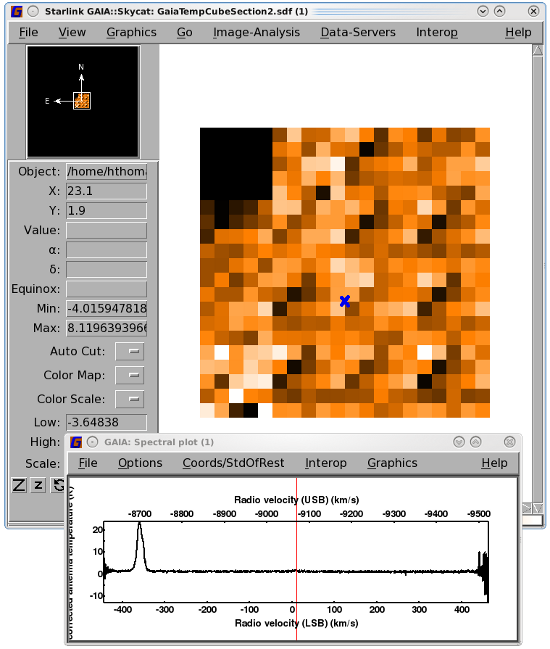
\includegraphics[width=0.65\linewidth]{sc20_makecubeout}
\typeout{sc20_makecubeout inserted on page \arabic{page}}
\caption[A regridded cube produced with \makecube.]{\label{fig:gaiareduced}
  The regridded cube displayed with \gaia. The 5$\times$5 jiggle
  pattern is evident in the map as is the missing receptor in the
  top-left corner. The smaller window shows the spectrum for the pixel
  selected by the blue cross on the map.}
\end{center}
\end{figure}

\subsection{Reducing multiple observations}

You can supply \makecube\ a group in a text file containing a list of
all the raw files you want reduced. These filenames should include the
full path if they are not in the local directory.

When you pass such group files to \makecube\ (and any \starlink\ command)
you should prefix the filename with an up-caret (\,\^\,).
\begin{terminalv}
% makecube in=^filelist.txt
\end{terminalv}

Alternatively you can use wild cards. The example below reads in all
the raw files for observation 10.
\begin{terminalv}
% makecube in=rawdata/a20140101_00010\*
\end{terminalv}


\section{Makecube Options}

\subsection{Specifying spectral bounds}

To save disk space and processing time you can specify the region of
the spectra to be processed with \param{SPECBOUNDS}. If you know your
line lies close to 0\kms, you may chose to process only the central
100\kms\ as in the example below.
\begin{terminalv}
%  makecube rawfile specbounds=\"-50.0 50.0\"
\end{terminalv}

\subsection{Masking receptors}

When combining several maps with masked bad receptors one can use the
\param{BADMASK} parameter of \makecube. This option determines the way
in which bad pixels are propagated from input to output. The one that
produces the best map is \param{badmask=and}, which uses all the data
so an output pixel will be bad only if all the input pixels that
contribute to it are bad. This generates an output map with the lowest
noise and fewest bad pixels. However, for large datasets the memory
requirements may be excessive.

Other options are \param{badmask=or} (default) and
\param{badmask=first}. \param{Or} means that an output pixel will be
bad if any of the input pixels that contribute to it are bad and is
the default.  The flag \param{first} means that the decisions on which pixels
will be flagged as bad will be made with the first input spectrum
while the rest are ignored.

\subsection{Including/excluding receptors}

To make a cube with only certain receptors you can use the
\param{detectors} option on the command line. This allows you to
either include or exclude specific receptors without the need for
masking. The example below makes a HARP map using all HARP 
receptors except H04 and H11.
\begin{terminalv}
% makecube in=rawfile autogrid out=map detectors=`"-H04,H11"'
\end{terminalv}
This alternative example makes a map using only receptor H10. Maps
made with single receptors may be used to evaluate the
receptor-to-receptor flat-field.
\begin{terminalv}
% makecube in=rawfile autogrid out=map detectors=`"H10"'
\end{terminalv}

When reduced by \makecube\ - either by hand or through the pipeline - it
is possible to find out which receptors are present in the data by inspecting the
reduced data file's FITS header. This can be done using \fitslist\ or fitsval and 
looking at the RECPUSED parameter.

\begin{terminalv}
% fitsval a20200808_00084_01_reduced001.sdf RECPUSED
NU0L NU1L
\end{terminalv}


\subsection{Defining an output grid}
\label{sec:outputgrid}
You can use the \param{REF} option to define an NDF which is used to
define an output grid. This NDF can even be in two dimensions even
though your data may be in three dimensions.
\begin{terminalv}
% makecube in=rawfile ref=myreffile
\end{terminalv}

If you do not supply a reference file \makecube\ will revert to the
\param{AUTOGRID} option.

If \param{autogrid=true}, the output grid is determined automatically
so that as many data samples as possible fall close to the centre of
pixels in the output cube.

If \param{autogrid=false}, \param{REFLON} and \param{REFLAT} are set to
the first pointing BASE position, \param{CROTA2} is set to the
\param{MAP\_PA} value in the FITS header (converted to the requested
sky co-ordinate system), PIXSIZE is set to 6 arcseconds, and
\param{REFPIX1} and \param{REFPIX2} are both set to zero. See
\smurfsun\ for a full description of each of these parameters.

\subsection{Data-regridding options}
\label{sec:gridding}

There are several regridding options available to you through the
\makecube\ command. These are specified with the \param{SPREAD}
parameter on the command line.  For instance,
\begin{terminalv}
% makecube in=rawfile spread=sincsinc params="[6,9]"
\end{terminalv}

The default method is \param{Nearest}, which assigns the input pixel
completely to the nearest output pixel. This is the fastest method
available but is not optimal. In particular it may result in blank
pixels in HARP maps due to missing receptors (see
\cref{Figure}{fig:spread}{}).

%If \param{spread=nearest} you can supply a value for the
%\param{BADMASK} option. This determines the way in which bad pixels
%are propagated from input to output. The default is
%\param{badmask=AND} which uses all data and results in the best map
%,however it requires considerable memory so the alternatives are FIRST
%and OR. See \smurfsun\ for more details.

We recommend you select one of the other methods available which
spread the emission to neighbouring pixels.  These include
\param{Gauss} and \param{SincSinc} which are the most common, although
the latter sometimes gives noisy edges with negative values in some
pixels. \param{SincCos} will give neater edges. For each of these you
will need to provide the size of the convolution function through the
\param{params} option as in the example above. See \smurfsun\ for more
details.


\begin{figure}[h!]
\begin{center}
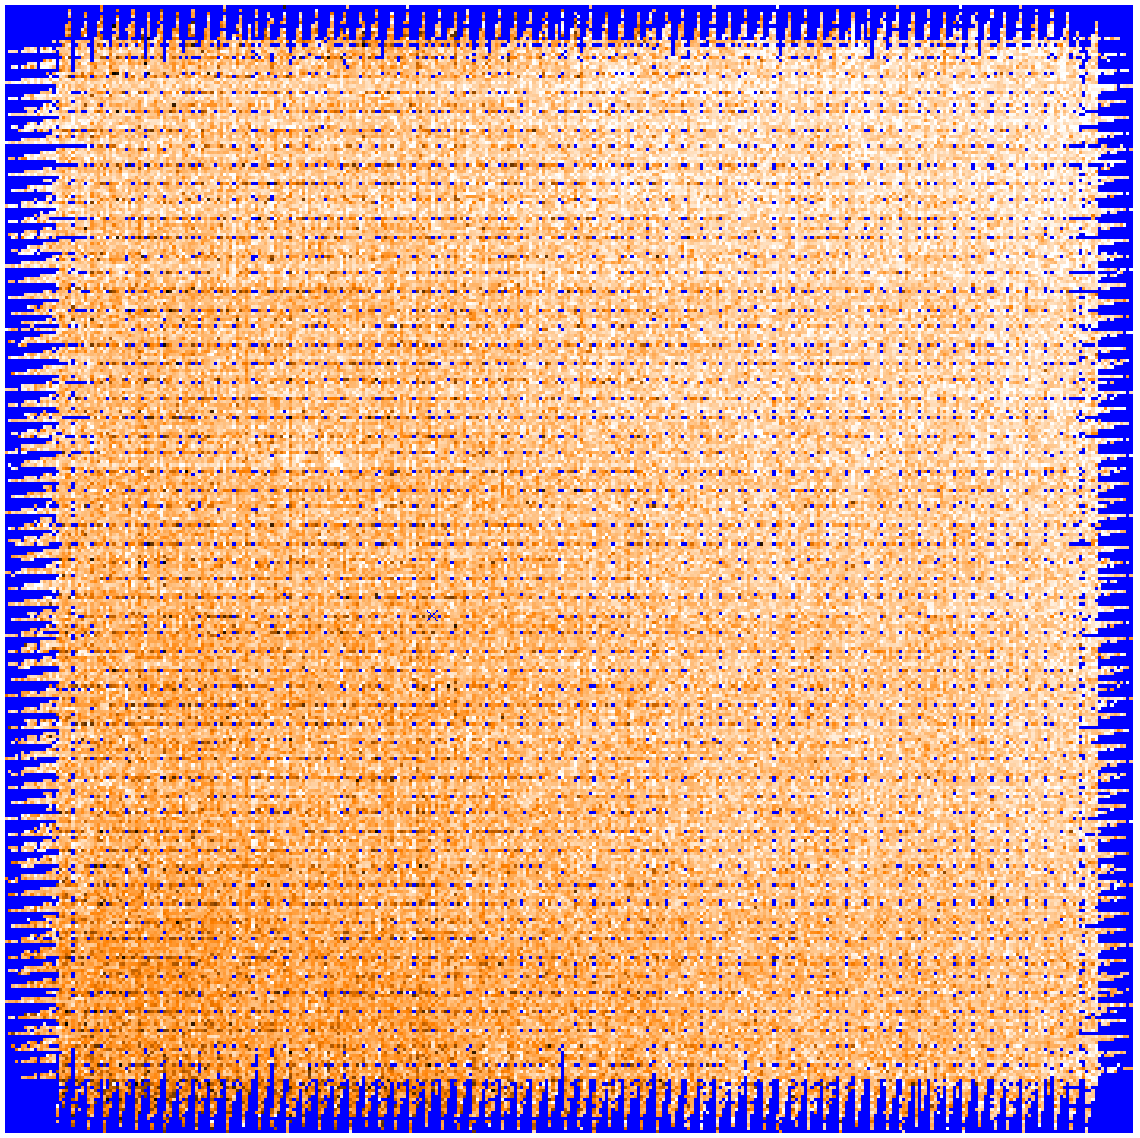
\includegraphics[width=5.2cm, height=5.2cm]{sc20_nearest}
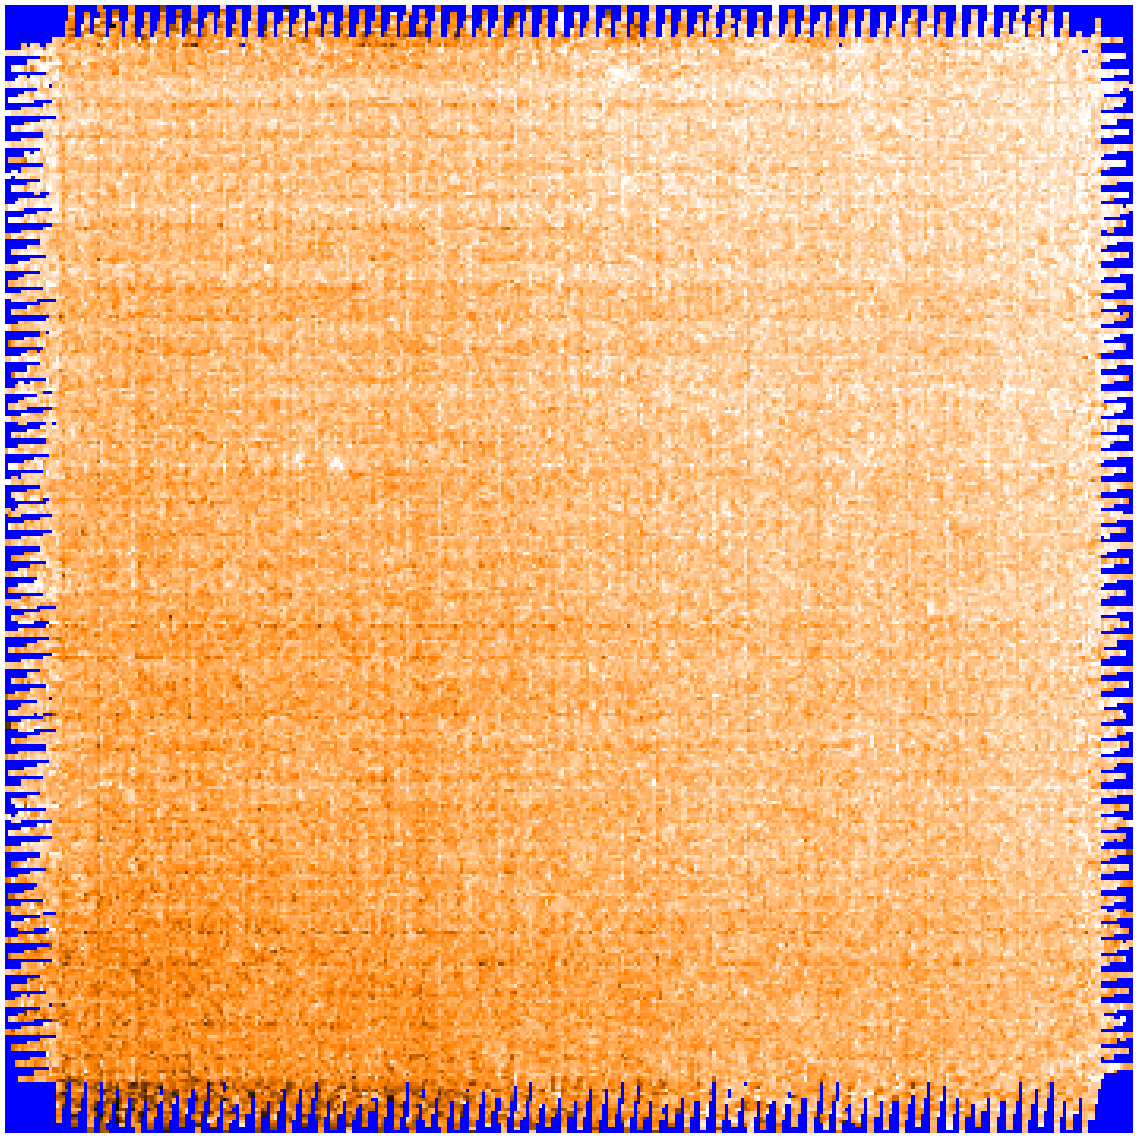
\includegraphics[width=5.2cm, height=5.2cm]{sc20_gauss}
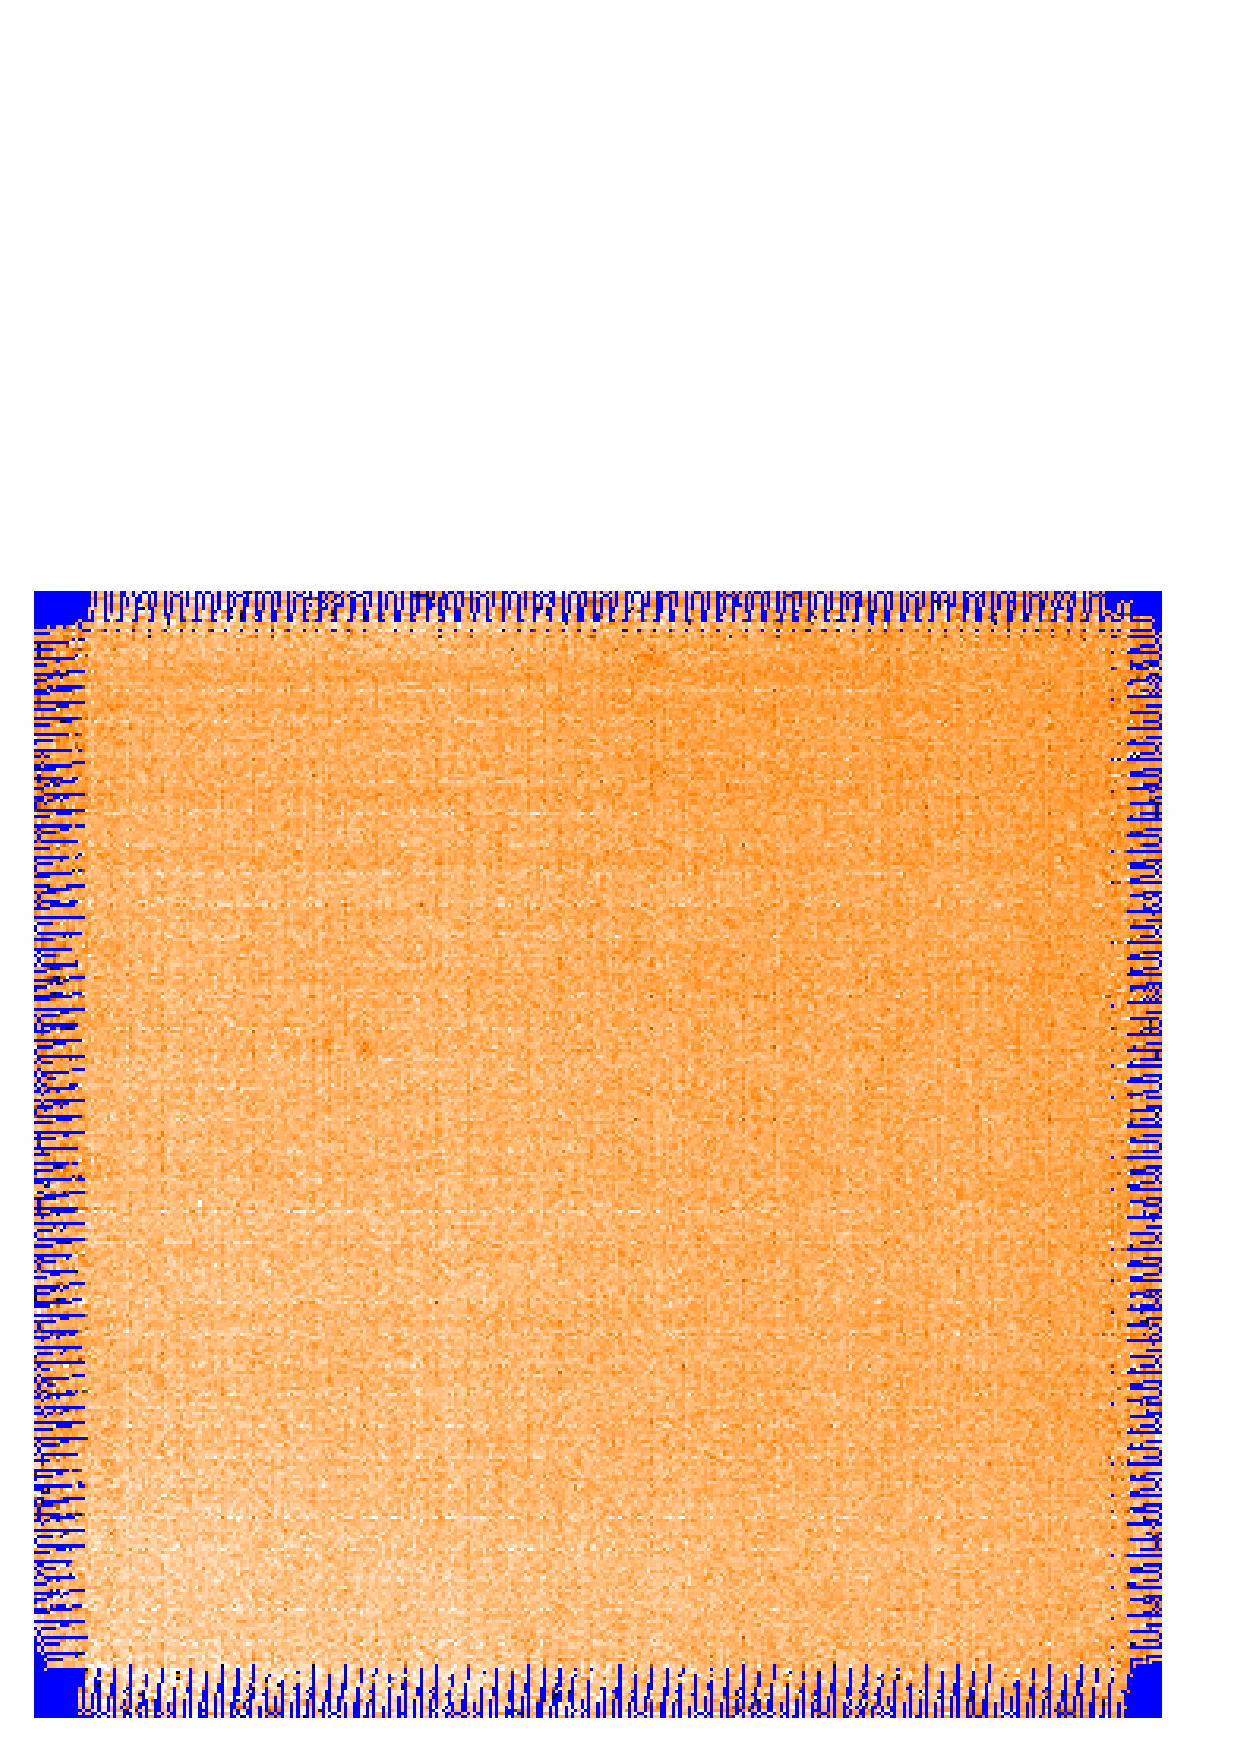
\includegraphics[width=5.2cm, height=5.2cm]{sc20_sincsinc}
\caption[Options for the \makecube\ parameter `spread']{\label{fig:spread}
  Raster map regridded with \makecube\ and \param{spread = nearest}
  (left), \param{Gauss} (centre) and \param{SincSinc} (right). Blank
  pixels are coloured blue. You can see the Nearest option has
  resulted in multiple blank pixels throughout the map.}
\end{center}
\end{figure}


\subsection{Generating a variance map}

The option \param{GENVAR} can be used to generate a variance array for
your cube. This is important if you are adding multiple maps with
different variances as it allows them to be accurately weighted. There
are three options for \param{GENVAR}:

\begin{center}
\begin{aligndesc}
\item[\textbf{Spread }]
The output variance values are based on the spread of input data
values contributing to each output pixel. Note that this option is not
available if parameter \param{SPARSE} is set \param{true}. If the
\param{BADMASK} value is \param{or} or \param{first}, then a single
variance value will be produced for each output spectrum. However,
when \param{BADMASK} is \param{and}, an independent variance value is
calculated for each channel in each output spectrum.
\vspace{0.7cm}\\
\item[\textbf{Tsys }]
The output variance values are based on the system noise temperature
values supplied in the input NDFs. Since each input spectrum is
characterised by a single Tsys value, each output spectrum will have a
constant variance value (i.e. all channels in an output spectrum will
have the same variance value). [Default].
\vspace{0.7cm}\\
\item[\textbf{None }]
 No output variance values are created.\\
\end{aligndesc}
\end{center}

\subsection{Sparse grid}

If one has observed a number of offset positions which are not on a
regular grid or are widely spaced, it is of little use to make a
normal cube with \makecube, which then would have a large size and
which would be mostly empty. Then one can use the \makecube\ parameter
\param{SPARSE}. When \param{sparse=true} a one-dimensional array is
created which stacks spectra in the order in which they were observed
(from left to right when viewed with \gaia).
\begin{terminalv}
% smurfhelp makecube param sparse
\end{terminalv}
This is generates a one-dimensional array where spectra are displayed by
\gaia\ in the order where they were observed (from left to right).

\subsection{Creating a catalogue of receptor positions}

You can use the option \param{OUTCAT} to generate a catalogue of the
spatial positions of the receptors used to make your final cube. The
label associated with each row in the catalogue is the detector name.
The detector positions in the catalogue are ordered as follows: all
the positions for the first input NDF come first, followed by those
for the second input NDF, etc. Within the group of positions
associated with a single input NDF, the positions for the first time
slice come first, followed by the positions for the second time slice,
and so on.

\begin{terminalv}
% makecube in=rawfiles outcat=cat
\end{terminalv}

The catalogue produced will be in FITS format. In the example above a
file called \file{cat.FIT} is created. When viewing your map with \gaia\ this
catalogue can be overlaid to identify the receptors contributing to
each pixel (see \cref{Figure}{fig:makecube-outcat}{}).

\begin{figure}[h!]
\begin{center}
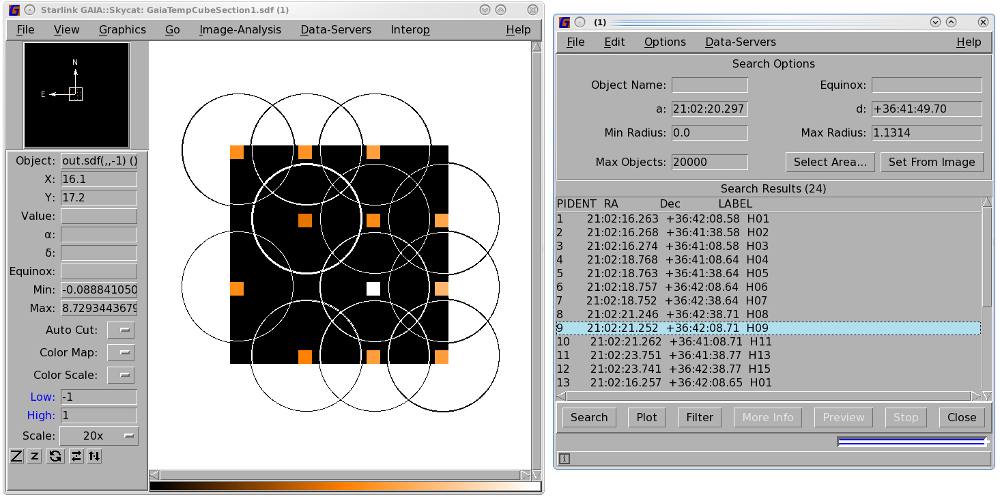
\includegraphics[width=1\linewidth]{sc20_makecube-outcat}
\typeout{sc20_makecube-outcat inserted on page \arabic{page}}
\caption[Displaying receptor positions in \gaia.]{\label{fig:makecube-outcat}
  The receptor positions overlaid on a regridded cube of a HARP stare
  observation. This is viewed in \gaia\ by selecting
  \guithing{Data-Servers} $>$ \guithing{Local Catalogs} and selecting
  your \param{OUTCAT} filename (here \file{cat.FITS}). Notice that dead
  receptors are excluded from the list.}
\end{center}
\end{figure}

\subsection{Tile dimensions}

For large data sets, it may be beneficial to break the output array up
into a number of smaller rectangular tiles. This can be controlled by
the \param{TILEDIMS} parameter.  The files can be stitched together
later using the \Kappa\ application \paste\ which may be used any time
the tiles to be abutted have the same pixel co-ordinates.  Each tile
may also have a rim of extra data to allow for future co-adding,
the width of which is set by the \param{TILEBORDER} parameter.


\clearpage
\chapter{\xlabel{analyse}Analysing your Cube}
\label{sec:analyse}

\section{Smoothing your data}

Frequency or velocity smoothing is performed using \Kappa:\block. It
uses a rectangular box filter with each output pixel either the mean
or the median of the input pixels within the filter box. The box size
can be set to 1 for dimensions which do not require smoothing. In the
example below the spatial pixels remain untouched while the velocity
axis is smoothed using a box of five channels.
\begin{terminalv}
% block in=mycube out=rebinnedcube box="[1,1,5]"
\end{terminalv}

Two-dimensional NDFs can also be smoothed using \gausmooth. This
smooths using a symmetrical Gaussian point spread function (PSF) of
specified width(s) and orientation. Each output pixel is the
PSF-weighted mean of the input pixels within the filter box.

\begin{terminalv}
% gausmooth in=mymap out=smoothedmap fwhm=3
\end{terminalv}
Note that the \param{fwhm} option is given in the number of pixels.
For example, to smooth a map with 4\arcsec pixels by a 12\arcsec Gaussian
you would set \param{fwhm=3}.

\section{Removing a baseline}

Baselines can be removed using \Kappa:\mfittrend. This routine can
fit polynomials up to order 15, or cubic splines, to each spectrum in
your cube. You can specify the ranges to fit via the \param{ranges}
parameter, or you can allow them to be determined automatically
(\param{auto}), say if the number of observations is large.

\begin{terminalv}
% mfittrend in=cube ranges=\"-50 -10 80 160\" order=1 axis=3 out=baselinedcube
\end{terminalv}

If using automatic range determination you should set the
\param{numbin} option. This is the number of bins in which to compress
the trend line. A single line or average may be noisy so binning is
used to improve the signal-to-noise in order to enhance features that
should be masked.

Ideally the bin size should match your line width to get maximum
single to noise between the emission and the background. Be aware that
bins that are too big can dilute weaker features. Likewise, bins that
are too small will get noisy at the edges of broad lines. We recommend
you experiment with the bin size to find the best fit for your data.

To exclude features that are not part of the baseline trend you can
use the \param{clip} option. Use \param{clip} to provide an array of
standard deviations for progressive clipping of outliers within each
bin. Once the data have been binned a trend is fit within each bin and
the outliers clipped, the trend is then re-fitted and the outliers
again clipped etc. By default this will clip at 2, 2, 2.5 and
3\,$\sigma$ successively but you may wish to experiment with your own
clip levels. The \param{clip} option is only used when
\param{auto=true}.

For convenience \gaia\ has a \guithing{Baseline} tab in its cube
control panel---see \cref{Section}{sec:gaiabaseline}{Removing a
baseline with GAIA} for an example.  This invokes \mfittrend.


\subsection{Advanced method}
These steps give a more in depth way of determining the baselines and
mimic the pipeline.

\begin{enumerate}[label=(\arabic*)]
\item Perform a \block\ smooth on your reduced cube. Here the
smoothing is quite aggressive with a box filter of five pixels along the
spatial axes and fifteen pixels along the frequency axis. This is to really
pull out all emission features. You can tweak these to suit your data,
e.g a narrower box might be needed if you have very narrow lines.
\begin{terminalv}
% block in=cube out=temp1 box="[5,5,15]" estimator=mean
\end{terminalv}

\item Perform \mfittrend\ on your smoothed cube with a high-order
polynomial and automatic range determination.
\begin{terminalv}
% mfittrend in=temp1 out=temp2 axis=3 order=3 auto method=single \
  variance subtract=false mask=blmask
\end{terminalv}

\item Add the baseline mask to your original unsmoothed cube.
\begin{terminalv}
% add in1=cube in2=blmask out=temp3
\end{terminalv}

\item Perform \mfittrend\ on your masked unsmoothed cube with a
lower-order polynomial. This time fit the full range by setting
\param{auto=false}.
\begin{terminalv}
% mfittrend in=temp3 out=temp4 axis=3 order=1 auto=false ranges=\! \
  method=single variance=true subtract=false
\end{terminalv}

\item Subtract the baseline from the original unsmoothed cube.
\begin{terminalv}
% sub in1=cube in2=temp4 out=baselinedcube
\end{terminalv}
\end{enumerate}

\subsection{What about \findback?}

The \cupid\ routine \findback\ offers an alternative for background
subtraction however there are more limitations. It applies spatial
filtering to remove structure with a size scale less than a specified
box size. Within each box the values are replaced by the minimum of
the input values. The data are then filtered again and this time
replaced with the maximum in each box.

Using \findback\ results in a baseline trend that hugs the lower limit
of the noise and can contain sharp edges. These problems can be
mitigated but extra steps are required. See \cupidsun\ for more
details.

\section{Collapsing your map}

An integrated intensity map can be created by collapsing your cube
along the frequency/velocity axis using \Kappa:\collapse. For each
output pixel, all input pixels between the specified bounds are
collapsed and combined using one of a selection of estimators. Amongst
others, the estimators include the mean, integrated value, maximum
value, the mean weighted by the variance, RMS value and total value.
See \kappasun\ for a full list.

The example below includes the options \param{low} and \param{high}
which can be specified to limit the range over which the cube is
collapsed on the given axis (in this case from $-5$\kms\ to $+10$\kms).
The \param{variance} flag indicates the variance array should be used
to define weights and generate an output variance. The option
\param{wlim} sets the fraction of pixels that must be `good' in the
collapse range for a valid output pixel to be generated. You may find
you need to reduce the value for \param{wlim} below its default of 0.3
for some data.

\begin{terminalv}
% collapse in=cube axis=vrad estimator=integ variance=true low=-5.0 high=10.0 \
  wlim=0.5 out=integmap
\end{terminalv}
If you do not know the axis name you can give the number instead
(1=RA, 2=Dec, 3=vrad).

For convenience \gaia\ has a \guithing{Collapse} tab in its cube
control panel---see \cref{Section}{sec:gaiacollapse}{Collapsing your
cube with GAIA} for an example.  This invokes \collapse.


\subsection{Advanced method}

These steps mimic the pipeline and show the procedure for generating
an integrated map collapsed only over regions with emission greater
than 3\,$\sigma$.

\begin{enumerate}[label=(\arabic*)]
\item Use \findclumps\ to run a clump-finding algorithm on your cube.
Specify the 3\,$\sigma$ limit in your configuration file. See Section
\ref{sec:clumpfind} for more details on clump-finding and Section
\ref{sec:noise} for how to determine your RMS.
\begin{terminalv}
% findclumps in=cube rms=<medianrms> config=^myconfig.dat \
  method=clumpfind out=temp1 outcat=mycat deconv=no
\end{terminalv}

\item Divide the map by itself to create a clump mask that has clump
regions set to 1.
\begin{terminalv}
% div in1=temp1 in2=temp1 out=temp2
\end{terminalv}

\item Set the bad data to zero using \Kappa:\nomagic.
\begin{terminalv}
% nomagic in=temp2 out=temp3 repval=0
\end{terminalv}

\item Multiply your reduced cube by the clump mask.
\begin{terminalv}
% mult in1=cube in2=temp3 out=maskedcube
\end{terminalv}

\item Collapse your masked reduced cube.
\begin{terminalv}
% collapse in=maskedcube out=integ estimator=integ wlim=0.1 variance
\end{terminalv}
\end{enumerate}

\subsection{Moments Maps}

You can use \collapse\ to generate the moments maps by selecting the
appropriate \param{estimator} option---Integrated value
(\param{Integ}) for the integrated map (zeroth moment),
Intensity-weighted co-ordinate (\param{Iwc}) to get the velocity field
(first moment), or Intensity-weighted dispersion (\param{Iwd}) to get the
velocity dispersion (second moment).

\begin{tip}
TIP: You can also use the \picard\ recipe CREATE\_MOMENTS\_MAPS. See
\cref{Appendix}{app:picard}{Picard} for details. This recipe follows
the advanced method outlined above.
\end{tip}


\section{\xlabel{tempscale}Temperature scales}
\label{sec:mult}

Your cube will come out of \makecube\, and the pipeline, in units of
$T_{\textnormal{A}}^*$. To convert this to main-beam brightness temperature, $T_{\textnormal{MB}}$
divide your cube by the main-beam efficiency, $\eta_{\textnormal{MB}}$. Alternatively,
to convert to receiver temperature, $T_{R^{*}}$, divide by the forward
scattering and spillover efficiency, $\eta_{\textnormal{\,fss}}$.  See
\cref{Section}{sec:instruments}{Heterodyne instruments} for efficiency
values for RxA and HARP, and the JCMT webpages for further information
and historical numbers.

You can use the \Kappa\ command \cdiv\ to divide any NDF by a constant.

\begin{terminalv}
% cdiv in=harpcube scalar=0.63 out=harpcube_Tmb
\end{terminalv}

\section{\xlabel{rebin}Changing the pixel size}
\label{sec:rebin}

You may want to \htmlref{\emph{regrid}}{app:regrid} your data onto
larger pixels, for instance to
allow direct comparison with data from other observatories. In the
example below a JCMT map is regridded and aligned to match a Herschel
map. See \cref{Appendix}{app:convert}{Converting file formats} for
instructions on converting your FITS file to NDF format.
\begin{terminalv}
% wcsalign in=jcmtmap out=regridmap lbnd=! ubnd=! ref=herschelmap rebin conserve=f
\end{terminalv}

Alternatively, to \htmlref{\emph{resample}}{app:regrid} your data onto smaller
pixels you should
use the \Kappa\ command \sqorst. In the example below 'map' has a
pixel size of 8\arcsec, while `resamplemap' has a pixel size of 4\arcsec --
the number of pixels has been doubled by applying a factor of 2 to the
spatial axes. A factor of 1 was applied to the frequency (third) axis
leaving it unchanged.
\begin{terminalv}
% sqorst in=map out=resamplemap factors="[2,2,1]" conserve
\end{terminalv}
\param{mode=factors} is the default setting so it was not specified in
the example above. The example below however, uses
\param{mode=pixelscale} to define a pixel size for the third axis;
here the spectra are rebinned into 2\kms\ channels.
\begin{terminalv}
% sqorst in=map out=resamplemap mode=pixelscale pixscale=2 axis=3
\end{terminalv}

Remember you can check your current pixel size and channel spacing
with \ndftrace\ (see \cref{Section}{sec:fitslist}{How can I view the
metadata?}).

\section{\xlabel{mosaic}Mosaicking cubes}
\label{sec:mosaic}

If you pass raw files covering different regions of the sky to
\makecube\ it will automatically mosaic them together. This can be
heavy work for your processor so you may wish to make individual cubes
and combine them during post-processing. To co-add multiple reduced
maps you should use \wcsmosaic.

Note that this is not the same as stitching the tiles of a reduced cube
from a single \makecube\ command.  Such tiles share common pixel
co-ordinates and so can be combined with \paste\
(\cref{Section}{sec:multireduced}{why have multiple reduced files been
generated?}). Separately created
cubes will not have the same pixel co-ordinates, and therefore the
world co-ordinates are required to align the tesserae in the mosaic of
an extended region.

\begin{terminalv}
% wcsmosaic in=^maplist out=mosaic lbnd=! ubnd=! variance
\end{terminalv}
By selecting the lower bound (\param{lbnd}) and upper bound
(\param{ubnd}) to be default (!) you are including all of the input
tiles. You can change these if you want to only mosaic a sub-region of
the input maps. As with \makecube\ there are a number of regridding
options available to you describing how to divide an input pixel
between a group of neighbouring output ones (the default is
\param{SincSinc}).

Note that by default \wcsmosaic\ aligns reduced cubes along the
spectral axis using the heliocentric standard of rest (the \ORACDR\
pipeline also does this).  If you want to align using
a non-heliocentric standard of rest, you should set the
\att{AlignStdOfRest} attribute for your NDFs using \wcsattrib\
before running \wcsmosaic.
The following example sets the alignment to the kinematic LSR.

\begin{terminalv}
% wcsattrib <list_of_separate_cubes> set AlignStdOfRest LSRK
\end{terminalv}

where $<$list\_of\_separate\_cubes$>$ is group of cubes specified
as a comma-separated list or as one per line in a text file.

\begin{tip}
Take care not to combine data separated on the sky as \wcsmosaic\
will attempt to create a vast cube that encompasses all the input
files until it runs out of resources.
\end{tip}

\begin{tip}
You can also use the \picard\ recipe MOSAIC\_JCMT\_IMAGES. This
will correctly combine all NDF extensions. See
\cref{Appendix}{app:picard}{Picard} for details.
\end{tip}

\newpage
\section{\xlabel{Crop}Cropping your map}
\label{sec:collapse}

Cropping an ACSIS map can be fiddly. The simplest way is to create an
ARD mask in \gaia\ and apply it to your map. The steps below work on
both two- and three-dimensional data.

\begin{enumerate}[label=(\arabic*)]
\item Create your ARD mask. You may find it easiest to do this with
\gaia. See \cref{Figure}{fig:ardmask}{} for an illustrated guide.

\item Trim off the third axis from your mask using \ndfcopy.
\begin{terminalv}
% ndfcopy mask trim trimwcs
\end{terminalv}

\item Apply the saved ARD mask to your map. Setting
\param{inside=false} will mask the pixels outside rather than inside
your mask. The masked pixels will appear blank when you open it with
\gaia; see the left-hand panel of \cref{Figure}{fig:crop}{}.
\begin{terminalv}
% ardmask map inside=false ard=ardmask.txt out=maskmap
\end{terminalv}

\item Trim off the blank pixels using \ndfcopy\ with the
\param{trimbad} option. This leaves just your selected region; see the
right-hand panel of \cref{Figure}{fig:crop}{}.
\begin{terminalv}
% ndfcopy maskmap trimbad
\end{terminalv}
\end{enumerate}

An alternative method is to use \ndfcopy\ while defining the section
of the map or cube you wish to extract as an output cube. See
\cref{Section}{sec:ndfsections}{How to examine, process or extract a
subset of your data}.

\subsection{Supplying a template}

If you wish to extract only a region which overlaps with an existing
file you have, e.g. from a different observing campaign or telescope,
you can also use \ndfcopy\ but with the \param{like} option.
\begin{terminalv}
% ndfcopy in_full out_cropped like=map2 likewcs
\end{terminalv}
The shape of the file supplied by \param{like} will determine the
shape of the output file. This shape can be in either pixel indices or
the current WCS Frame. If the WCS Frame is required, include the
parameter \param{likewcs} to the command line otherwise it can be
omitted.


\begin{figure}[ht!]
\begin{center}
\begin{fmpage}{0.99\linewidth}
\vspace{0.2cm}
\hspace{0.2cm}
\textbf{Defining an ARD region in \gaia}

\vspace{0.5cm}
\hspace{0.1cm}
\begin{minipage}[c]{0.23\linewidth}
Open your map with \gaia.
\end{minipage}
\hspace{0.2cm}
\begin{minipage}[c]{0.72\linewidth}
\begin{terminalv}
% gaia map
\end{terminalv}
\end{minipage}

\begin{minipage}[c]{1.0\linewidth}
\end{minipage}

\vspace{0.5cm}
\hspace{0.1cm}
\begin{minipage}[c]{0.23\linewidth}
In \gaia\ go to \guithing{Image-analysis$>$Image regions}.
\end{minipage}
\hspace{0.2cm}
\begin{minipage}[c]{0.72\linewidth}
\centering
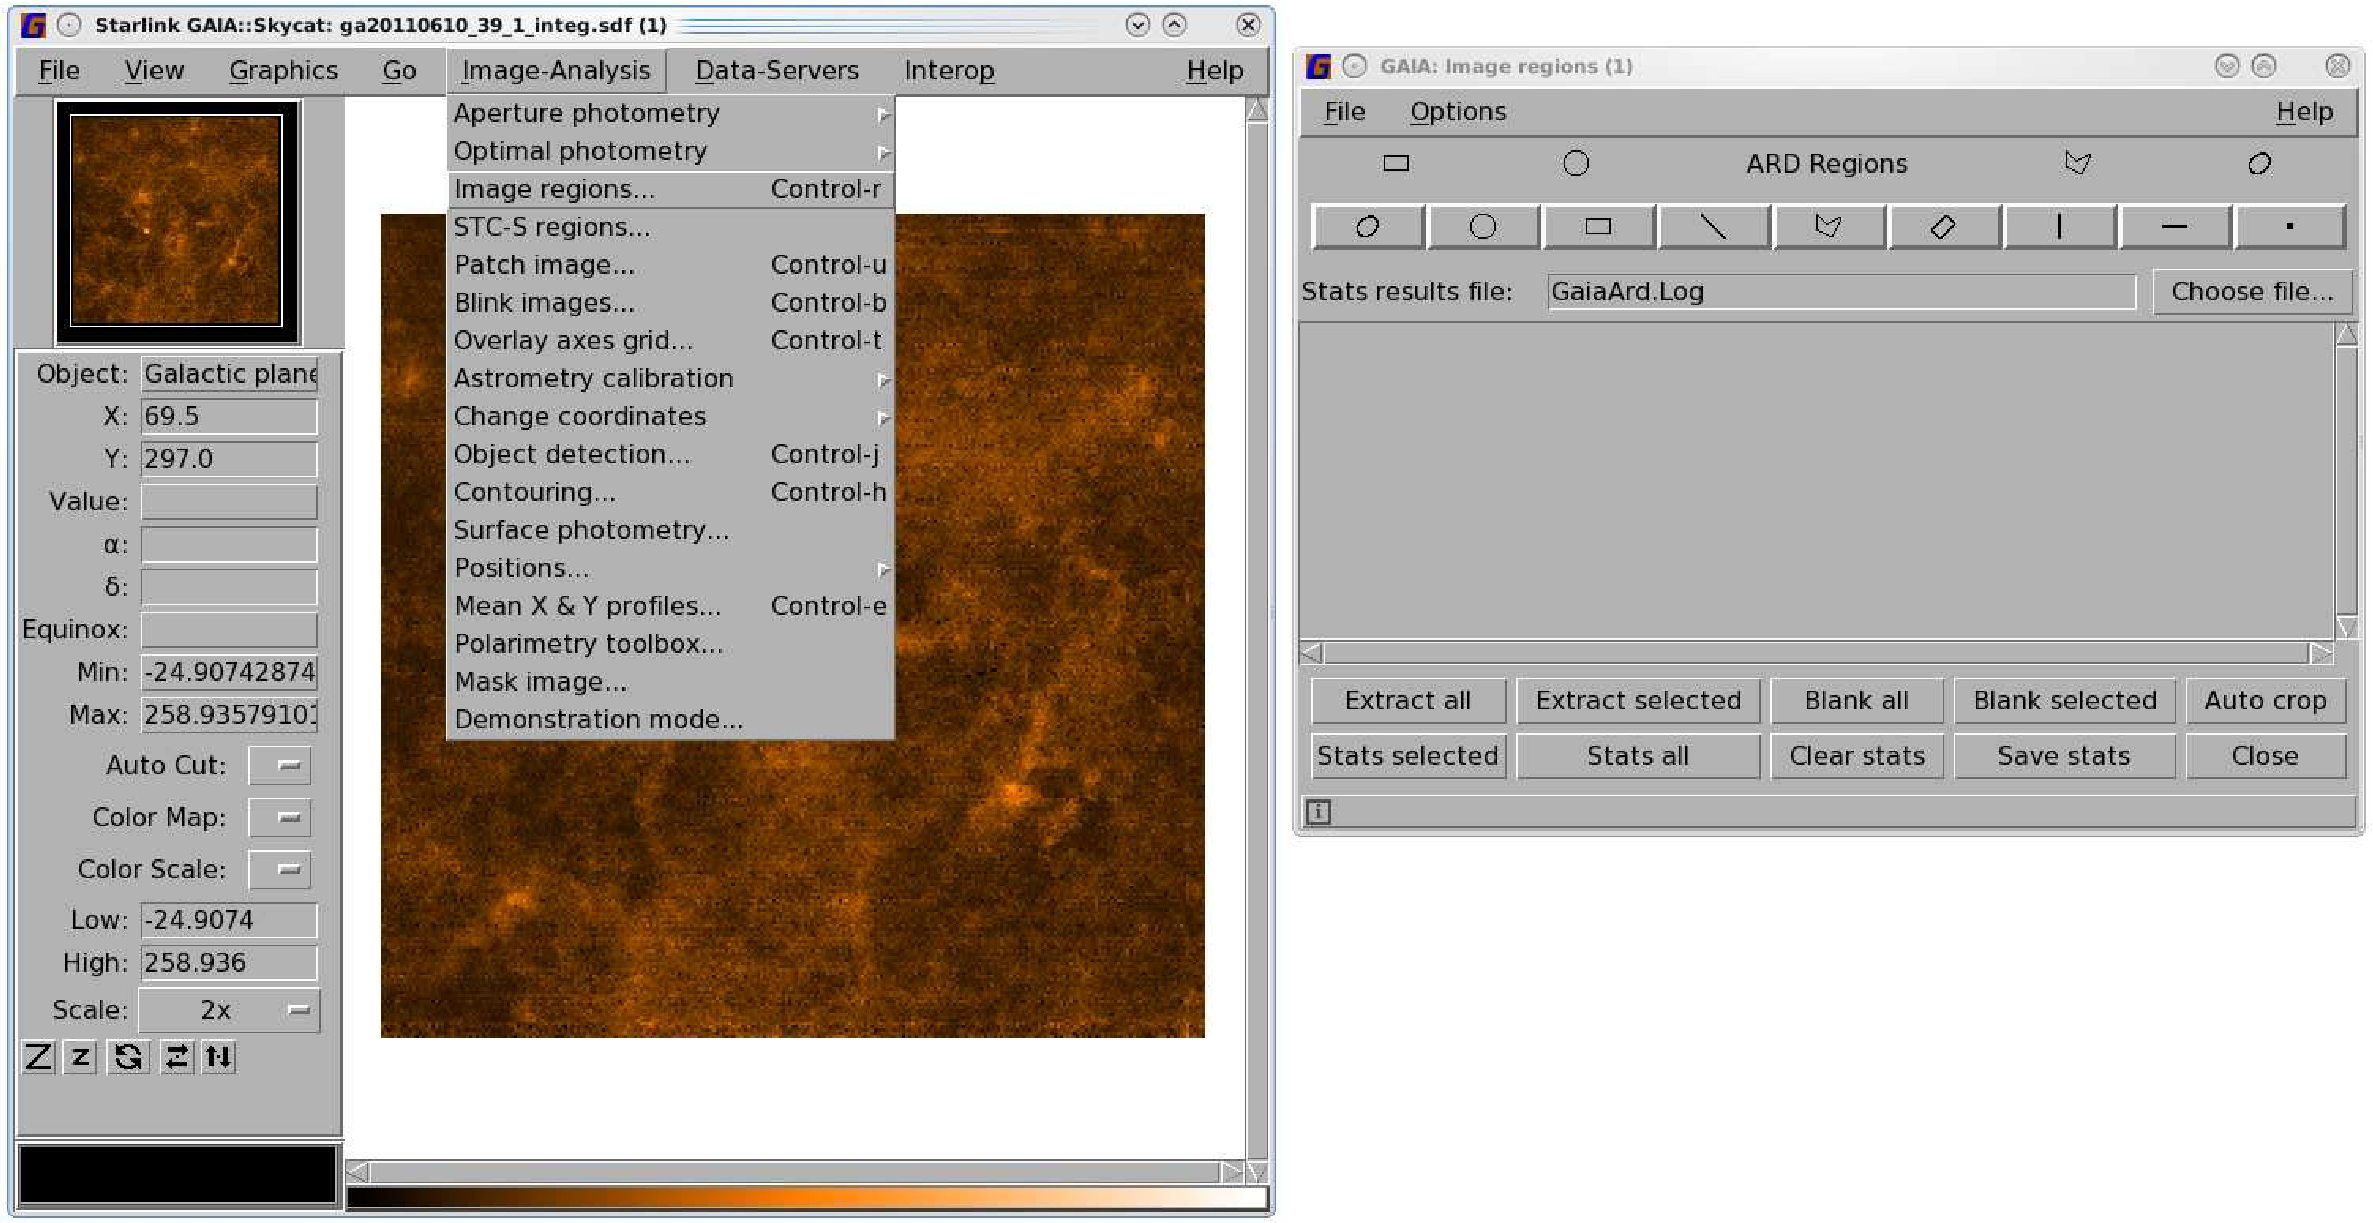
\includegraphics[width=0.98\textwidth]{sc20_ard7}
\end{minipage}

\vspace{0.5cm}

\hspace{0.1cm}
\begin{minipage}[c]{0.23\linewidth}
Select the shape of the ARD region you wish to define and drag it on
your map by holding the mouse button down, dragging the shape out,
then releasing the button.
\end{minipage}
\hspace{0.2cm}
\begin{minipage}[c]{0.72\linewidth}
\centering
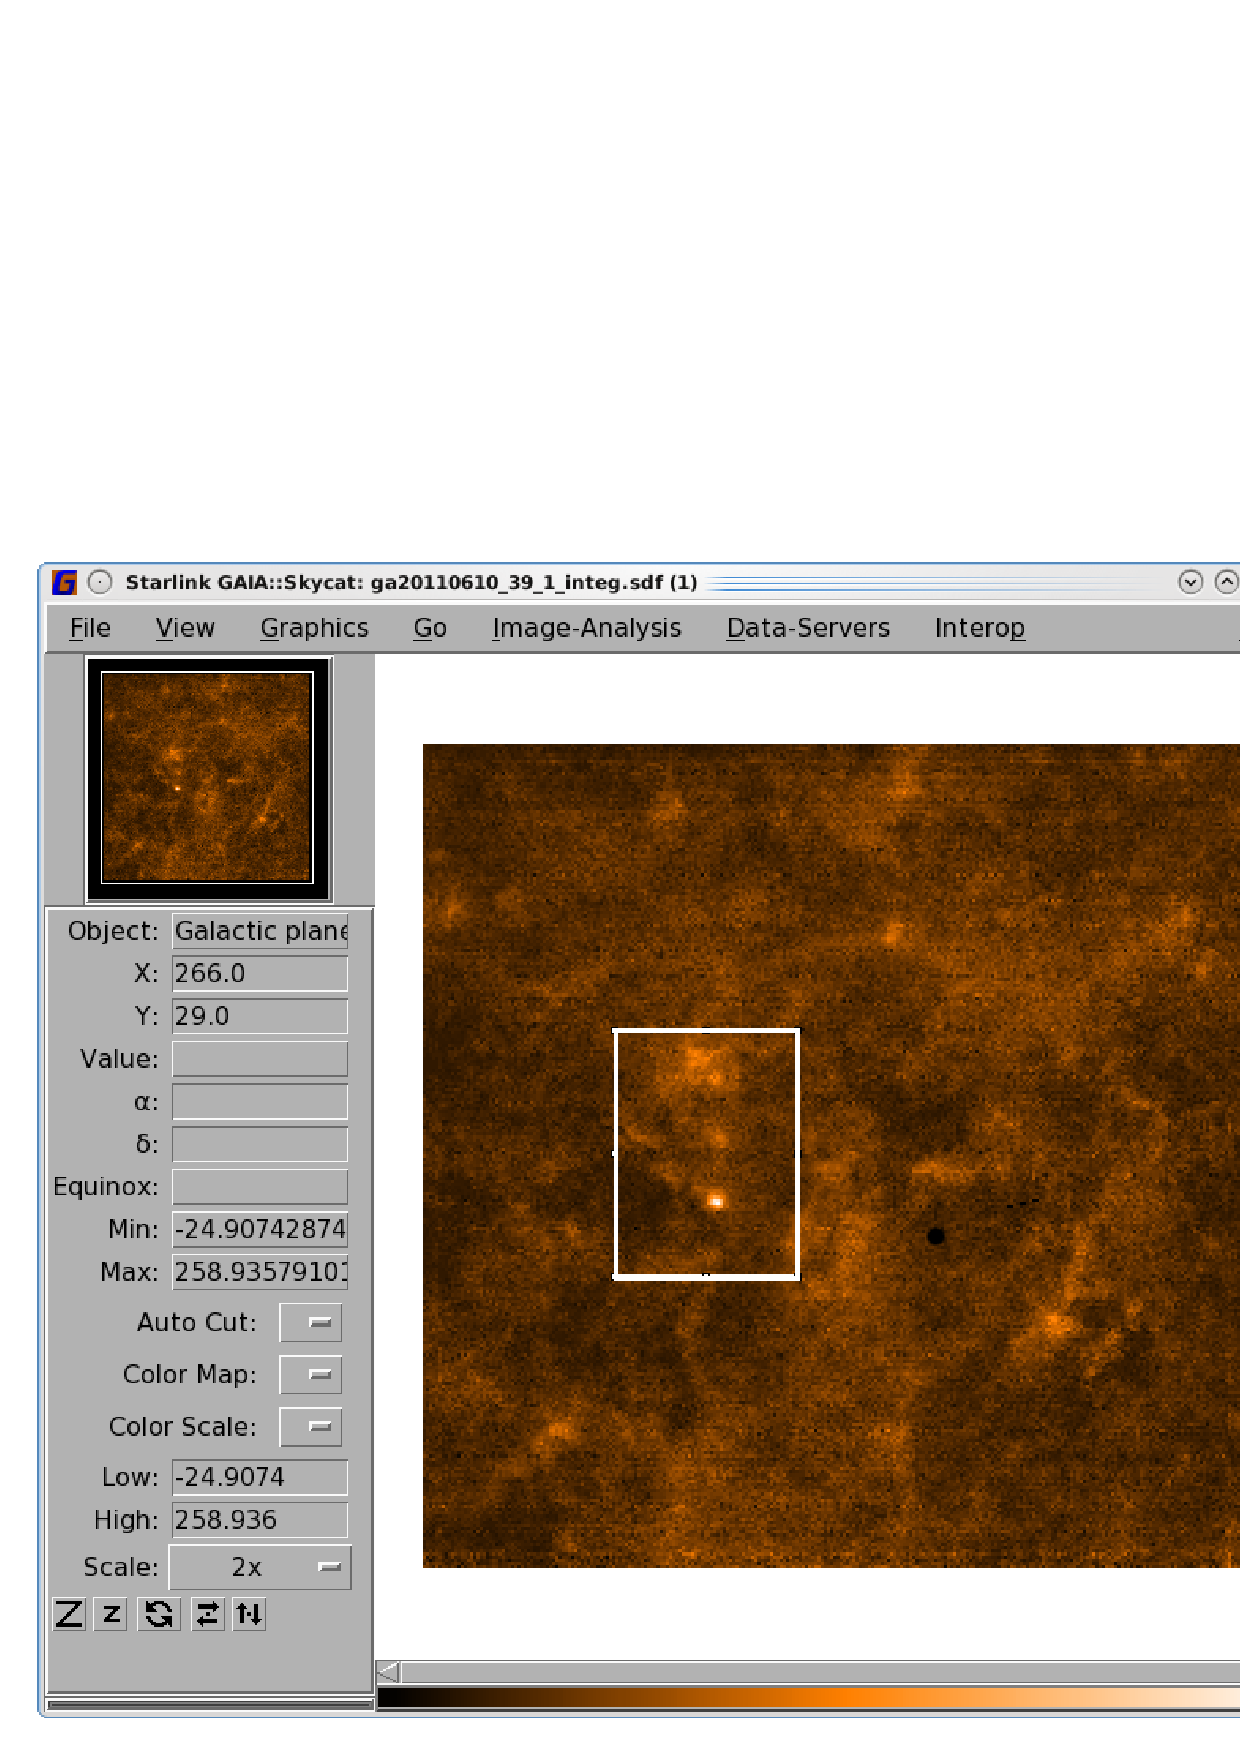
\includegraphics[width=0.98\textwidth]{sc20_ard3}
\vspace{0.2cm}
\end{minipage}

\vspace{0.5cm}


\hspace{0.1cm}
\begin{minipage}[c]{0.23\linewidth}
In the \guiwindow{Image regions} window go to \guithing{File$>$Save
ARD description} to save your ARD mask for later use.
\end{minipage}
\hspace{0.2cm}
\begin{minipage}[c]{0.72\linewidth}
\centering
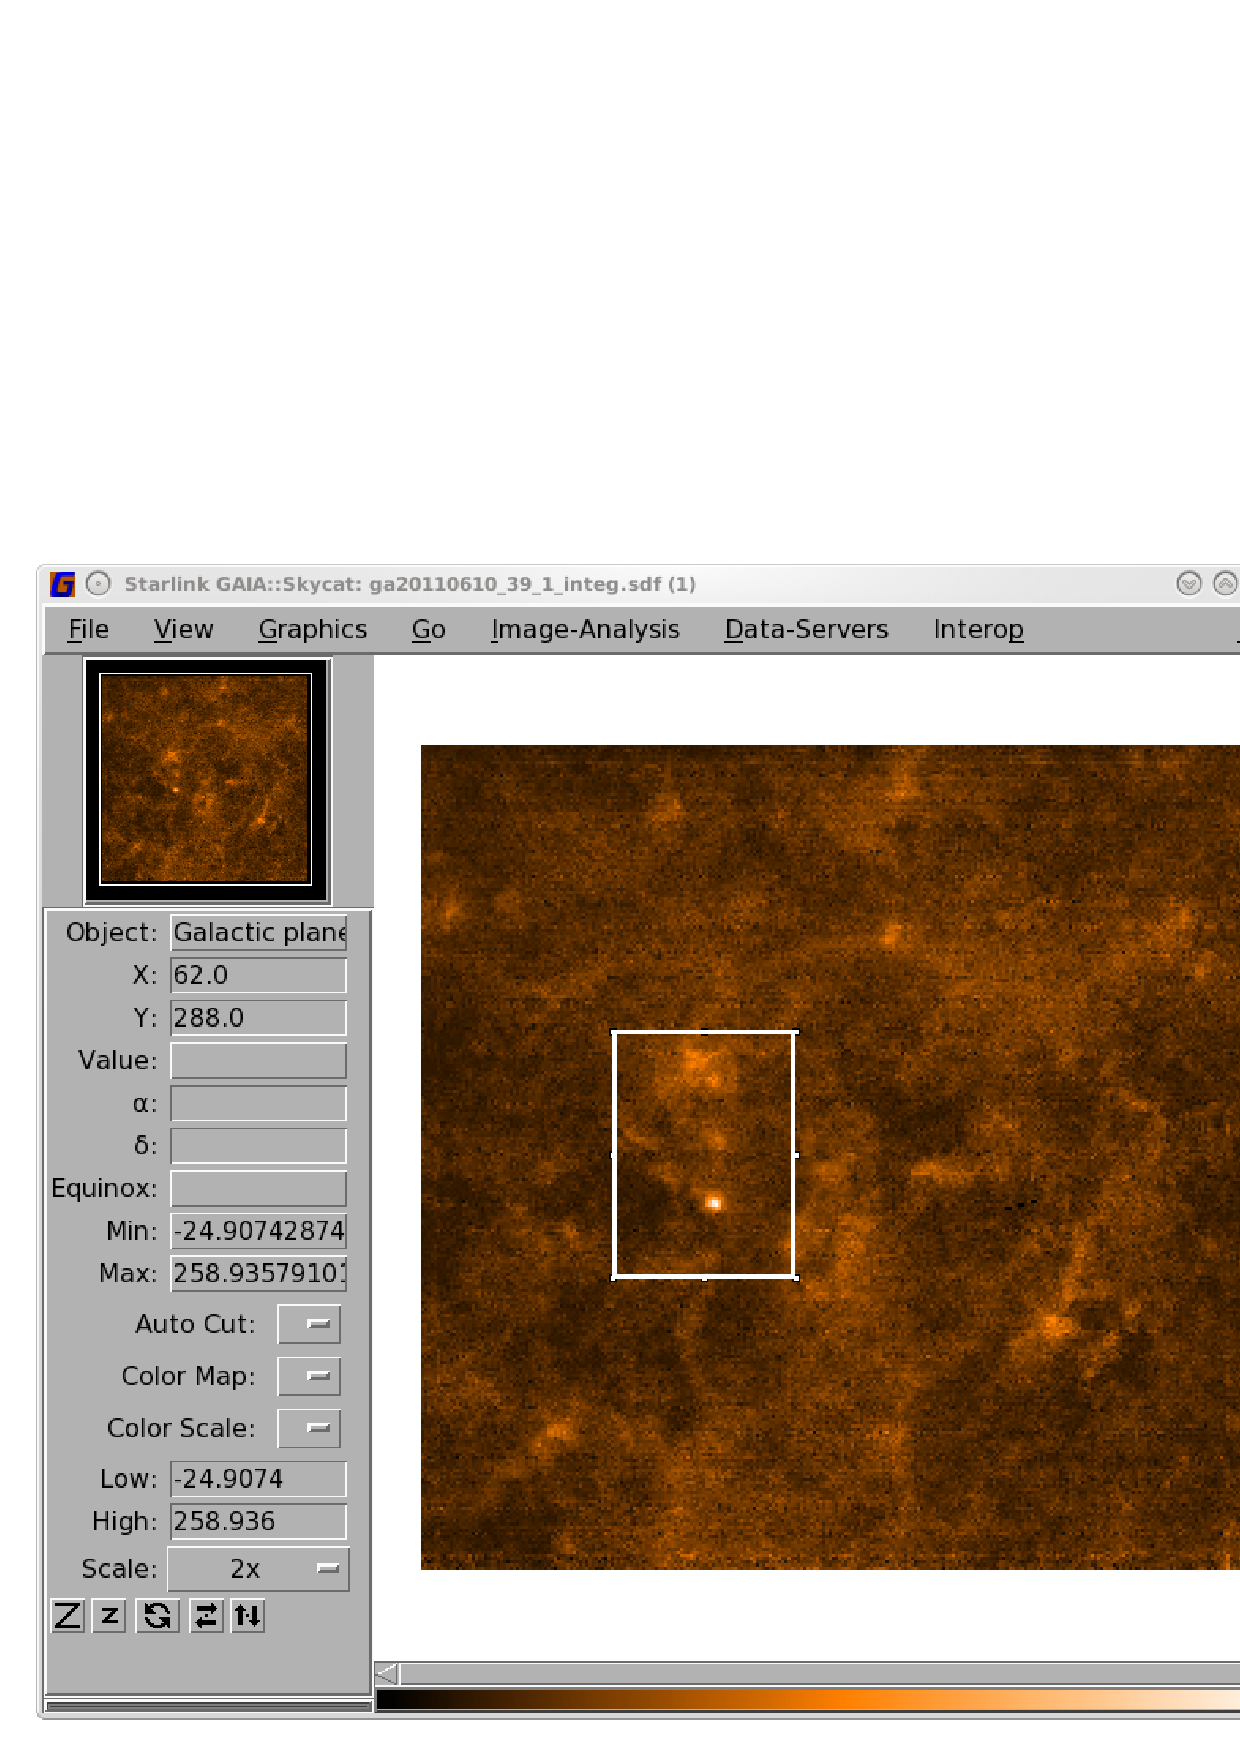
\includegraphics[width=0.98\textwidth]{sc20_ard4}
\vspace{0.2cm}
\end{minipage}

\end{fmpage}
\end{center}
\caption[Defining an ARD region using \gaia]{\small
  Defining an ARD region using \gaia.}
\end{figure}


\begin{figure}[h!]
\begin{center}
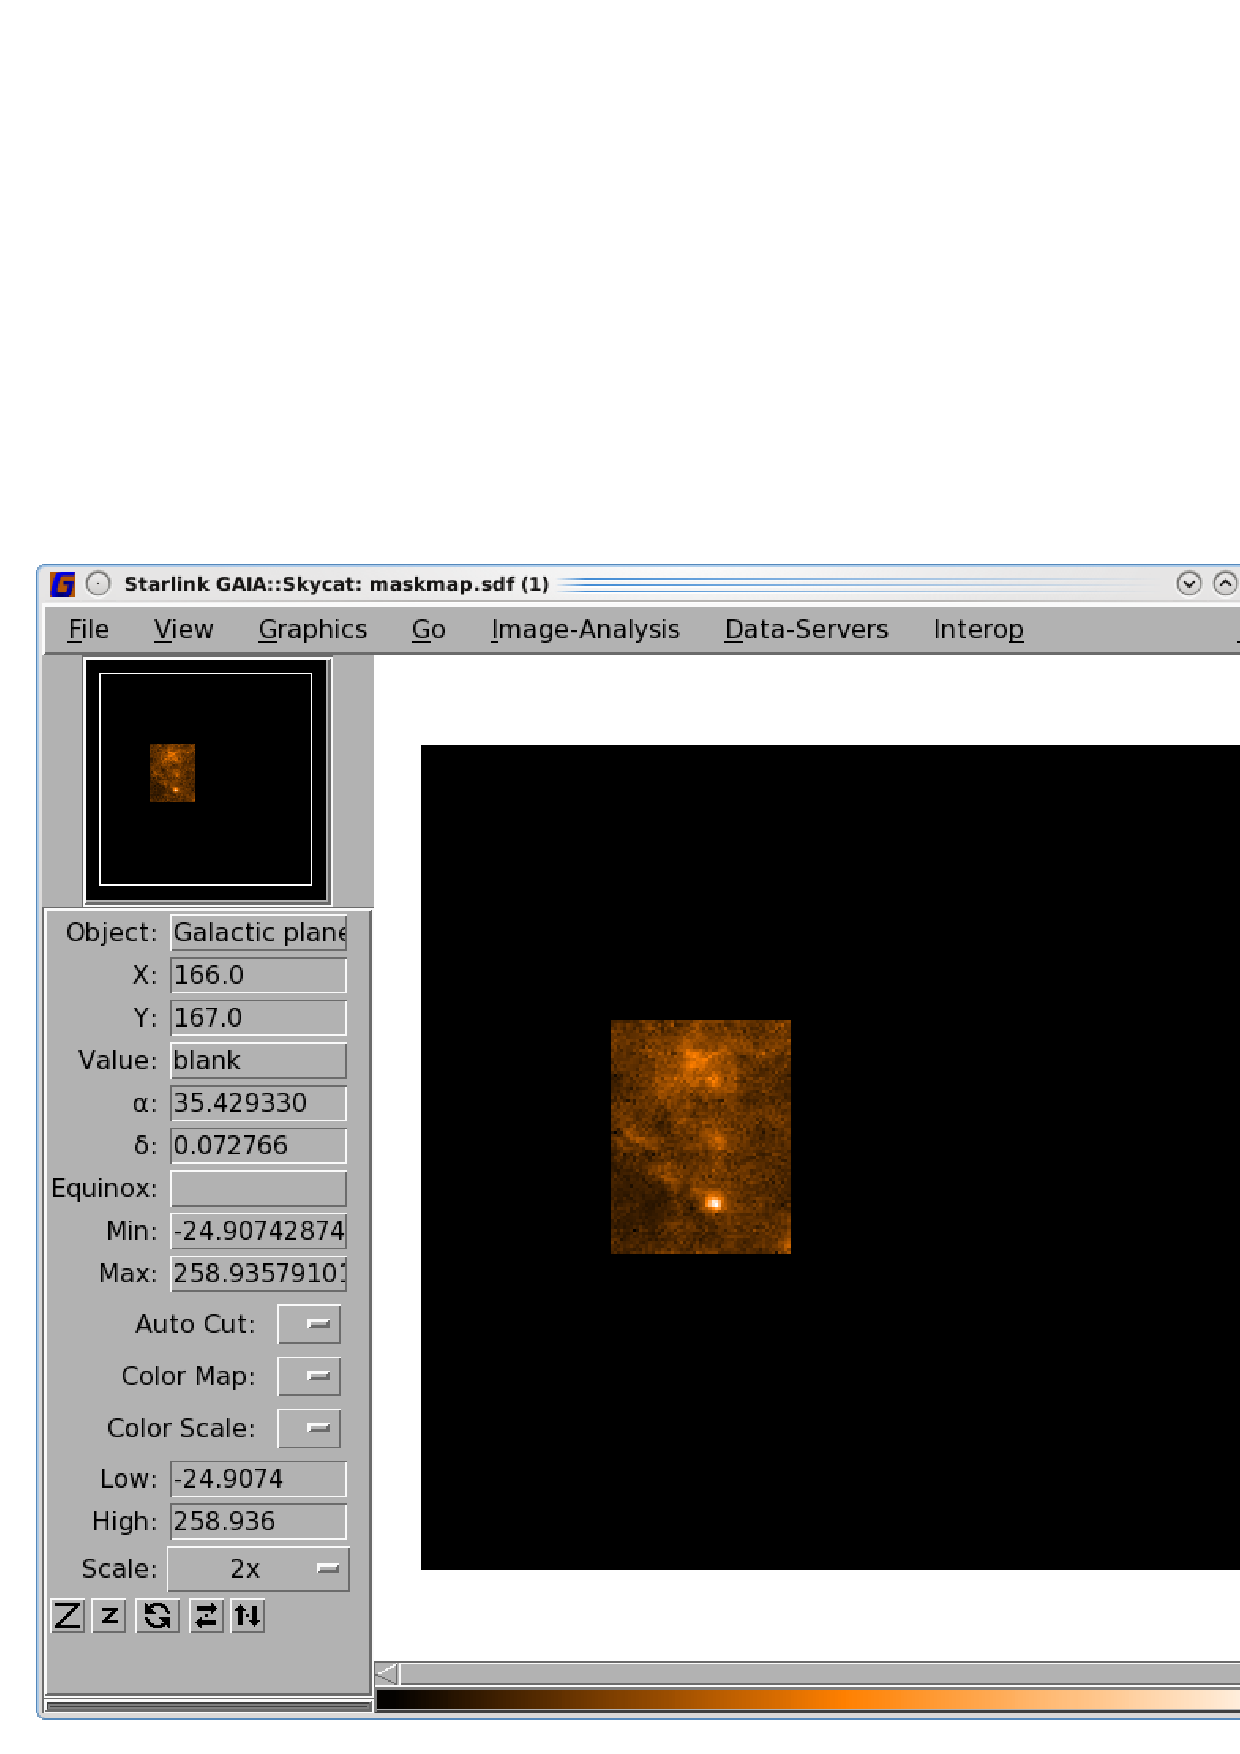
\includegraphics[height=7cm]{sc20_ard5}
\hspace{0.3cm}
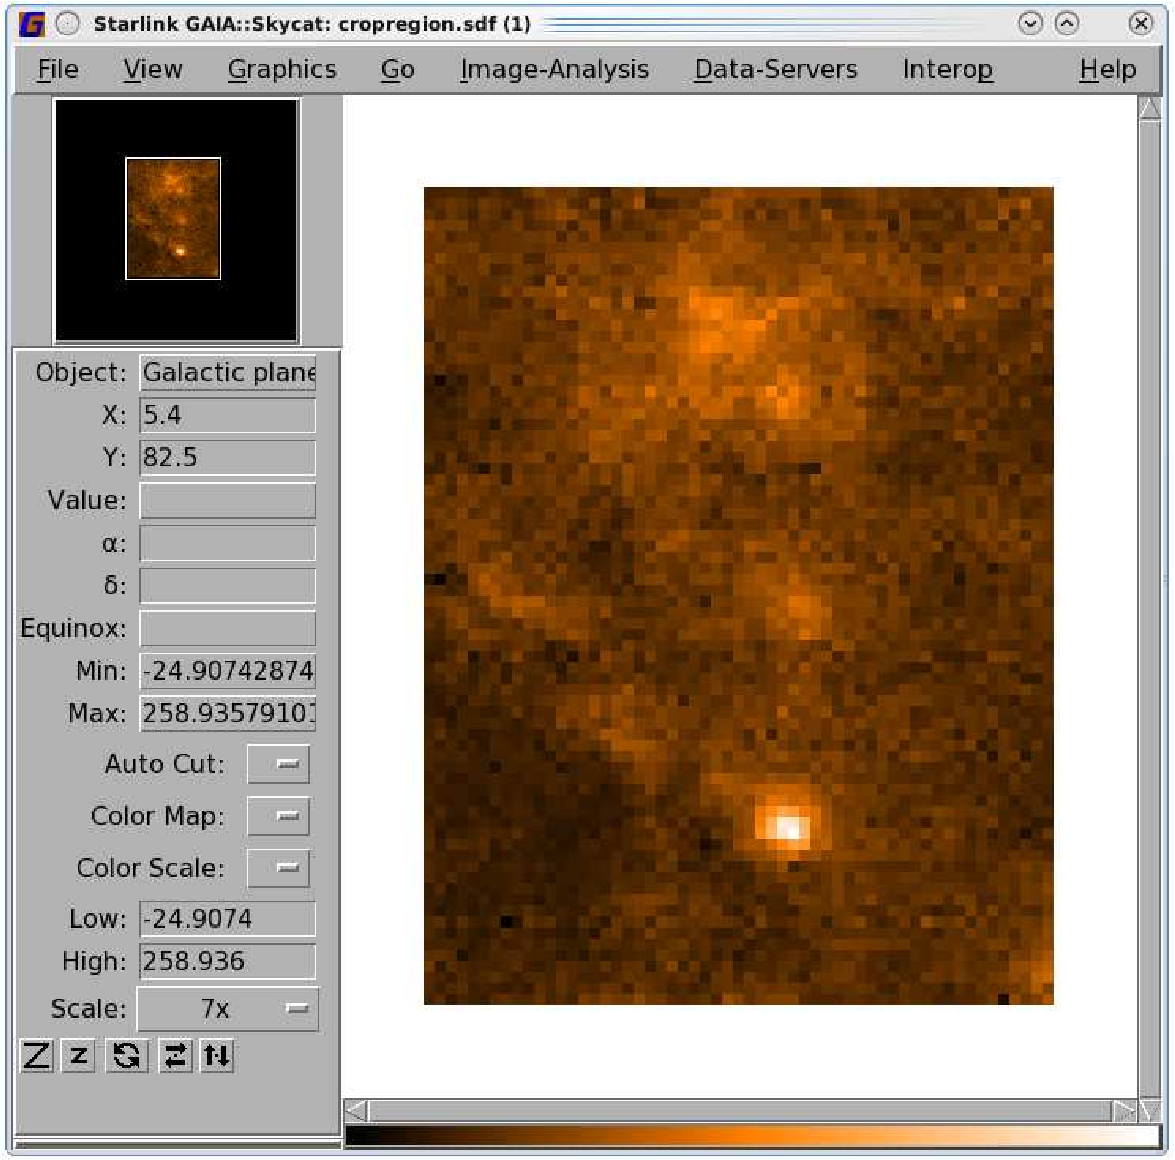
\includegraphics[height=7cm]{sc20_ard6}
\caption[Cropping a region of a two-dimensional map.]{\label{fig:crop}(Left) After
  applying the ARD mask, the cropped region is still surrounded by blank pixels.
  (Right) The blank pixels have been trimmed using \ndfcopy\ with the
  \param{trimbad} option.}
\label{fig:ardmask}
\end{center}
\end{figure}

\newpage
\section{\xlabel{holes}Filling holes in your map}
\label{sec:holes}

You may come across empty pixels in your map due to dead receptors or
receptors which have failed quality assurance in the pipeline. The
second half of 2013 in particular had only twelve working receptors for
HARP.

You can fill these holes using \Kappa:\fillbad. This replaces the bad
values with a smooth function derived from neighbouring values,
derived by iterating to a solution of Laplace's equation.

The default values for \fillbad\ will fill the holes but smooths by five
pixels along each axis. If you prefer not to smooth in the spectral
axis, set the parameter \param{size} to [$s$,$s$,0] where $s$ is the scale
length in pixels.  The zero means do not smooth along the third axis.

The scale length should have a value about half the size of the
largest region of bad data to be replaced.  Since the largest bad
regions apart from the cube peripheries are two pixels across, a size
of 1 is appropriate.
\begin{terminalv}
% fillbad in=holeymap out=filledmap size="[1,1,0]"
\end{terminalv}
\cref{Figure}{fig:fillholes}{The figure below} shows an initial map
with holes and the final filled map.

\begin{figure}[ht!]
\begin{center}
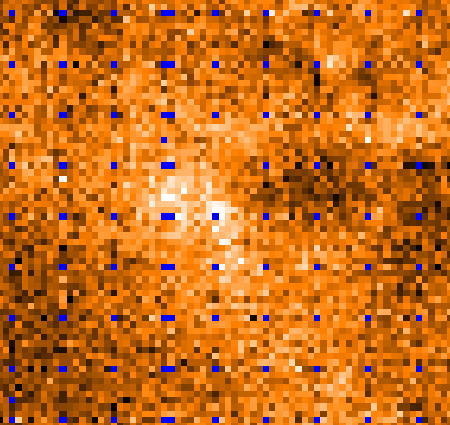
\includegraphics[width=0.48\linewidth]{sc20_holeyharp}
\typeout{sc20_holeyharp inserted on page \arabic{page}}
\hspace{0.5mm}
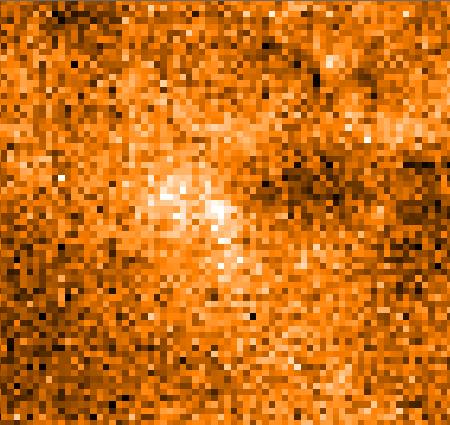
\includegraphics[width=0.48\linewidth]{sc20_polyfillaharp}
\typeout{sc20_polyfillaharp inserted on page \arabic{page}}
\caption[Filling holes in your HARP map with \fillbad.]{\label{fig:fillholes}
  Filling holes in your HARP map with \fillbad. Compare the original map
  (left) with the filled map (right).  A blue pixel indicates an
  undefined spectrum.}
\end{center}
\end{figure}


\section{\xlabel{noise}Checking the noise}
\label{sec:noise}

You can use \Kappa:\stats\ to check the noise in your map. It will
report the statistics for all pixels so be aware that noisy edges and
strong signal will contribute to the standard deviation. You can
mitigate this by trimming any noisy edges and by examining the square
root of the VARIANCE component (hereafter referred to as the error
component\footnote{No such component exists in the NDF.}) although
bright emission will still increase your noise. You can select the
error component with \param{comp=err} on the command line.
\begin{terminalv}
% stats file comp=err order
\end{terminalv}
Including the option \param{order} allows the ordered statistics such
as the median and percentiles to be reported. Note that percentile
options will need to be specified via the \param{percentiles}
parameter.

\begin{tip}
Remember the mean or median values will give you the noise when
using the error component.
\end{tip}

\subsection{Visualising the noise}

You can plot the noise or error component of your map using the
\textsc{Kappa} command \histogram. This allows you to visualise the
distribution with more ease. Again the \param{comp=err} option is
used.
\begin{terminalv}
% histogram mosaic comp=err range=! numbin=200
\end{terminalv}
The output is shown in \cref{Figure}{fig:noihisto}{the graphic below}.
An alternative to setting the number of bins via the \param{numbin}
parameter is to set the width of each bin using the \param{width}
parameter.

\begin{figure}[h!]
\begin{center}
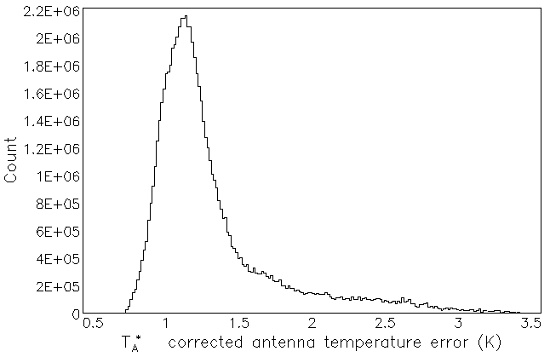
\includegraphics[width=0.6\linewidth]{sc20_noihisto1}
\typeout{sc20_noihisto1 inserted on page \arabic{page}}
\caption[
  A histogram of the error component.]{\label{fig:noihisto}
  The error component plotted with \histogram.}
\end{center}
\end{figure}

It is also useful to view the noise map itself.
\cref{Figure}{fig:noisemap}{The figure below} shows how to select the
error component in \gaia. Other options available from the
\guiwindow{Select NDF in container file} window include the exposure
time, the effective time and, if \param{spread=nearest} when running
\makecube, the system temperature. To return to your main image select
the top level and click the \guithing{Data} button.

\begin{tip}
TIP: You can write out the error component into a new file using
\ndfcopy.
\begin{terminalv}
% ndfcopy map comp=err noisemap
\end{terminalv}
\end{tip}


\begin{figure}[h!]
\begin{center}
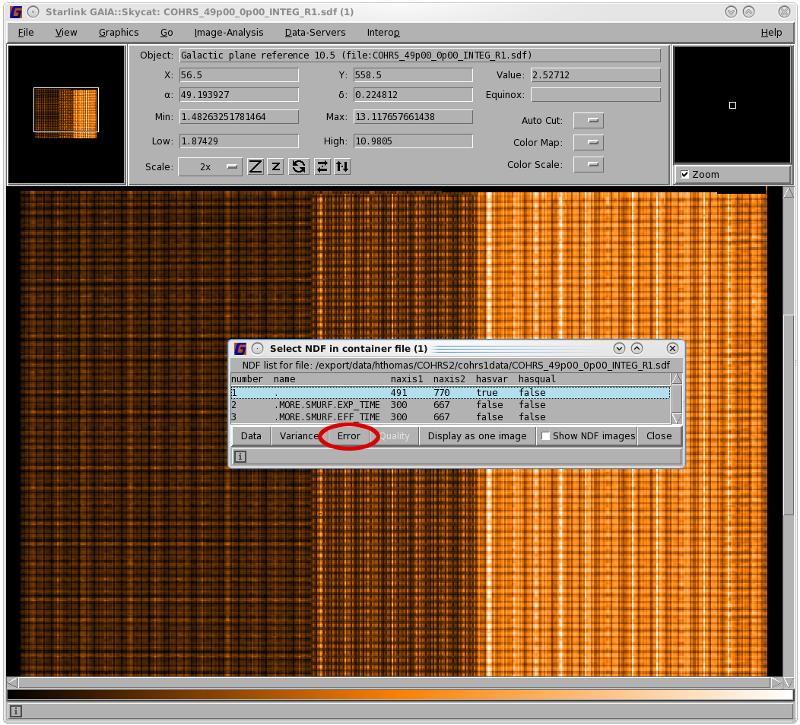
\includegraphics[width=0.6\linewidth]{sc20_noimap}
\typeout{sc20_noimap inserted on page \arabic{page}}
\caption[The noise map of a mosaic of tiles.]{\label{fig:noisemap}
  The noise map of a mosaic of tiles taken in differing weather
  conditions.}
\end{center}
\end{figure}


\subsection{HARP Flatfielding}
\label{sec:flatfield}

The individual detectors in the HARP array do not respond exactly the
same to the incoming signal, returning different temperatures for the
same flux.  If uncorrected, this can lead to artificial net-like
patterns in the reduced spectral cube.  As with any flatfield
correction, the goal is to expose to a uniform source to measure the
relative responses of the detectors.  However, this is not possible
with HARP observations, and the approach is assume that during an
observation the detectors see approximately the same signal from the
various sources.  For extended emission at low galactic latitudes this
is a reasonable assumption.  For isolated compact sources it is likely
to be invalid.

It may be possible to use a flatfield determined on the same night
in a high-signal region and apply that to a low-signal or
compact-source observation.  The flatfield can change during the
night, but it might better than no flatfield.

The method of Curtis et al. (2010)\cite{flat} creates a map for each detector
and integrates the measured flux in the main spectral line.  Use the
\param{DETECTORS} parameter to create a spectral cube from just that
detector.

\begin{terminalv}
% makecube in=rawfile out=cube_H01 detectors="'H01'" autogrid
\end{terminalv}

The simplest way to sum the flux across a line run \stats\ over a chosen
spectral range, such as $-5$\kms\ to 7.2\kms.

\begin{terminalv}
% stats cube_H01"(,,-5.0:7.2)"
\end{terminalv}

If there might be bad pixels present, the mean is more accurate than the sum.
This assumes that the line is located within these bounds across the whole
spatial region.  It is wise not to push too far into the wings of the line and
baseline errors and noise have a greater impact on the integrated flux.

The receptors are normalised to the flux of the reference receptor,
near the centre, normally H05, but given by the FITS header \param{REFRECEP}.


There are other methods in \ORACDR, one to cope with multiple lines.
It sums all the signal above some threshold, such as the median plus four
standard deviations, to exclude the baseline noise.  Since the flat
ratio biases this sum, \ORACDR\ iterates to converge to a solution.

\clearpage
\chapter{\xlabel{advanced}Advanced Analysis}
\label{sec:advanced}

\section{\xlabel{coords}Changing co-ordinate frames}

Co-ordinate systems of regridded Starlink files are described by the
world co-ordinate system, (WCS). There are a number of basic co-ordinate
systems (or frames) common to all NDFs; these are described by their
DOMAIN (essentially their name) and are PIXEL, AXIS, GRID and
FRACTION. Additional frames can be stored in the WCS component. Two
common additional frames are SKY and SPECTRUM. SKY refers to
two-dimensional frames (known as SkyFrames) which describe sky
co-ordinates. SPECTRUM refers to one-dimensional frames (known as
SpecFrames) that describe a position within a spectrum.

The choice of co-ordinates within the SkyFrame or SpecFrame is called
the system. For example, for SkyFrames this may be Galactic or FK5,
while for SpecFrames this may be velocity or frequency.

The current frame and the system can both be changed using the \Kappa\
applications \wcsframe\ and \wcsattrib. The current frame for data
processed with \makecube\ (either manually or by the pipeline)
typically has a DOMAIN of SKY-DSBSPECTRUM. The compound name refers to
the first two axes of the frame having sky co-ordinates and the third
axis having dual side-band spectral units. You can check this with
\ndftrace:

\begin{terminalv}
% ndftrace file | grep Domain
\end{terminalv}
You can change the attributes of a cube using \wcsattrib. To change
the SkyFrame co-ordinate system set the \att{System} attribute.
\begin{terminalv}
% wcsattrib file set system galactic
\end{terminalv}
To change between velocity and frequency you also use the
\att{System} attribute. For SKY-DSBSPECTRUM the software knows which
axis is being referred to based on the option you supply (the third in
this case).
\begin{terminalv}
% wcsattrib file set system freq
% wcsattrib file set system vrad
\end{terminalv}
Once a cube has been collapsed and is two-dimensional its Frame
becomes SKY. If you need to change frames manually use \wcsframe.
\begin{terminalv}
% wcsframe file sky
\end{terminalv}

For offset co-ordinates you will need to set the system
\param{skyrefis} to origin. The final two lines in the example below
convert the offset units to arcseconds instead of radians.
\begin{terminalv}
% wcsattrib file set skyrefis origin
% wcsattrib file set 'format(1)' 's.*'
% wcsattrib file set 'format(2)' 's.*'
\end{terminalv}

%
%\section{\xlabel{despike}Despiking}

%Interference spikes are sometimes found in ACSIS data. Spikes should
%be quite conspicuous in the data cube as they occur at the same
%frequency throughout the observed cube and at (almost) uniform
%intensity. It is probably best to eliminate spikes in your data cube
%from the raw time series, i.e. before running \makecube\ or any other
%processing on your data.
%
%If you suspect you have a spike in your
%data \cref{Appendix}{app:spike}{} describes the procedure for identifying
%the position of the spike and masking it out. %

\section{\xlabel{hybrid}Hybrid Data}

To merge two \htmlref{hybrid}{sec:hybrid}{} observations run \wcsalign\ on both files.
\begin{terminalv}
% wcsalign in="'rawfile_01.sdf,rawfile_02.sdf'" insitu lbnd=! ubnd=! ref=!
\end{terminalv}
Next trim each subsystem to remove noisy ends of the spectra in the
overlap region. You can get the pixel bounds from \ndftrace\ (here
1024). The example below trims 35 channels from the `left' of
rawfile\_01 and 24 channels from the `right' of rawfile\_02.
\begin{terminalv}
% ndfcopy in='rawfile_01(35:1024,,)' out=trimfile_01
% ndfcopy in='rawfile_02(0:1000,,)'  out=trimfile_02
\end{terminalv}

At this point the subsystems are aligned pixel for pixel.  So a
subtraction with \sub\ will generate the differences in the trimmed
overlap region analysed by \stats\ from which the median is found,
which is 0.04 in the example below.

\begin{terminalv}
% sub trimfile_01 trimfile_02 overlap_12
% stats overlap_12 order
% cadd trimfile_02 0.04 offsetfile_02
\end{terminalv}

You can then apply the offset to the second subsystem with \cadd.
Then the first subsystem can then be merged using \wcsmosaic.
\begin{terminalv}
% wcsmosaic in='"rawfile_01,offsetfile_02"' out=rawfile12 lbnd=! method=nearest accept
\end{terminalv}
You should check the final spectra to make sure there is no noise bump
in the middle where they overlap.

Another technique to locate the noisy edges is apply \collapse\ to all
the spectra in an observation using the \param{estimator=sigma}
option then smooth.  The composite formed will show a smooth noise profile,
increasing dramatically at its end.  The trim limits can be estimated
manually, or a linear trend fit with \mfittrend\ will return the bounds
of the flat low-noise portion of the spectrum in its \param{aranges}
parameter.

\begin{terminalv}
% collapse in=rawfile_01 out=profile axis=spec wlim=0.0 estimator=sigma trim
% block in=profile out=profile_sm box=25
% mfittrend in=profile_sm out=junk axis=1 method=region auto order=0
% parget aranges mfittrend
\end{terminalv}

In the example above, \parget\ should return just one pair of pixel
co-ordinates, which can then form part of an NDF section to extract the
non-noisy part of rawfile\_01 using \ndfcopy. If there is more than one
range you want to use the lowest and highest values.

\section{\xlabel{pv}Position-velocity diagram}

You can create a position-velocity map by collapsing over the skylat
or skylon axis of a reduced cube. Use the \Kappa\ command \collapse\ with
\param{axis=skylat}:

\begin{terminalv}
collapse in=reduced.sdf axis=skylat estimator=sum out=pv
\end{terminalv}
You can view your pv map with  \gaia\ or \display.

To obtain a position-velocity map at an arbitrary angle, there is a
\xref{\textsc{pvslice}}{sun237}{pvslice} in the \datacube\ package.
This can be invoked directly, or its recipe extracted from the
\textsc{pvslice} script, if you know the co-ordinates of the ends of
the slice and do not need the graphics.

\section{\xlabel{channel}Creating channel maps}
\label{sec:channel}

The \Kappa\ application \chanmap\ creates a two-dimensional channel
map from a cube. It collapses along the nominated axis (with many of
the same parameters as \collapse). The number of channels to create is
given by \param{nchan} and these are divided evenly between your
ranges. The arrangement of the resulting panels is determined by the
shape parameter. The collapsed slices are tiled with no margins to
form the final image.

\begin{terminalv}
% chanmap in=cube axis=3 low=-10 high=5 nchan=6 shape=3 estimator=mean
\end{terminalv}
This grid of channel maps is filled from left to right, and bottom to
top. It can be viewed with \gaia\ (see \cref{Figure}{fig:chanmap}{}) or
with \display.
\begin{terminalv}
% display chanmap mode=faint noaxes lut=$STARLINK_DIR/bin/kappa/smooth3_lut
\end{terminalv}

Channel maps can also be created using \gaia. See
\cref{Section}{sec:gaiachannel}{Channel maps} for instructions.


\begin{figure}[h!]
\begin{center}
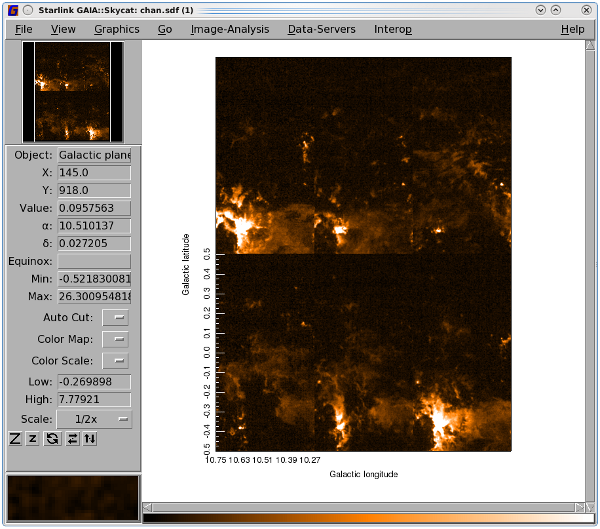
\includegraphics[width=0.8\linewidth]{sc20_chanmap}
\typeout{sc20_chanmap inserted on page \arabic{page}}
\caption[Displaying a channel map with \gaia.]{\label{fig:chanmap}
  Displaying a channel map with \gaia.}
\end{center}
\end{figure}

\section{\xlabel{clumpfinding}Clump finding}
\label{sec:clumpfind}

The \cupid\ application \findclumps\ can be used to generate a clump
catalogue. It identifies clumps of emission in one-, two- or
three-dimensional NDFs. You can select from the clump-finding
algorithms FellWalker, GaussClumps, ClumpFind or Reinhold. You must
supply a configuration file which lists the options for whichever
algorithm you chose (see the \xref{\textsc{cupid} manual}{sun255}{}
for a full list). The result is returned as a catalogue in a text file
and as a NDF pixel mask showing the clump boundaries (see
\cref{Figure}{fig:clumps2}{}). See
\cref{Appendix}{app:clumpfind}{Clump-finding Algorithms} for
descriptions of the various algorithms.

\begin{terminalv}
% findclumps in=map out=clumpmap outcat=clumps.FIT logfile=clumps.log \
  config=^myconfig.dat method=clumpfind rms=0.2 shape=polygon
\end{terminalv}

The shape option allows \findclumps\ to create a shape that should be
used to describe the spatial coverage of each clump in the output
catalogue. It can be set to " None", " Polygon" or " Ellipse". The shape
- as described in the output catalogue---is in "STC-S" format. STC-S is
a textual format developed by the IVOA for describing regions within
a WCS---\htmladdnormallink{see here for
details.}{http://www.ivoa.net/Documents/latest/STC-S.html}.
The STC-S descriptions are added as extra columns to the output catalogue.
\vspace{0.7cm}
\begin{figure}[h!]
\begin{center}
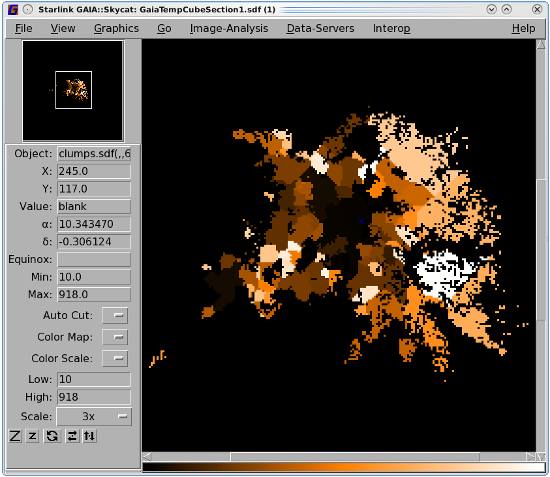
\includegraphics[width=0.7\linewidth]{sc20_clumps}
\typeout{sc20_clumps inserted on page \arabic{page}}
\caption[A velocity slice of the result of three-dimensional clump finding
viewed with \gaia.]{\label{fig:clumps2}
  A velocity slice of the result of three-dimensional clump finding viewed
  with \gaia. This output NDF contains boundaries of the clumps, with the
  value reflecting the number of pixels contained within that clump.}
\end{center}
\end{figure}

\begin{aligndesc}
\item[\textbf{Polygon}]
Each polygon will have, at most, 15 vertices. For two-dimensional data
the polygon is a fit to the clump's outer boundary (the region
containing all good data values). For three-dimensional data the
spatial footprint of each clump is determined by rejecting the least
significant 10\% of spatial pixels, where ``significance'' is measured
by the number of spectral channels that contribute to the spatial
pixel. The polygon is then a fit to the outer boundary of the
remaining spatial pixels.
\vspace{0.7cm}\\
\item[\textbf{Ellipse}]
All data values in the clump are projected onto the spatial plane and
``size'' of the collapsed clump at four different position angles---all
separated by 45$^\circ$---is found. The ellipse that generates
the same sizes at the four position angles is then found and used as
the clump shape.
\end{aligndesc}

You can plot the clump outlines over an image using \gaia. See Section
\ref{sec:plotclumps} for instructions.



\section{\xlabel{telluricsplat}Using SPLAT to identify telluric emission}
\label{sec:telluricsplat}

Occasionally you may see unexpected emission within your data. An
example is shown in \cref{Figure}{fig:telluric1}{}. In this figure, we
use the average spectrum feature (see
\cref{Section}{sec:gaiaaverage}{Displaying average spectrum with
GAIA}---and in this example---we see expected bright emission around
7\kms. In addition to the expected bright emission, we see some faint
emission around $-$30\kms.

\begin{figure}[h!]
\begin{center}
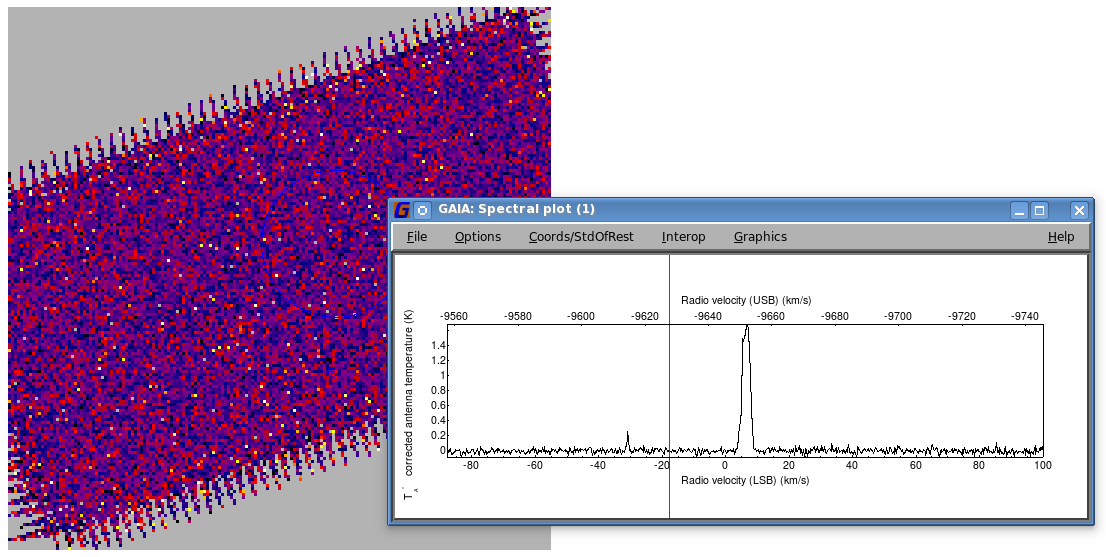
\includegraphics[width=0.7\linewidth]{sc20_splat_spectrum_example_telluric1.png}
\typeout{sc20_splat_spectrum_example_telluric1 inserted on page \arabic{page}}
\caption[An example of unexpected emission seen in \gaia.]{\label{fig:telluric1}
  An example of a spectrum with bright expected emission around 7\kms\ and
  unexpected emission around $-$30\kms. The data are displayed using \gaia.}
\end{center}
\end{figure}

We can use \splat\ to investigate this emission further (see
\cref{Section}{sec:gaiatosplat}{Sending spectra to SPLAT} on how to
open up a spectrum in \splat).

\begin{figure}[h!]
\begin{center}
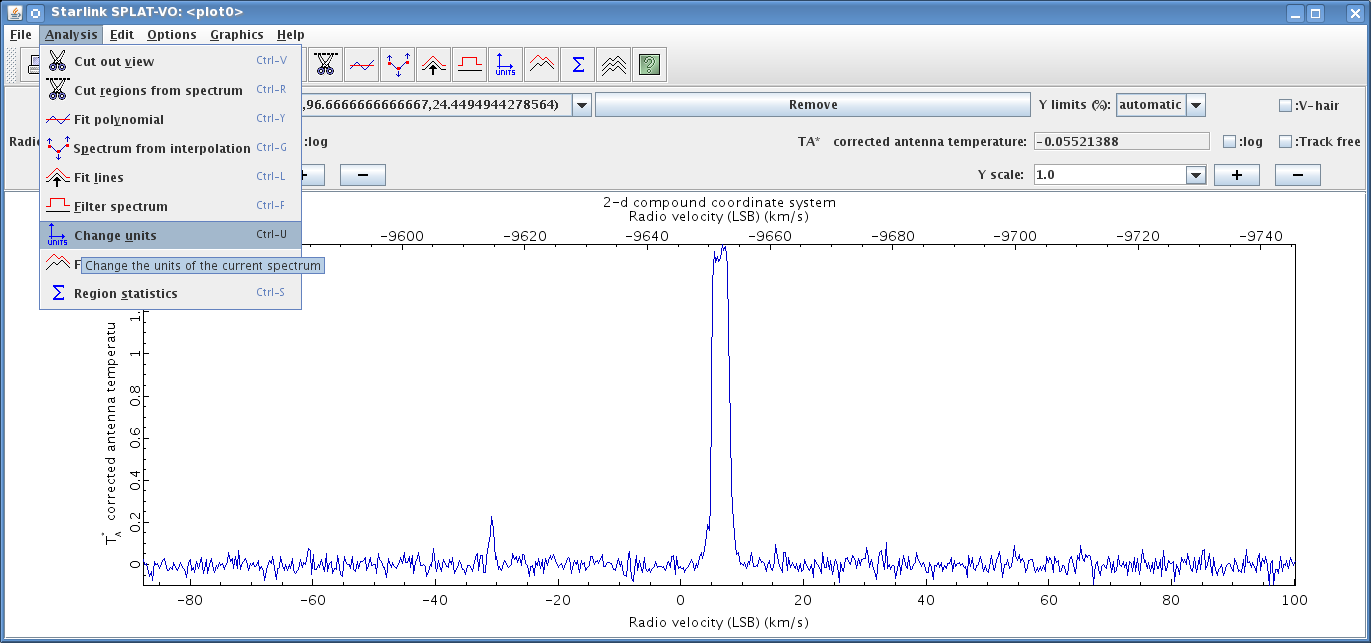
\includegraphics[width=0.7\linewidth]{sc20_splat_spectrum_example_telluric2.png}
\typeout{sc20_splat_spectrum_example_telluric2 inserted on page \arabic{page}}
\caption[blah]{\label{fig:telluric2}
  Displaying a channel map with \splat.}
\end{center}
\end{figure}

It is possible to use \splat\ to change the units to \guithing{Standard of rest: Observer}
by first going to \guithing{Analysis} and clicking on \guithing{Change units}.

\begin{figure}[h!]
\begin{center}
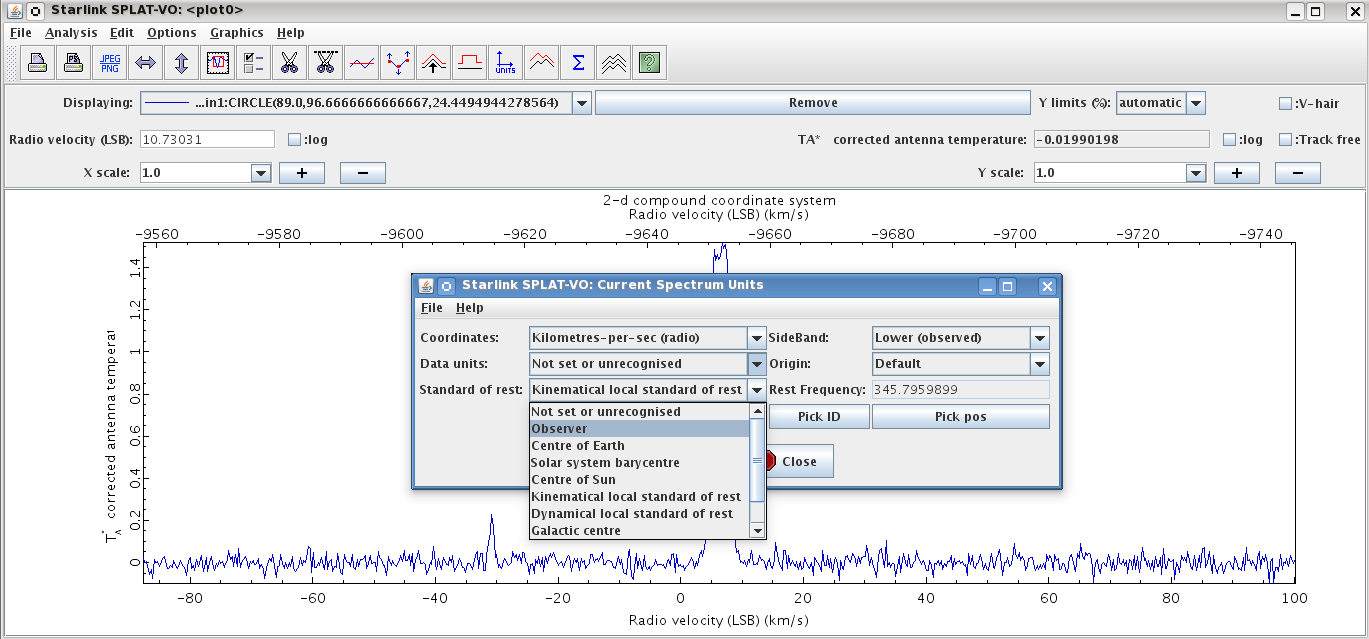
\includegraphics[width=0.7\linewidth]{sc20_splat_spectrum_example_telluric3.png}
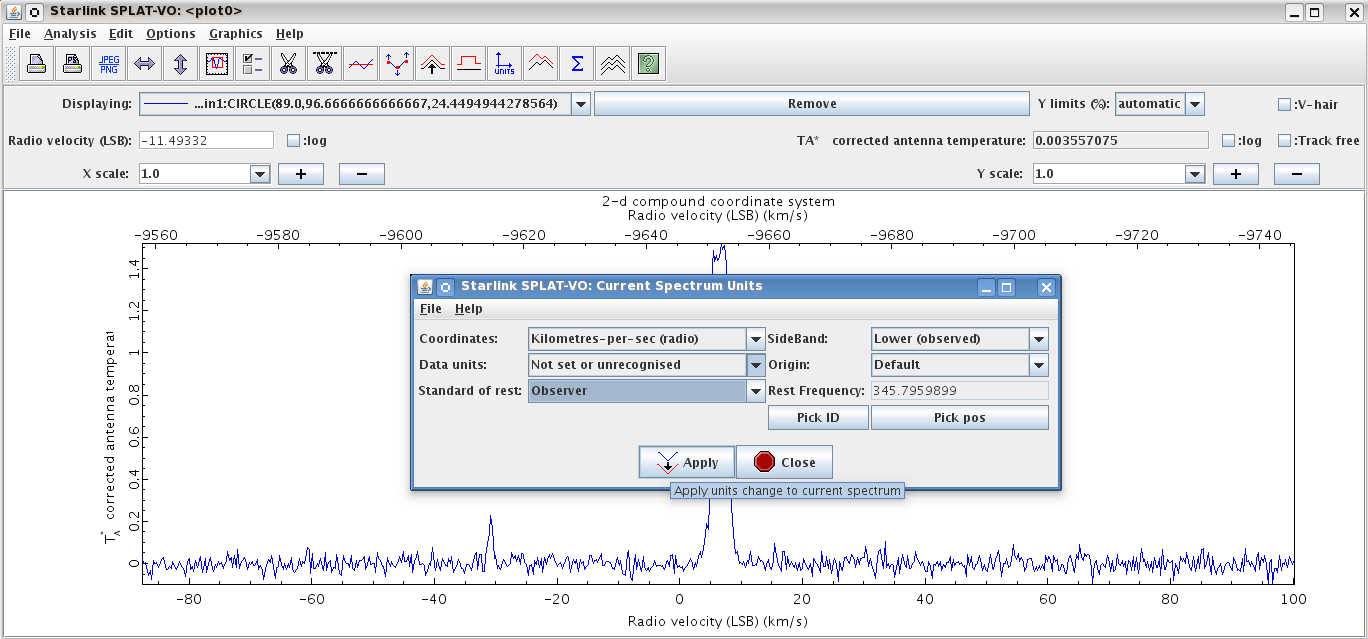
\includegraphics[width=0.7\linewidth]{sc20_splat_spectrum_example_telluric4.png}
\typeout{sc20_splat_spectrum_example_telluric3 and 4 inserted on page \arabic{page}}
\caption[blah]{\label{fig:telluric3}
  Select \guithing{Observer} from the \guithing{Standard of rest} Menu and select
\guithing{Apply}.}
\end{center}
\end{figure}

We then use the drop-down menu next to \guithing{Standard of rest} to select
\guithing{Observer} from the list, and select \guithing{Apply}.


\begin{figure}[h!]
\begin{center}
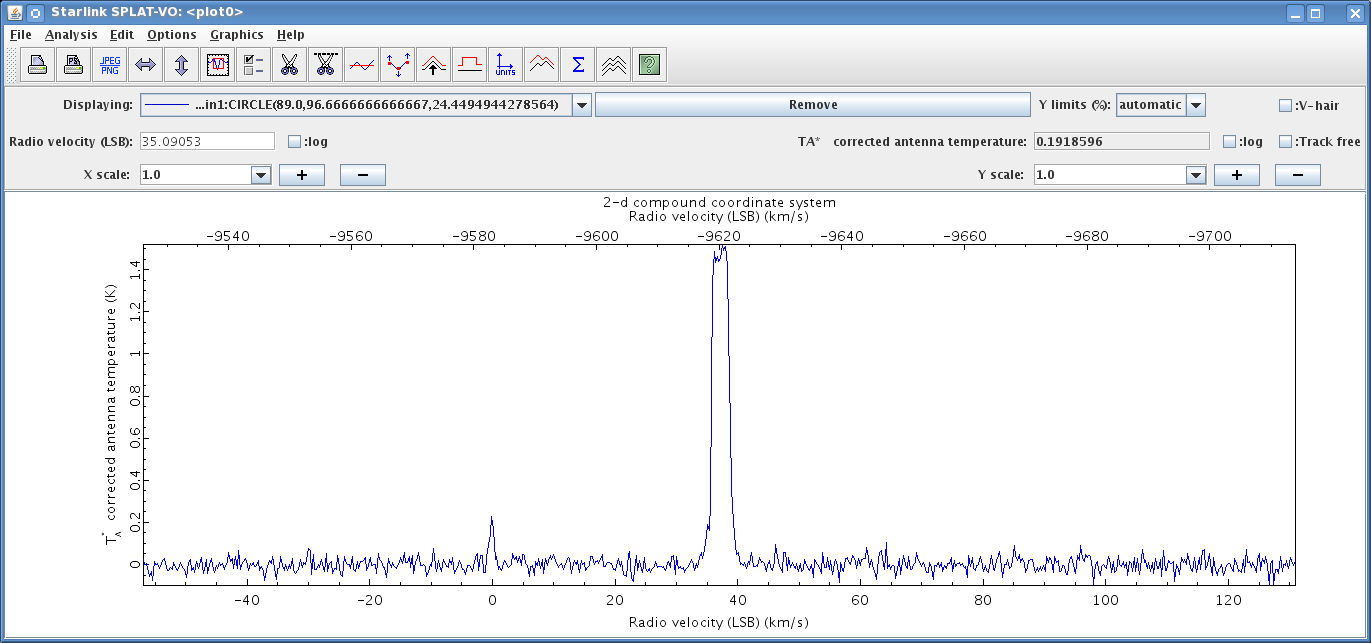
\includegraphics[width=0.7\linewidth]{sc20_splat_spectrum_example_telluric5.png}
\typeout{sc20_splat_spectrum_example_telluric5 inserted on page \arabic{page}}
\caption[blah]{\label{fig:telluric4}
  Spectrum from the observer rest frame. We see the unexpected line is
  found at 0\kms, and is likely telluric contamination.}
\end{center}
\end{figure}

Now we see the unexpected line is at 0\kms, and is therefore likely to be
contamination from telluric lines.

\clearpage
\chapter{\xlabel{gaia}Using GAIA}
\label{sec:gaia}

\section{Removing a baseline with GAIA}
\label{sec:gaiabaseline}

\begin{enumerate}[label=(\textbf{\arabic*})]
\item Select the spectrum you want to use as your template for the entire cube.

\item Select the Baseline tab in the \guiwindow{Display image sections
of a cube} window.

\item Select the order of the baseline you want to fit and remove.

\item Check the \guithing{Show limits on plot} button to
interactively draw your baseline windows. You can click and drag the
edges of these limit lines in the \guiwindow{Spectral plot} window.

\item Check \guithing{Enable} for each new baseline window you want to define.

\item Click \guithing{Run}.
\end{enumerate}

\begin{figure}[h!]
\begin{center}
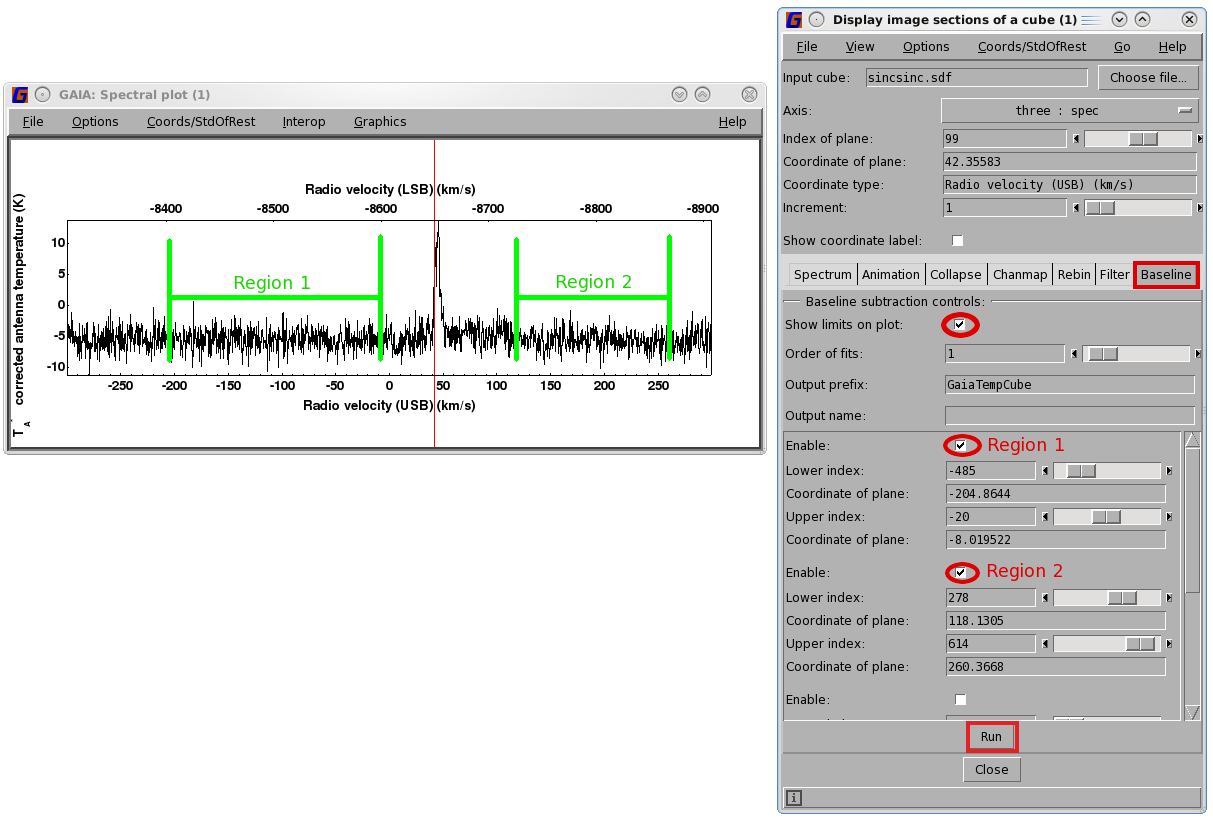
\includegraphics[width=0.9\linewidth]{sc20_gaia_baseline}
\typeout{sc20_gaia_baseline inserted on page \arabic{page}}
\caption[Removing a baseline with \gaia.]{\label{fig:gaiabaseline}
  Removing a baseline with \gaia.}
\end{center}
\end{figure}

\section{Creating channel maps with GAIA}
\label{sec:gaiachannel}

You can display channel maps in \gaia\ by selecting the region of a
spectrum you wish to collapse over. You can use a spectrum from any of
the pixels in the cube and the region selected will be applied to the
whole map.

\begin{enumerate}[label=(\textbf{\arabic*})]
\item  Select the spectrum you want to use as your template for the entire cube.

\item Select the \guithing{Chanmap} tab in the \guiwindow{Display
image sections of a cube} window.

\item Check the \guithing{Show limits on plot} box to interactively
draw the range over which to collapse your cube. You can click and
drag the end-bars of the limit lines in the \guiwindow{Spectral plot}
window.

\item Select the collapse method (Max is chosen in the example).

\begin{figure}[h!]
\begin{center}
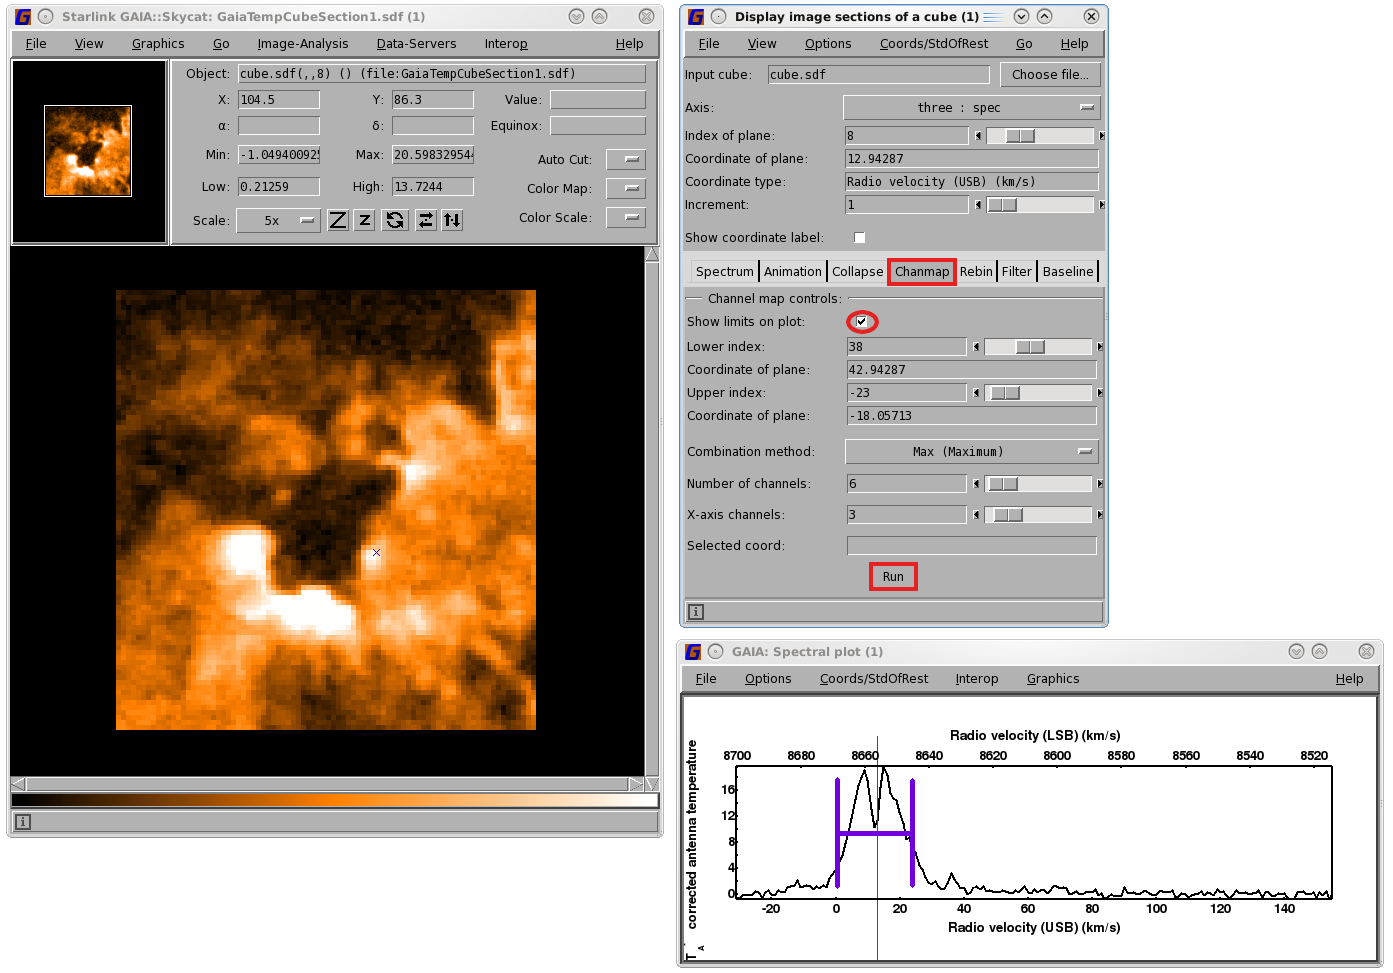
\includegraphics[width=0.93\linewidth]{sc20_gaia_channel1}
\typeout{sc20_gaia_channel1 inserted on page \arabic{page}}
\caption[Creating a channel map with \gaia.]{\label{fig:gaia_chan1}
  Creating a channel map with \gaia.}
\end{center}
\end{figure}

\item Use the slider bars to select the total number of channels you
want to generate and the number of \textit{x}-axis channels. The
\textit{x}-axis channel number sets the aspect ratio for the resulting
display grid.

\item Click \guithing{Run}. The result is shown in the figure below.

\begin{figure}[t!]
\begin{center}
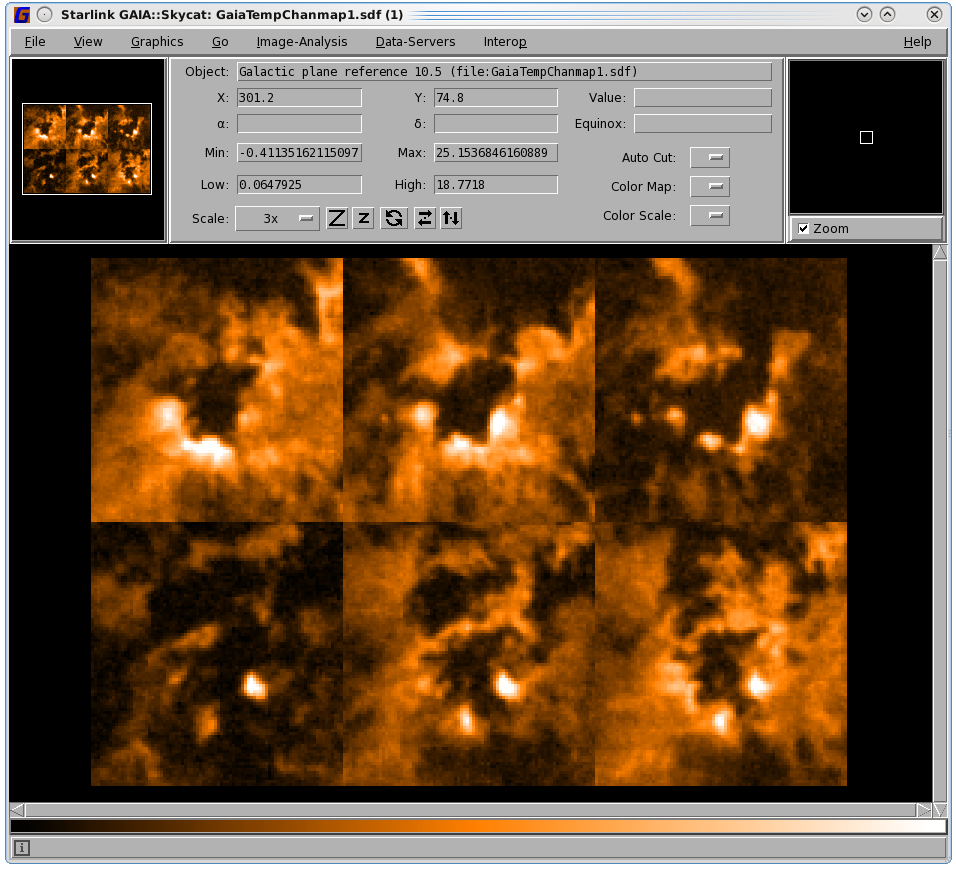
\includegraphics[width=0.6\linewidth]{sc20_gaia_channel2}
\typeout{sc20_gaia_channel2 inserted on page \arabic{page}}
\caption[Channel map created with \gaia.]{\label{fig:gaia_chan2}
  Channel map created with \gaia.}
\end{center}
\end{figure}
\end{enumerate}


\section{Contouring with GAIA}
\begin{enumerate}[label=(\textbf{\arabic*})]
\item  Open the map you wish to contour over.

\item Select \guithing{Image-Analysis$>$Contouring} from the menu bar
across the top of the main window.

\item Select the file you wish to contour in the \guiwindow{Contouring} window.

\item Generate your contours in the \guithing{Generate} tab found on
the left-hand side of the \guiwindow{Contouring} window. The example
below defines linearly spaced contours starting at 900K. Clicking the
\guithing{Generate} button will return you to the Levels tab.

\begin{figure}[h!]
\begin{center}
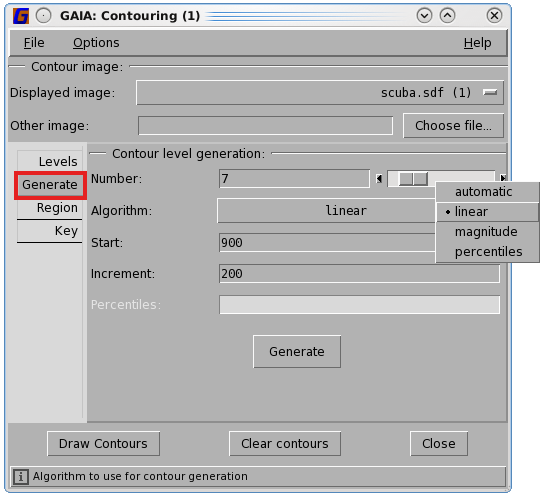
\includegraphics[width=0.4\linewidth]{sc20_contouring1}
\typeout{sc20_contouring1 inserted on page \arabic{page}}
\caption[Setting contours with \gaia.]{\label{fig:gaia_contour1}
  Setting contours with \gaia.}
\end{center}
\end{figure}

You can also input or edit the contour levels manually in the \guithing{Levels} tab.

\item Customise the look of your contours under the
\guithing{Options} menu. You can experiment with the other tabs
(Region and Key) for options concerning contour area and legend.

\begin{figure}[h!]
\begin{center}
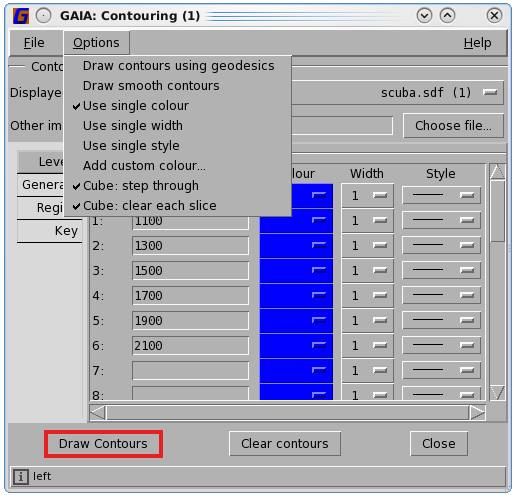
\includegraphics[width=0.4\linewidth]{sc20_contouring2}
\typeout{sc20_contouring2 inserted on page \arabic{page}}
\caption[Formatting contours with \gaia.]{\label{fig:gaia_contour2}
  Formatting contours with \gaia.}
\end{center}
\end{figure}

\item Click the \guithing{Draw Contours} button to make the contours
appear over your map in the main window. If you are contouring over a
cube you can scroll through the velocity axis whilst the contours
remain fixed on top.

\begin{figure}[h!]
\begin{center}
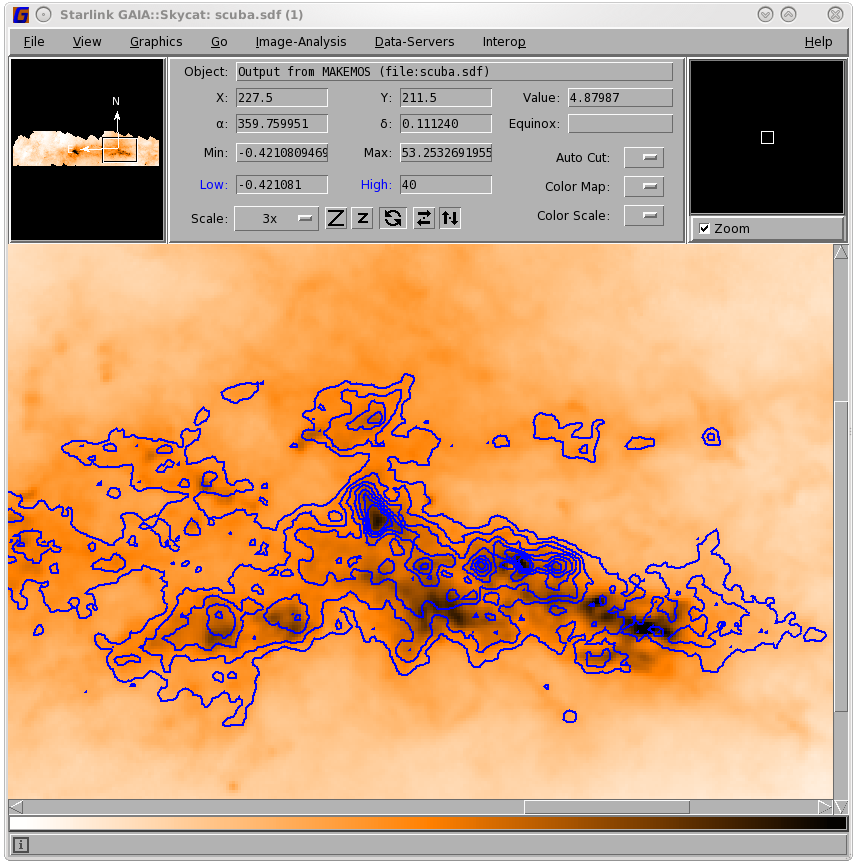
\includegraphics[width=0.6\linewidth]{sc20_contouring6}
\typeout{sc20_contouring6 inserted on page \arabic{page}}
\caption[Contoured map in \gaia.]{\label{fig:gaia_contour3}
  Contoured map in \gaia.}
\end{center}
\end{figure}

\item To add a second set of contours select \guithing{File$>$New
window} in the top menu of the \guiwindow{Contouring} window. Here you
can define a second image to be contoured and specify new levels and
appearance. Open as many new contouring windows as necessary.

To save the graphic, there is a \guithing{File} $>$ \guithing{Print},
but some people prefer a tool with a capture facility such as
\textsc{xv}.

\end{enumerate}

\section{Overlaying clumps and catalogues with GAIA}
\label{sec:plotclumps}

\gaia\ can display two- or three-dimensional clump catalogues that
have been generated by the \cupid\ routine \findclumps\ (see
\cref{Section}{sec:clumpfind}{Identifying Clumps}). Clump catalogues
in this format are also available for download from the JCMT Science
Archive.

\begin{enumerate}[label=(\textbf{\arabic*})]
\item Open your cube for three-dimensional clump finding or your
integrated map for two-dimensional clump finding.

\item Select \guithing{Image-Analysis$>$Positions$>$Import CUPID
catalogue} from the menu bar across the top of the main window. Note
that for two-dimensional catalogues an alternative route is to select
\guithing{Data-Servers$>$Local catalogs}. In this case you can skip
Step 3.

\begin{figure}[h!]
\begin{center}
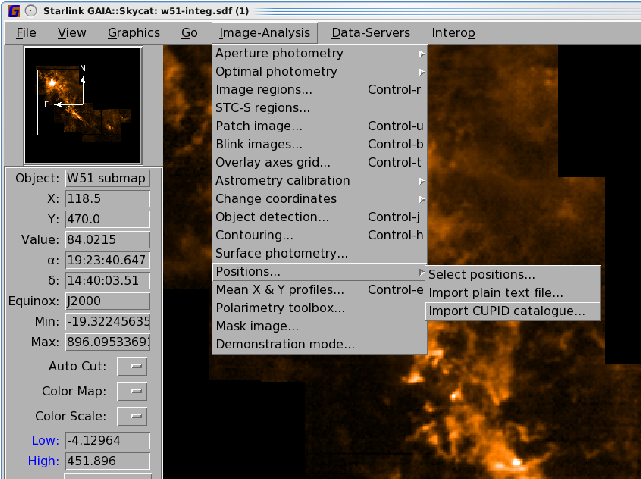
\includegraphics[width=0.5\linewidth]{sc20_plotclumps2b}
\typeout{sc20_plotclumps2b inserted on page \arabic{page}}
\caption[Importing a \cupid\ catalogue with \gaia.]{\label{fig:gaia_clumps1}
  Importing a \cupid\ catalogue with \gaia.}
\end{center}
\end{figure}

\begin{figure}[h!]
\begin{center}
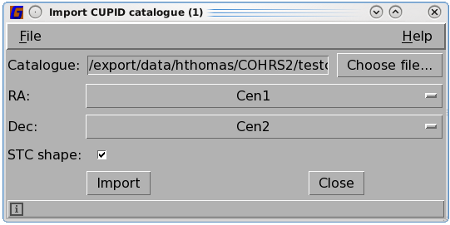
\includegraphics[width=0.5\linewidth]{sc20_plotclumps3}
\typeout{sc20_plotclumps3 inserted on page \arabic{page}}
\caption[Catalogue window in \gaia.]{\label{fig:gaia_clumps2}
  Catalogue window in \gaia.}
\end{center}
\end{figure}

\item In the \guiwindow{Import CUPID catalogue} window, select a file
with the \guithing{Choose file}... button. For polygon shapes tick
the STC shape box. You can change the RA/Dec co-ordinates from
Cen1/Cen2, which give the central position of the clumps, to
Peak1/Peak2 which give the position of the peak within them.

\item A catalogue window for your FITS file will appear listing all
the sources and their positions and extents.

\begin{figure}[h!]
\begin{center}
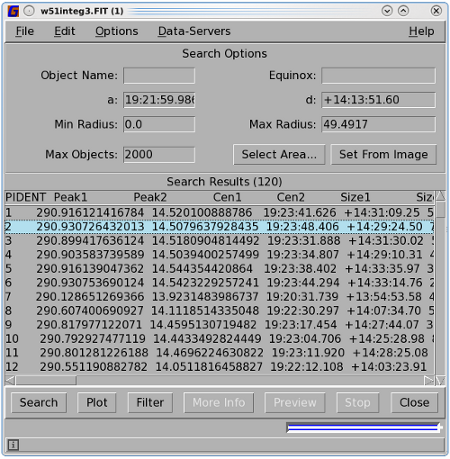
\includegraphics[width=0.5\linewidth]{sc20_plotclumps5}
\typeout{sc20_plotclumps5 inserted on page \arabic{page}}
\caption[Catalogue window in \gaia.]{\label{fig:gaia_clumps3}
  Catalogue window in \gaia.}
\end{center}
\end{figure}

\item Outlines of your clumps, or symbols at the peak positions, will
be automatically overlaid on your map. If this does not happen, click
the \guithing{Plot} button on the catalogue window. When you click on
a clump from the catalogue list the outline of that clump will appear
in bold on your map.

\begin{figure}[h!]
\begin{center}
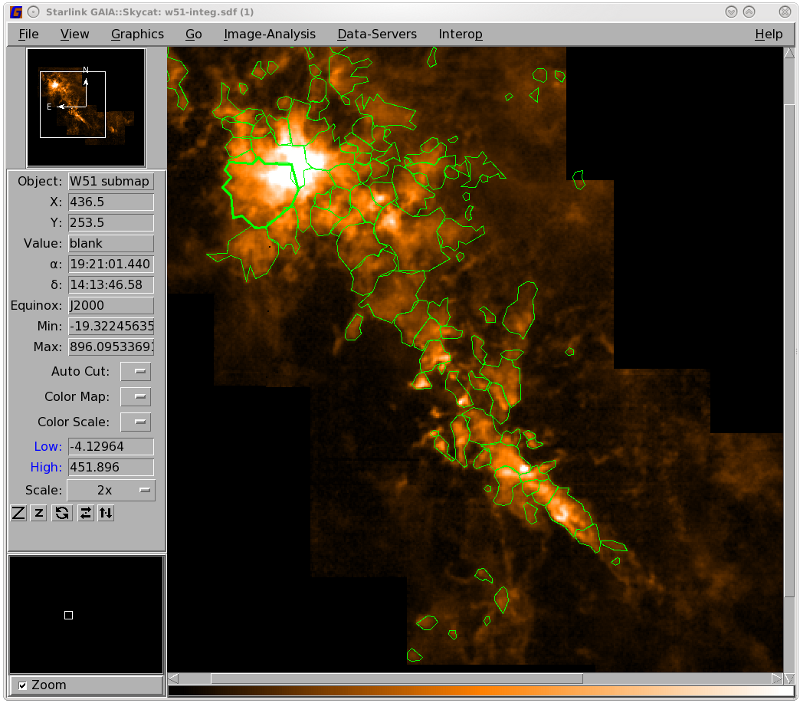
\includegraphics[width=0.6\linewidth]{sc20_plotclumps6}
\typeout{sc20_plotclumps6 inserted on page \arabic{page}}
\caption[Clumps outlined overlaid on integrated map in \gaia.]{\label{fig:gaia_clumps4}
  Clumps outlined overlaid on integrated map in \gaia.}
\end{center}
\end{figure}

\item If you are displaying a three-dimensional catalogue over a cube,
it will only display clumps which include data from the current slice.
The clumps shown will update as you move through the cube.

\end{enumerate}

\section{Displaying average spectrum with GAIA}
\label{sec:gaiaaverage}

\begin{enumerate}[label=(\textbf{\arabic*})]
\item Select the \guithing{Spectrum} tab in the \guiwindow{Display
image sections of a cube} window.

\item Define the shape of your region by selecting one of the
\guithing{Define region} buttons (a circle is chosen in the example
below).

\item Select the combination method (Mean is chosen in the example below).

\begin{figure}[h!]
\begin{center}
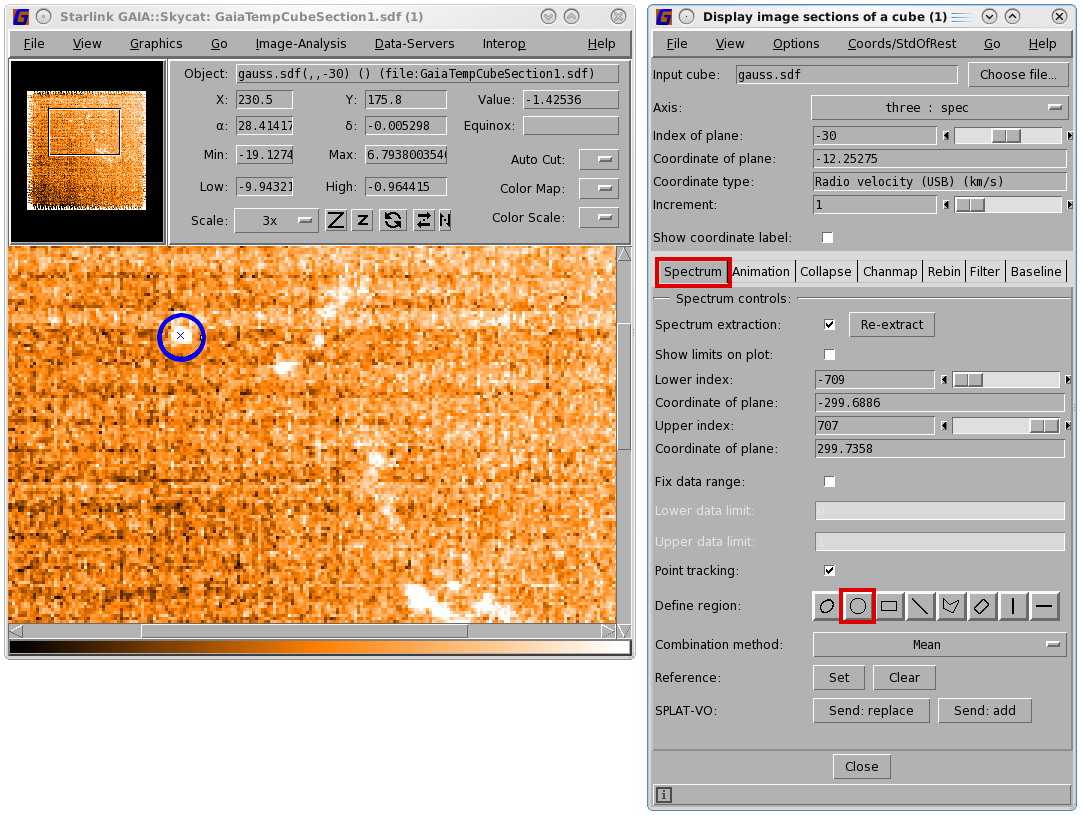
\includegraphics[width=0.8\linewidth]{sc20_gaia_avgspec1}
\typeout{sc20_gaia_avgspec1 inserted on page \arabic{page}}
\end{center}
\caption[Displaying an average spectrum with \gaia.]{\label{fig:gaia_avgspec1}
  Displaying an average spectrum with \gaia.}
\end{figure}

\item Draw the shape on your map by clicking and dragging the mouse.
The \guiwindow{Spectral plot} window will automatically update to show
your combined spectrum. You can re-position and resize your shape at
any time. You can see from \cref{Figure}{fig:gaia_avgspec2}{} that the
averaged spectrum gives a much clearer profile of the source.


\begin{figure}[ht!]
\begin{center}
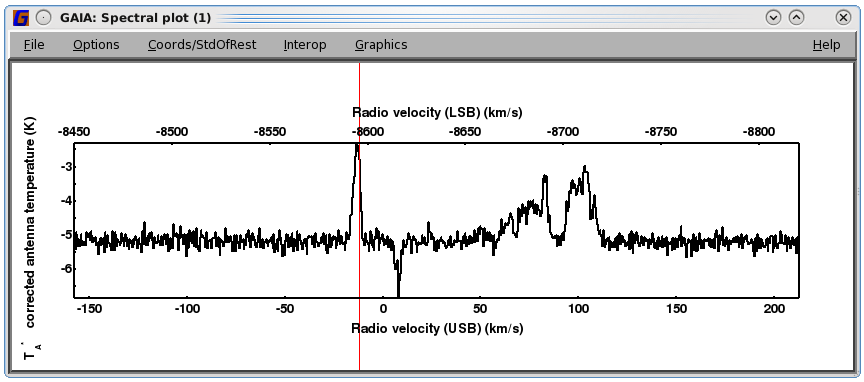
\includegraphics[width=0.48\linewidth]{sc20_gaia_avgspec2}
\typeout{sc20_gaia_avgspec2 inserted on page \arabic{page}}
\hspace{0.5mm}
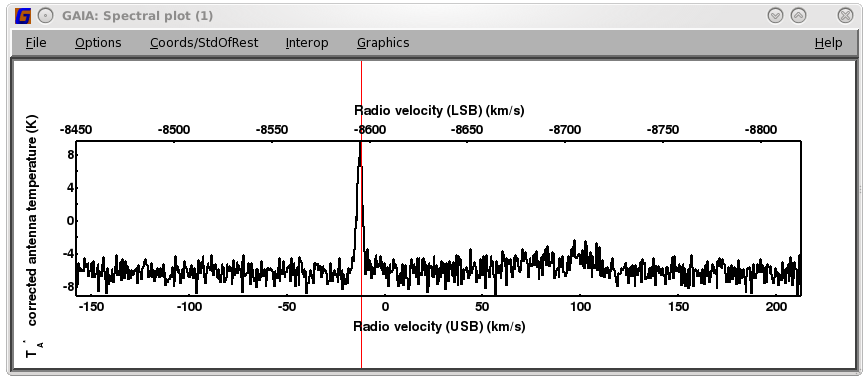
\includegraphics[width=0.48\linewidth]{sc20_gaia_avgspec3}
\typeout{sc20_gaia_avgspec3 inserted on page \arabic{page}}
\caption[Example of averaged spectra.]{\label{fig:gaia_avgspec2}
 (Left) Average of the spectra within the blue circle in the figure
  above. (Right) Single spectrum from the centre of the blue circle above.}
\end{center}
\end{figure}

\end{enumerate}

\section{Collapsing your cube with GAIA}
\label{sec:gaiacollapse}

\begin{enumerate}[label=(\textbf{\arabic*})]

\item Select the axis you want to collapse you to collapse over by
selecting from the \guithing{Axis} drop-down list in the
\guiwindow{Display image sections of a cube} window.

\item Select the spectrum you want to use as a template for your cube.

\item Select the Collapse tab in the \guiwindow{Display image sections
of a cube} window.

\item Check the \guithing{Show limits on plot} button to
interactively select your collapse region.  You can click and drag the
edges of these limit lines in the \guiwindow{Spectral plot} window.
Position these around the region you wish to collapse over.

\item Select the collapse method via the \guithing{Combination
method} drop-down list (\guithing{Integ} is selected in the example below).

\item Click \guithing{Run}. The main window will automatically update
to show your collapse image.
\end{enumerate}

\begin{figure}[h!]
\begin{center}
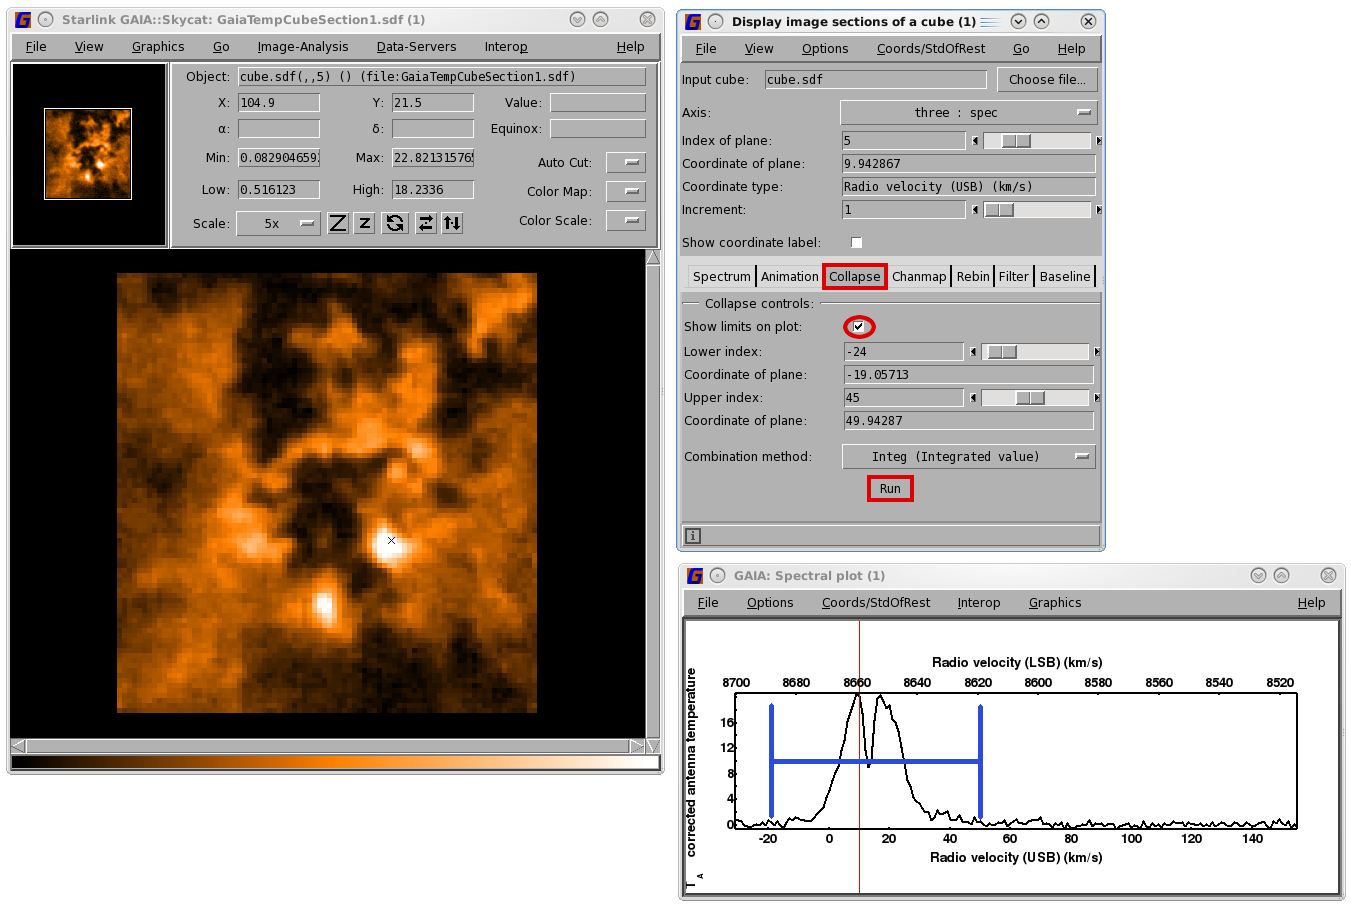
\includegraphics[width=0.9\linewidth]{sc20_gaia_collapse}
\typeout{sc20_gaia_collapse inserted on page \arabic{page}}
\caption[Collapsing your cube using \gaia.]{\label{fig:gaia_collapse}
  Collapsing your cube using \gaia.}
\end{center}
\end{figure}

\section{Three-dimensional visualisation with GAIA}

\begin{enumerate}[label=(\textbf{\arabic*})]
\item Select \guithing{View$>$3D Visualisation$>$Iso
surfaces.../Volume rendering} in the \guiwindow{Display image sections
of a cube} window.

\begin{figure}[h!]
\begin{center}
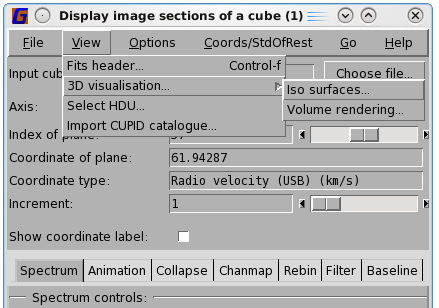
\includegraphics[width=0.45\linewidth]{sc20_gaia_3dmenu}
\typeout{sc20_gaia_3dmenu inserted on page \arabic{page}}
\caption[Selecting the Volume rendering menu in \gaia.]{\label{fig:gaia_3d}
  Selecting the \guithing{Volume rendering} menu in \gaia.}
\end{center}
\end{figure}

\item Click and drag the image display to change the orientation in
the \guiwindow{Volume render} window.

\begin{figure}[h!]
\begin{center}
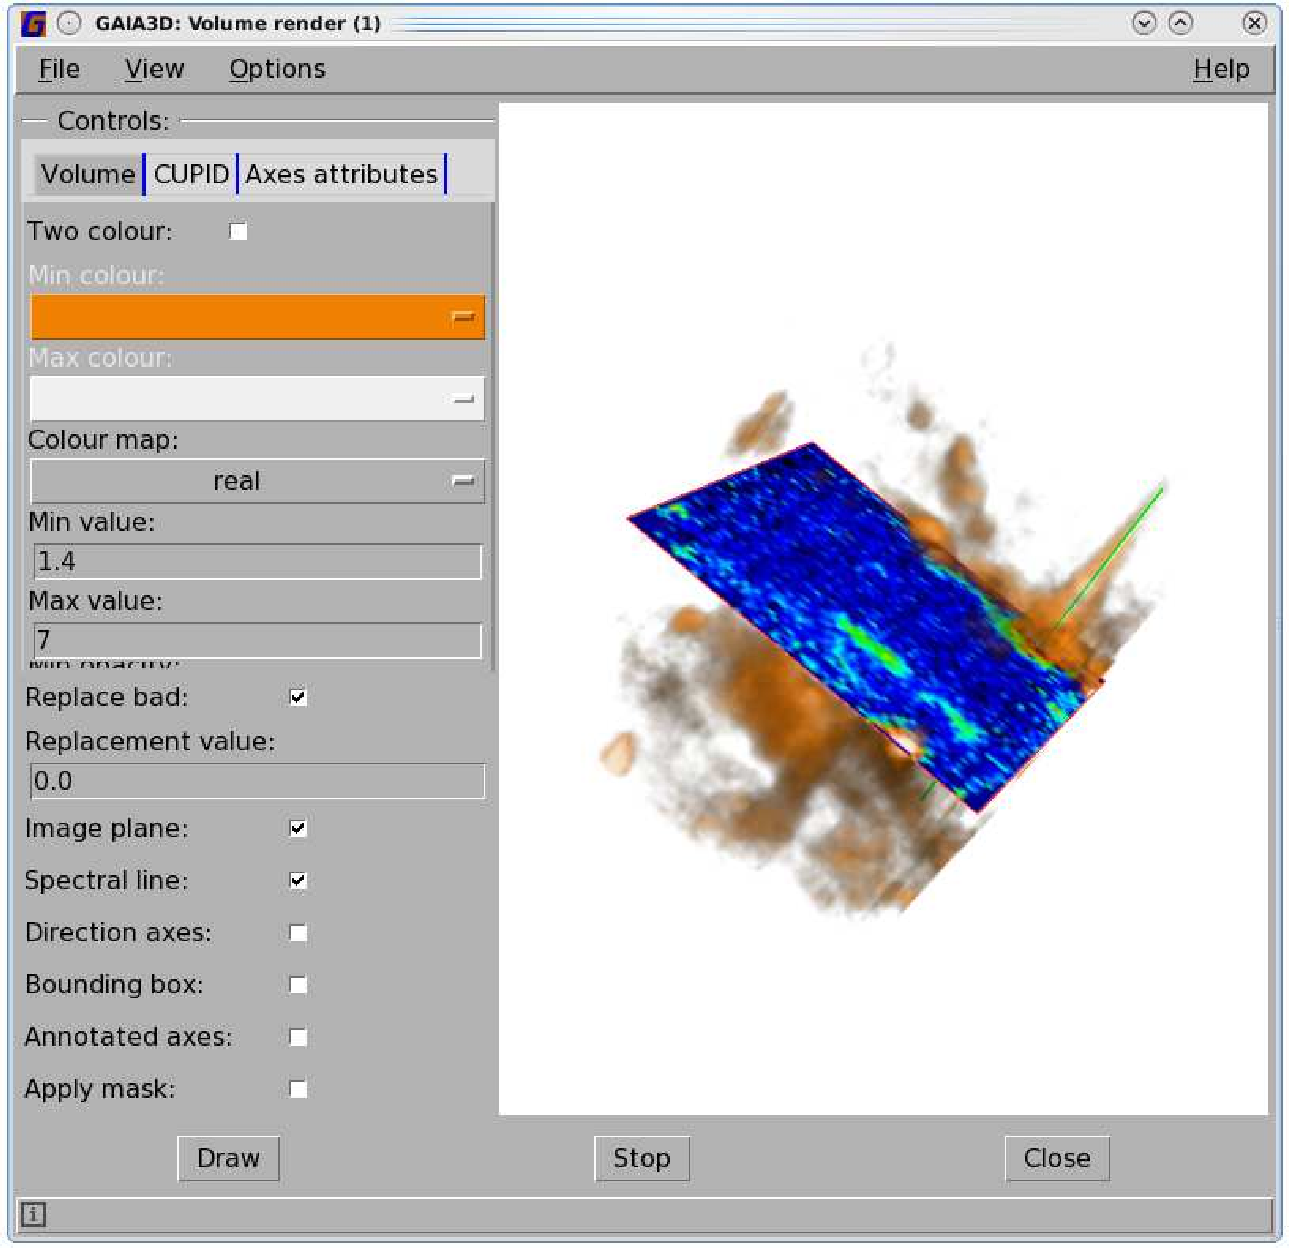
\includegraphics[width=0.6\linewidth]{sc20_gaia-3dvolume2}
\typeout{sc20_gaia-3dvolume2 inserted on page \arabic{page}}
\caption[Three-dimensional visualisation in \gaia.]{\label{fig:gaia_3d2}
  Three-dimensional visualisation in \gaia.}
\end{center}
\end{figure}

\item Include axes labelling, the image plane and other features using
the check boxes on the side bar.
\end{enumerate}


\section{Sending spectra to SPLAT}
\label{sec:gaiatosplat}

\gaia\ has very limited analysis functionality for spectra.  Whereas
\splat\ is a sophisticated graphical spectral-analysis tool. Any
spectrum displayed in \gaia\ (a single-position spectrum or a spectrum
averaged over some region \ref{sec:gaiaaverage}) can be sent (via a
protocol called SAMP) to \splat\ for more-detailed spectral analysis.

\splat\ offers the ability to further process, fit, or identify
spectral lines.  You can also plot different spectra in the same
window and make publishable files.  The full \splat\ documentation can
be found here in \splatsun.

Here are some instructions on how to do this.

\begin{enumerate}[label=(\textbf{\arabic*})]

\item Start \splat, if it is not already running.

\begin{terminalv}
% splat &
\end{terminalv}

\item Click on the \guithing{Interop} menu item in \splat.  If the
\guithing{SAMP control} icon has a red circle, it means that the SAMP
communication hub is running.  If, however, the icon has a white
circle, you need to start a hub.  To do this press the
\guithing{Register with HUB} button at the bottom of the window, and
then press the \guithing{Start internal hub} button in the window that
pops up.

\item If you had \gaia\ already running before the hub was active, then in
\gaia\ select the \guithing{Interop$>$Register} to register your GAIA with
the hub.

\item Select the spectrum you wish to send from \gaia.

\item Click on SPLAT-VO \guithing{Send: replace} or \guithing{Send: add}
button near the bottom of the \guiwindow{Display image sections of a cube}
window.  The spectrum should appear in a \splat\ window.

\end{enumerate}

\begin{figure}[h!]
\begin{center}
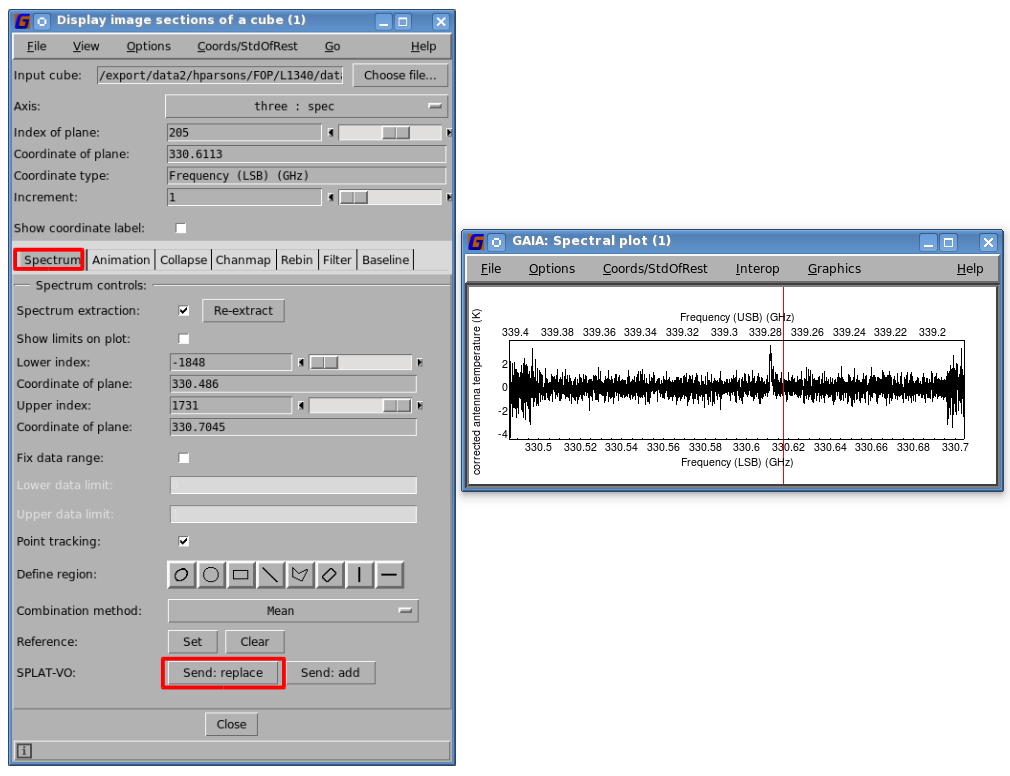
\includegraphics[width=0.9\linewidth]{sc20_gaia_to_splat}
\typeout{sc20_gaia_to_splat inserted on page \arabic{page}}
\caption[Sending spectrum in \gaia\ to \splat.]{\label{fig:gaia_to_splat}
  Sending spectrum in \gaia\ to \splat.}
\end{center}
\end{figure}

SAMP can also transmit images and catalogues between compliant
applications.  For example, you might have a selected catalogue of
sources observed elsewhere in \topcat\ and want to plot the locations
over your HARP maps in \gaia.


\clearpage
\chapter{\xlabel{gaia}Using SPLAT}
\label{sec:splat}

\splat\ is a graphical spectral-analysis tool. \splat\ offers tools for
further processing, fitting, or identification of spectral lines.
One can also plot different spectra in the same window and
make publishable files. The full \splat\ documentation can be found
in \splatsun.

\section{Opening a spectrum in SPLAT}
\label{sec:splat-open}

There are two options for opening up a spectrum in \splat. First it is
possible to send a spectrum to \splat\ using \gaia\ as described in
\cref{Section}{sec:gaiatosplat}{Sending spectra to SPLAT}.

Alternatively spectra can be displayed in directly in \splat\ using:

\begin{terminalv}
% splat filename &
\end{terminalv}

for a single position cube or

\begin{terminalv}
% splat 'filename(xpos,ypos,)' &
\end{terminalv}

to display the spectrum at the pixel position (xpos,ypos). Or simply
initialise \splat\ and open the file directly from the gui.

\begin{terminalv}
% splat  &
\end{terminalv}

When \splat\ is initially started you will get a main window appear
and also a spectral window.

\begin{figure}[h!]
\begin{center}
\includegraphics[width=0.7\linewidth]{sc20_splat_window}
\typeout{sc20_splat_window inserted on page \arabic{page}}
\includegraphics[width=0.6\linewidth]{sc20_splat_spectrum}
\typeout{sc20_splat_spectrum inserted on page \arabic{page}}
\caption[The main \splat\ window and spectrum window.]{\label{fig:splat_window}
  The main \splat\ window and spectral window.}
\end{center}
\end{figure}

\section{Display synopsis of spectrum}
\label{sec:splat-synopsis}

When you initially open a specrum in \splat\ the synopsis of that spectrum
will automatically be overlaid on the spectrum displayed, if the metadata are
known to \splat. The following are a list of possible properties
than can be displayed, with a brief description. Names in parenthesis
are either the FITS keywords or AST attributes used to obtain the values.

\begin{enumerate}
\item  Name: the short name
\item  Telescope: telescope, instrument and its backend
       (\param{TELESCOP}/\param{INSTRUME}/\param{BACKEND})
\item  Object: target, molecule and molecular transition being
       observed (\param{OBJECT}/\param{MOLECULE}/\param{TRANSITI})
\item  Date obs: date of the observation (\param{DATE-OBS} or \att{Epoch} in UTC)
\item  Elevation: observatory elevation (\param{ELSTART} or
       $0.5 * $(\param{ELSTART}$+$\param{ELEND}))
\item  Exposure: exposure time for the spectrum (\param{EXTIME})
\item  Exposure (median): exposure time for the spectrum (\param{EXP\_TIME})
\item  Exposure (elapsed): the time elapsed during exposure (\param{INT\_TIME}
       otherwise \param{DATE-END} $-$ \param{DATE-OBS})
\item  Exposure (effective): effective exposure time (\param{EXEFFT})
\item  Coords sys: the co-ordinate system code (\att{System})
\item  Spec position: position of spectrum on the sky (\param{EXRAX}, \param{EXDECX})
\item  Src position: position of the observation centre (\param{EXRRA}, \param{EXRDEC})
\item  Img centre: centre of the originating image (\param{EXRA}, \param{EXDEC})
\item  Offset: offset of spectrum from the observation centre
       (\param{EXRRAOF}, \param{EXRDECOF} or \param{EXRAOF}, \param{EXDECOF})
\item  Doppler RA Dec: reference position (\att{RefRA},\att{RefDec})
\item  SourceVel: source velocity (\att{SourceVel})
\item  SourceVRF: source velocity reference frame (\att{SourceVRF})
\item  SourceSys: system of the source velocity (\att{SourceSys})
\item  StdOfRest: standard of rest (\att{StdOfRest})
\item  RestFreq: rest frequency (\att{RestFreq}
\item  ImageFreq: image sideband equivalent of the rest frequency (\att{ImagFreq})
\item  Channel spacing: channel spacing (derived value)
\item  Number of channels: Number of co-ordinate positions
\item  TSYS: system temperature (\param{TSYS})
\item  TSYS (median): median system temperature (\param{MEDTSYS})
\item  TSYS (est): system temperature (derived value)
\item  TRX: receiver temperature (\param{TRX})
\end{enumerate}

To show or remove the synopsis of a spectrum simply click on the
\guithing{Options} button in the spectral view window and select or deselect
\guithing{Display Synopsis}. To move the position of the synopsis simply click
and drag the text box to the desired location.

\begin{figure}[h!]
\begin{center}
\includegraphics[width=0.8\linewidth]{sc20_splat_display_synopsis}
\typeout{sc20_splat_display_synopsis inserted on page \arabic{page}}
\caption[Display or remove the spectral synopsis.]{\label{fig:splat_synopsis}
  How to display or remove the synopsis of a spectrum in the spectral
  window.}
\end{center}
\end{figure}

\section{Changing units of a spectrum in SPLAT}
\label{sec:splat-units}

Sometime you may wish to change the units of a spectrum in \splat.


\begin{enumerate}[label=(\textbf{\arabic*})]

\item Click on \guithing{Change the units of the current spectrum}
button in your current spectral window.


\item A new window will appear called \guiwindow{Current Spectrum Units}.

\begin{figure}[h!]
\begin{center}
\includegraphics[width=0.9\linewidth]{sc20_splat_spectrum_units}
\typeout{sc20_splat_spectrum_units inserted on page \arabic{page}}
\includegraphics[width=0.7\linewidth]{sc20_splat_spectrum_units2}
\typeout{sc20_splat_spectrum_units2 inserted on page \arabic{page}}
\caption[Change the units of the current spectrum.]{\label{fig:splat_units1}
  Top: Select the \guithing{Change the units of the current spectrum}
  button. Note that in this example the current units are Frequency.
  Bottom: the \guiwindow{Current Spectrum Units} window.}
\end{center}
\end{figure}


\item From the Coordinates drop-down menu select the desired unit
(in this case we select \guithing{Kilometers-per-sec (radio)}).
Then click \guithing{Apply}.

\begin{figure}[h!]
\begin{center}
\includegraphics[width=0.7\linewidth]{sc20_splat_spectrum_units3}
\typeout{sc20_splat_spectrum_units3 inserted on page \arabic{page}}
\caption[Changing the units via the drop-down menu.]{\label{fig:splat_units2}
  Changing the units of the spectrum via the drop-down menu to \kms.}
\end{center}
\end{figure}

\item You will now see that the spectrum is
displayed in \guithing{Radio Velocity (km/s)}.

\begin{figure}[h!]
\begin{center}
\includegraphics[width=0.9\linewidth]{sc20_splat_spectrum_units4}
\typeout{sc20_splat_spectrum_units4 inserted on page \arabic{page}}
\caption[Spectrum with units of \kms.]{\label{fig:splat_units3}
  Spectrum with units of \kms.}
\end{center}
\end{figure}

\end{enumerate}


\section{Cropping a spectrum in SPLAT}
\label{sec:splat-crop}


\begin{enumerate}[label=(\textbf{\arabic*})]

\item Click on \guithing{Cut out the regions of the current spectrum} button
above the spectrum you wish to work on. This will open a new window.


\item Select \guithing{Add} from the cut region window.

\begin{figure}[h!]
\begin{center}
\includegraphics[width=0.7\linewidth]{sc20_splat_tocut_spectrum}
\typeout{sc20_splat_tocut_spectrum inserted on page \arabic{page}}
\includegraphics[width=0.65\linewidth]{sc20_splat_cutregion_blank}
\typeout{sc20_splat_cutregion inserted on page \arabic{page}}
\caption[Select the crop button in SPLAT.]{\label{fig:splat_crop1}
  Top: Select the cut button. Bottom: Select the \guithing{Add} button.}
\end{center}
\end{figure}


\item Click and drag the regions you wish to remove from the
spectrum in the spectrum window. As we had a
second region to remove we click on the \guithing{Add} button
a second time. In this example we select the two noisy edge regions from the
spectrum to remove.


\item Select the \guithing{Remove Selected} button.

\begin{figure}[h!]
\begin{center}
\includegraphics[width=0.7\linewidth]{sc20_splat_cutregion2}
\typeout{sc20_splat_cutregion inserted on page \arabic{page}}
\includegraphics[width=0.65\linewidth]{sc20_splat_cutregion}
\typeout{sc20_splat_cutregion2 inserted on page \arabic{page}}
\caption[Selected regions for removal.]{\label{fig:splat_crop2}
  Top: The two regions selected. Bottom: remove the selected region
  by clicking the \guithing{Remove Selected} button.}
\end{center}
\end{figure}


\item A new spectrum with the noisy edges removed will now appear
in the main \splat\ window. Click on your newly created spectrum
to view.

\begin{figure}[h!]
\begin{center}
\includegraphics[width=0.65\linewidth]{sc20_splat_window_main_cut}
\typeout{sc20_splat_window_main_cut inserted on page \arabic{page}}
\includegraphics[width=0.7\linewidth]{sc20_splat_cut_spectrum}
\typeout{sc20_splat_cut_spectrum inserted on page \arabic{page}}
\caption[Spectrum with noisy edges removed.]{\label{fig:splat_crop5}
  Top: Select the newly created spectrum in the main \splat\ window.
  The spectrum with the selected noisy-edge-data removed will then appear. }
\end{center}
\end{figure}

\end{enumerate}

\section{Rebinning a spectrum in SPLAT}
\label{sec:splat-rebin}


\begin{enumerate}[label=(\textbf{\arabic*})]

\item Click on \guithing{Apply a filter to the current spectrum} button
above the spectrum you wish to work on. This will open a new window.

\item Select the number of channels over which you want to
bin---this is the \guithing{Width}.
In this example the spectrum has a resolution of 0.055\kms. We
bin by 18 channels to rebin the spectrum to 1\kms\ channels.

\item Select \guithing{Filter (Replace)}. This will create a
new spectrum in the main \splat\ window and will also replace the
existing spectrum displayed in the spectral window with the new
binned spectrum.

\begin{figure}[h!]
\begin{center}
\includegraphics[width=0.6\linewidth]{sc20_splat_rebin}
\typeout{sc20_splat_rebin inserted on page \arabic{page}}
\includegraphics[width=0.7\linewidth]{sc20_splat_rebin2}
\typeout{sc20_splat_rebin2 inserted on page \arabic{page}}
\caption[Filter regions of a spectrum window.]{\label{fig:splat_rebin}
  Top: The \splat\ \guiwindow{Filter regions of a spectrum} window.
  Bottom: The final rebinned spectrum.}
\end{center}
\end{figure}


\end{enumerate}


\section{Estimating the noise in a spectrum using SPLAT}
\label{sec:splat-stats}

\begin{enumerate}[label=(\textbf{\arabic*})]

\item Click on \guithing{Get statistics on region of spectrum}
button above the spectrum you wish to work on. This will open a
new window.


\item Select \guithing{Add} from the \guiwindow{Region statistics} window.

\begin{figure}[h!]
\begin{center}
\includegraphics[width=0.75\linewidth]{sc20_splat_stats}
\typeout{sc20_splat_stats inserted on page \arabic{page}}
\includegraphics[width=0.6\linewidth]{sc20_splat_stats1}
\typeout{sc20_splat_stats1 inserted on page \arabic{page}}
\caption[Select the statistics button.]{\label{fig:splat_stats1}
  Top: Select the statistics button. Bottom: Select the \guithing{Add}
  button.}
\end{center}
\end{figure}

\item Click and drag the regions you calculate the statistics over.
As we wish to include baselines eithersie of the spectral line seen
in the data we click on the \guithing{Add} button a second time.

\begin{figure}[h!]
\begin{center}
\includegraphics[width=0.75\linewidth]{sc20_splat_stats2}
\typeout{sc20_splat_stats2 inserted on page \arabic{page}}
\caption[Select region for statistics.]{\label{fig:splat_stats2}
  Click and drag the regions over which you wish to estimate the noise.}
\end{center}
\end{figure}

\item You will see the two selected spectral regions appear in
a table in the \guiwindow{Region statistics} window with some
basic statistic already computed for each region created.

\begin{figure}[h!]
\begin{center}
\includegraphics[width=0.75\linewidth]{sc20_splat_stats3}
\typeout{sc20_splat_stats3 inserted on page \arabic{page}}
\caption[Two spectral regions have been selected.]{\label{fig:splat_stats3}
  Two spectral regions have been selected and are displayed
  in the \guiwindow{Region statistics} window.}
\end{center}
\end{figure}

\item Click on \guithing{Selected stats} or \guithing{All stats}
to get statistics of the regions combined. In this example we see the
standard deviation in the regions selected is 0.19K.

\begin{figure}[h!]
\begin{center}
\includegraphics[width=0.75\linewidth]{sc20_splat_stats4}
\typeout{sc20_splat_stats4 inserted on page \arabic{page}}
\caption[statistics for both regions.]{\label{fig:splat_stats4}
  Statistics for both regions are displayed in the \guiwindow{Region
  statistics} window. }
\end{center}
\end{figure}


\end{enumerate}


\section{Fitting a line in a spectrum using SPLAT}
\label{sec:splat-fit}

Your data might have lines for which you want a quick estimate of its
line strength and width.


\begin{enumerate}[label=(\textbf{\arabic*})]


\item Click on \guithing{Fit spectral lines using a variety of functions}
button above the spectrum you wish to work on. This will open a
new window.

\item Click on the \guithing{Add} button in the
\guiwindow{Measure spectral lines} window.


\begin{figure}[h!]
\begin{center}
\includegraphics[width=0.7\linewidth]{sc20_splat_fit1}
\typeout{sc20_splat_fit1 inserted on page \arabic{page}}
\includegraphics[width=0.45\linewidth]{sc20_splat_fit2}
\typeout{sc20_splat_fit2 inserted on page \arabic{page}}
\caption[Select the SPLAT fit button.]{\label{fig:splat_fit1}
  Top: Select the spectral-fitting button. Bottom: Click on
  the \guithing{Add} button.}
\end{center}
\end{figure}


\item Click and drag the box that appears in the spectral window
to encompass the line for which you wish to calculate a fit for.


\begin{figure}[h!]
\begin{center}
\includegraphics[width=0.7\linewidth]{sc20_splat_fit3}
\typeout{sc20_splat_fit3 inserted on page \arabic{page}}
\caption[Spectral fit region defined.]{\label{fig:splat_fit3}
  Click and drag the region containing the line which you wish
  to be fitted.}
\end{center}
\end{figure}


\item Click on the \guithing{Fit} button to produce both a
\guithing{Quick} and \guithing{Gaussian} fit to the spectral line.

\begin{figure}[h!]
\begin{center}
\includegraphics[width=0.45\linewidth]{sc20_splat_fit4}
\typeout{sc20_splat_fit4 inserted on page \arabic{page}}
\caption[Getting the spectral line fit.]{\label{fig:splat_fit4}
  In the \guiwindow{Measure spectral lines} window, we see the both
  the \guithing{Quick} fit (black dashed line) and the
  \guithing{Gaussian} fit (pink line) of the spectral line.}
\end{center}
\end{figure}


\item We see the results of the fit are provided in the
\guiwindow{Measure spectral lines} window, and the two fits can
be seen in the spectral line window.

\begin{figure}[h!]
\begin{center}
\includegraphics[width=0.9\linewidth]{sc20_splat_fit5}
\typeout{sc20_splat_fit5 inserted on page \arabic{page}}
\caption[Spectrum with fits.]{\label{fig:splat_stats5}
  In the spectral window we see the both the \guithing{Quick}
  fit (black dashed line) and the \guithing{Gaussian} fit
  (pink line) of the spectral line.}
\end{center}
\end{figure}





\end{enumerate}



\clearpage
\chapter{\xlabel{cadc}Getting your data from CADC}
\label{sec:fromcadc}

The JCMT Science Archive is hosted by The Canadian Astronomy Data
Centre (CADC). Both raw data and data processed by the science pipeline
are made available to PIs and co-Is through the CADC Advanced Search
interface linked from the JCMT landing page
(\url{http://www3.cadc-ccda.hia-iha.nrc-cnr c.gc.ca/jcmt/}).

To access proprietary data you will need to have your CADC username
registered by the EAO and thereby associated with the project code.

When searching the JCMT Science Archive, be sure to select the correct
search option from the `JSA Queries' tab. Here you can select public
versus proprietary, raw versus reduced, and SCUBA-2 versus ACSIS data.

\begin{figure}[b!]
\begin{center}
\includegraphics[width=0.98\linewidth]{sc20_cadc}
\caption{\label{fig:cadc}
  Screenshot of the CADC search window for reduced HARP data.}
\end{center}
\end{figure}

An important search option to be aware of is `Group Type', where your
options are Simple, Night, Project and Public. Simple (which becomes
`obs' on the result page) is an individual observation; night means
the group file from the pipeline (these may or may not include more
than one observation; the `Group Members' value will tell you); and the
project option is generated if an entire project has been run through
the pipeline and identical sources across the project are co-added
into master group files.

The format and file naming conventions are different in the JSA for
\emph{reduced} data compared with merely running \ORACDR.  Reduced
observations will be in FITS format with the \file{.fits} file
extension.  File names begin with the \file{jcmth} prefix followed by
the UT date, observation number, subsystem number, the product name
and subscan number, the grouping algorithm, and finally a version
number (in practice zero), with adjacent elements separated by an
underscore.  The product name of most interest will be \file{reduced},
but others include \file{rimg} and \file{rsp} for the representative
image and spectrum.  The grouping algorithm is \file{obs} for a single
observation, and \file{nit} where all the good data for an object observed
with the same instrumental setup during a night are combined to create
products of better quality.  A further grouping is \file{pro}) where
matching observations within a project are combined, which may extend
over many nights spanning years.

Here is are some examples:
\file{jcmth20070728\_00066\_01\_reduced002\_obs\_000.fits}, \\
\file{jcmth20070728\_00066\_01\_rimg001\_nit\_000.fits}, and
\file{jcmth20070728\_00066\_02\_rsp001\_pro\_000.fits}.

For a detailed guide to using the Advanced Search see
\htmladdnormallink{JSA User's Guide}{http://www.eaobservatory.org/jcmt/science/archive/guide/}.


\clearpage

\begin{thebibliography}{}
\addcontentsline{toc}{section}{References}

\bibitem{cupid}
Berry~D.~S., 2013, \textit{CUPID. Version 2.0}, \xref{Starlink User Note 255}{sun255}{}

\bibitem{fellwalker}
Berry~D.~S., 2015, \htmladdnormallink{\textit{FellWalker---a clump-identification
algorithm}}{https://doi.org/10.1016/j.ascom.2014.11.004}, Astronomy and Computing,
10, 22 (DOI:10.1016/j.ascom.2014.11.004)

\bibitem{harp}
Buckle, J.~V., Hills, R.~E., Smith, H., et al., 2009, \htmladdnormallink{
\textit{HARP/ACSIS: a submillimetre spectral imaging system on the James Clerk Maxwell Telescope}}
{https://doi.org/10.1111/j.1365-2966.2009.15347.x}, MNRAS, 399, 1026
(DOI:10.1111/j.1365-2966.2009.15347.x)

\bibitem{oracdr}
Cavanagh~B., Jenness~T., Economou~F., Currie~M.~J., 2008,
\htmladdnormallink{\textit{The ORAC-DR data reduction pipeline}}{https://doi.org/10.1002/asna.200710944},
Astron. Nactr., 329, 295 (DOI:10.1002/asna.200710944)

\bibitem{smurf}
Chapin~E.~L., et~al., 2013, \textit{SMURF -- Sub-Millimetre User Reduction
Facility}, \xref{Starlink User Note 258}{sun258}{}

\bibitem{convert}
Currie~M.~J., Privett~G.~J., Chipperfield~A.~J., Berry~D.~S. and Davenhall~A.C., 2013,
\textit{CONVERT -- A Format-conversion Package}, \xref{Starlink User Note 55}{sun55}{}

\bibitem{ssds}
Currie~M.~J., Wallace~P.~T., Warren-Smith~R.~F., 1989,
\textit{Starlink Standard Data Structures}, \xref{Starlink General
Paper 38.2}{sgp38}{}

\bibitem{kappa}
Currie~M.~J., Berry~D.~S, 2013, \textit{KAPPA -- Kernel Application Package},
\xref{Starlink User Note 95}{sun95}{}

\bibitem{flat}
Curtis~E.~I., Richer~J.~S. and Buckle~J.~V. 2010, \htmladdnormallink{\textit{A submillimetre
survey of the kinematics of the Perseus molecular cloud -- I.
Data}}{https://doi.org/10.1111/j.1365-2966.2009.15658.x},
MNRAS, 401, 455 (DOI:10.1111/j.1365-2966.2009.15658.x)

\bibitem{gaia}
Draper~P.~W., Gray~N., Berry~D.~S., Taylor~M., 2012,
\textit{GAIA -- Graphical Astronomy and Image Analysis Tool},
\xref{Starlink User Note 214}{sun214}{}

\bibitem{ccdpack}
Draper~P.~W., Taylor~M. and Allan~A., 2011, \textit{CCDPACK -- CCD data reduction package},
\xref{Starlink User Note 139}{sun139}{}

\bibitem{picard}
Gibb~A.~G., Jenness~T., Economou~F., 2012, \textit{PICARD --- a
PIpeline for Combining and Analyzing Reduced Data},
\xref{Starlink User Note 265}{sun265}{}

\bibitem{oracdr_infra}
Jenness~T. \& Economou~F., 2015,
\htmladdnormallink{\textit{ORAC-DR: A generic data reduction pipeline
infrastructure}}{http://dx.doi.org/10.1016/j.ascom.2014.10.005}, Astronomy and
Computing, 9, 40 (DOI:10.1016/j.ascom.2014.10.005)

\bibitem{heterodyne_pipeline}
Jenness~T., Currie~M.~J., Tilanus~R., Cavanagh~B., Berry~D.~S.,
Leech~J., Rizzi~L., 2015, \htmladdnormallink{\textit{Automated reduction of
sub-millimetre single-dish heterodyne data from the James Clerk
Maxwell Telescope using ORAC-DR}}{http://dx.doi.org/10.1093/mnras/stv1545},
MNRAS, 453, 73 (DOI:10.1093/mnras/stv1545)

\end{thebibliography}

\newpage
\appendix

\chapter{PICARD}
\label{app:picard}
There are two \picard\ recipes which can be used with ACSIS data and are of general interest:

\section{CREATE\_MOMENTS\_MAP}

This recipe is used to create a moments maps from a cube. It smooths
the cube in frequency and spatial extents, then uses the ClumpFind
algorithm to find clumps of emission. Everything in the cube not found
in a clump is masked out, then the masked cube is collapsed to form
the moments map.
\\\\
\textbf{Recipe options:}
\begin{itemize}

\item BASELINE\_ORDER: The polynomial order for baseline fitting
\param{[1]}

\item CLUMP\_METHOD: Method to find emission in the data
(\param{clumpfind}/\param{fellwalker}/\param{thresh}) \param{[clumpfind]}

\item FREQUENCY\_SMOOTH: Smoothing kernel size in channels along the
frequency axis for baseline determination \param{[25]}

\item MOMENTS:  Which moments maps to create (\param{integ}/\param{iwc}/\param{itd})
\param{[integ]}

\item MOMENTS\_LOWER\_VELOCITY: An optional lower velocity in \kms, below which
no data will be used when creating the moments map \param{[undef]}

\item MOMENTS\_UPPER\_VELOCITY: An optional upper velocity in \kms, above which
no data will be used when creating the moments map \param{[undef]}

\item MOMENTS\_SNR: Selects whether or not to do clump detection on an
signal-to-noise cube instead of the signal cube. Enabling this is
useful for data taken in varying conditions. \param{[0]}

\item SPATIAL\_SMOOTH: Smoothing kernel size in pixels along both
spatial axes for baseline determination \param{[3]}
\end{itemize}


\section{MOSAIC\_JCMT\_IMAGES}

This recipe co-add the given files into a single map while correctly
handling the exposure time FITS header and other NDF components. The
maps are combined using inverse-variance weighting and the output
variance is derived from the input variances. You can choose either
\wcsmosaic\ or a combination of \wcsalign\ and the \ccdpack\
application \makemos\ to mosaic the images.
\\\\
\textbf{Recipe options:}
\begin{itemize}
\item MOSAIC\_EACH: Flag to indicate whether the data should be
mosaicked by individual object or combined into a single output file.
\item MOSAIC\_TASK: Name of mosaicking task to use, \wcsmosaic\ or
\makemos. \param{[wcsmosaic]}
\item MAKEMOS\_METHOD: Image combination method for \makemos, may be
\param{median} (default), \param{mean} or \param{sigmas}. See \xref{\textsc{ccdpack}
manual}{sun139}{} for advice on choosing a method.
\item MAKEMOS\_SIGMAS: Sigma-clipping threshold if MAKEMOS\_METHOD =
sigmas. \param{[4]}
\item MASK\_LOWVAR: Flag to indicate that pixels with anomalously-low
variances should be removed before mosaicking. \param{[0]}
\item WCSMOSAIC\_METHOD: \wcsmosaic\ and \wcsalign\ pixel-spreading
method. \param{[nearest]}
\item WCSMOSAIC\_PARAMS: additional parameters that may be specified
with \wcsmosaic.

\end{itemize}


\section{Running PICARD recipes}

There are a number of options available when running \picard\ recipes.
The example below illustrates most of them.
\begin{terminalv}
% picard -recpars params.ini MOSAIC_JCMT_IMAGES `cat myfilelist.lis` -log sfx
\end{terminalv}

\begin{itemize}
\item The recipe parameters are listed in a file called \file{params.ini}.
It is called by the \param{recpars} option. This file has the same
\file{.ini} format used by the \ORACDR\ pipeline (see
\cref{Section}{sec:recpars}{Setting recipe parameters}).
\item The recipe name need to be in uppercase.
\item If you need to supply multiple files you can do so by listing
them in a file (\file{myfilelist.lis} in this example) and running cat on it.
The input file must be in the current directory, or a directory
defined by the environment variable \file{ORAC\_DATA\_IN}. Note the
back-quotes.
\item Like the \ORACDR\ pipeline, the \param{-log} option specifies
whether the log file should be written to the screen [\param{s}], a
file [\param{f}] or an xwindow [\param{x}].
\end{itemize}

\begin{tip}
TIP: The \file{.sdf} extension on filenames is required by \textsc{Picard}.
\end{tip}

\begin{tip}
If the environment variable \envvar{ORAC\_DATA\_OUT} is defined, any files
created by \textsc{Picard} will be written in that location. Check there if new
files are expected but do not appear in your working directory.
\end{tip}

\newpage
\chapter{\xlabel{convert}Converting file formats}
\label{app:convert}

\section{Converting a FITS file to NDF}

A FITS file can be converted to NDF using the \starlink\ package
\convert.  The \texttt{convert} instruction sets up the definitions
for this package and only needs to be entered once,

\begin{terminalv}
% convert
\end{terminalv}

the relevant one here being \texttt{fits2ndf}.

\begin{terminalv}
% fits2ndf file.fits file.sdf
\end{terminalv}

Note that the \file{.sdf} file extension NDF may be omitted to save
typing.

Unless your FITS file is from a recognised source, \fitstondf\ puts the
various FITS extensions into NDF extensions called FITS\_EXT\_$<\!n\!>$,
where $n$ counts from one for the first FITS extension. These are
located in the top-level MORE component of the NDF. If one of these is
the array you want---it should be an NDF too---it will be easier to
handle if you copy out of the NDF extension to its own NDF.

\begin{terminalv}
% ndfcopy in=file.more.fits_ext_1 out=file_data
\end{terminalv}

If there is a variance array stored in another extension that you want
to attach to your new NDF, a command like the following will do that.

\begin{terminalv}
% setvar ndf=file_data from=file.more.fits_ext_2
\end{terminalv}

\task{fits2ndf} does offer a way of mapping FITS extensions to familiar NDF
array components DATA, VARIANCE, and QUALITY through the \param{EXTABLE} file,
avoiding the \ndfcopy\ and possible \setvar\ steps.

\section{Converting an NDF file to FITS}

The \convert\ package can also be used to convert an NDF file to FITS format.

\begin{terminalv}
% convert
% ndf2fits file file.fits
\end{terminalv}

There are options to control whether or not to export all of the NDF
extensions (\param{PROEXTS}) and history records (\param{PROHIS}),
and whether or not to merge the contents of the FITS airlock
(\param{PROFITS}).

For historical reasons the specific set of headers encoding the world
co-ordinate system varies from package to package.  There is a parameter
to select the appropriate encoding for the destination of the FITS file.
A common one in the submillimetre world is the \textsc{Class} package used
for spectroscopic reductions.

\begin{terminalv}
% ndf2fits ga20091011_37_1_reduced \* encoding=fits-class
\end{terminalv}

This will create a \file{ga20091011\_37\_1\_reduced.fit} file with the
\textsc{Class}-style of WCS headers.

\newpage
\chapter{\xlabel{script}Scripting your reduction}
\label{app:script}

You may wish to write a script to process your data rather than
running each task independently. In this case your script should start
with:
\begin{terminalv}
#!/bin/csh -f
source $STARLINK_DIR/etc/login >& /dev/null
source $STARLINK_DIR/etc/cshrc >& /dev/null
kappa >& /dev/null
\end{terminalv}


\chapter{\xlabel{regrid}Regridding versus resampling}
\label{app:regrid}

Sometimes you may wish to put your data onto a new pixel-size scheme.
This may either involve regridding (often called rebinning) the data
onto larger pixel sizes, or resampling the data onto smaller pixels,
both using \Kappa.

The key difference between rebinning and resampling is whether you
iterate over the input or output pixels.  Rebinning divides each input
pixel value between a group of neighbouring output pixels, whereas
resampling allocates each output pixel a value sampled from the input
array.

\begin{figure}[h!]
\begin{center}
\includegraphics[width=0.8\linewidth]{sc20_regrid}
\caption{\label{fig:regrid}
  Regridding versus resampling.}
\end{center}
\end{figure}

\emph{resampling}---Resampling of the grid of input data is performed
by transforming the co-ordinates of the centre of each output pixel
into the co-ordinate system of the input grid. Since the resulting
co-ordinates will not, in general, coincide with the centre of an
input pixel, sub-pixel interpolation is performed between the
neighbouring input pixels. This produces a resampled value, which is
then assigned to the output pixel.  Since resampling does not
integrate, the total data value in the input image will not, in
general, be conserved.  Resampling has the advantage of ensuring that
the output image is filled (provided the input array contains good
data).


\emph{rebinning}---Rebinning of the grid of input data is performed by
transforming the co-ordinates of the centre of each input pixel
into the co-ordinate system of the output grid.
The input pixel value is then divided up and assigned to the
output pixels in the neighbourhood of the central output
co-ordinates. A choice of schemes are provided for determining
how each input pixel value is divided up between the output
pixels. In general, each output pixel may be assigned values
from more than one input pixel. All contributions to a given
output pixel are summed to produce the final output pixel value.
Rebinning can leave gaps in the output array if the output
array's pixels are smaller than those of the input array.

\newpage
\chapter{\xlabel{clumpfind}Clump-finding Algorithms}
\label{app:clumpfind}

\textbf{GaussClumps}\\Based on the algorithm described by Stutzki \&
G\"{u}sten (1990, ApJ 356, 513). This algorithm proceeds by fitting a
Gaussian profile to the brightest peak in the data. It then subtracts
the fit from the data and iterates, fitting a new ellipse to the
brightest peak in the residuals. This continues until the integrated
data sum in the fitted Gaussians reaches the integrated data sum in
the input array, or a series of consecutive fits are made which have
peak values below a given multiple of the noise level. Each fitted
ellipse is taken to be a single clump and is added to the output
catalogue. In this algorithm, clumps may overlap. Any input variance
component is used to scale the weight associated with each pixel value
when performing the Gaussian fit. The most significant configuration
parameters for this algorithm are: \param{GaussClumps.FwhmBeam} and
\param{GaussClumps.VeloRes} which determine the minimum clump size.
\\\\
\textbf{ClumpFind}\\
Described by Williams et al (1994, ApJ 428, 693). This algorithm works
by first contouring the data at a multiple of the noise, then searches
for peaks of emission which locate the clumps, and then follows them
down to lower intensities. No a priori clump profile is assumed. In
this algorithm, clumps never overlap. Clumps which touch an edge of
the data array are not included in the final list of clumps.
\\\\
\textbf{Reinhold}\\
Based on an algorithm developed by Kim Reinhold at JAC. See
\cupidsun\ for more information on this algorithm. The edges of the
clumps  are first found by searching for peaks within a set of
one-dimensional profiles running through the data, and then following
the wings of each peak down to
the noise level or to a local minimum. A mask is thus produced in
which the edges of the clumps are marked. These edges however tend to
be quite noisy, and so need to be cleaned up before further use. This
is done using a pair of cellular automata which first dilate the edge
regions and then erode them. The volume between the edges are then
filled with an index value associated with the peak position. Another
cellular automata is used to removed noise from the filled clumps.
\\\\
\textbf{FellWalker}\\
David Berry devised an algorithm\cite{fellwalker} that walks up hills along the line
of greatest gradient until a significant peak is reached. It then
assigns all pixels visited along the route to the clump associated with the peak.
Such a walk is performed for every pixel in the data array which is
above a specified background level.
\\\\
See \cupidsun\ for more information on \findclumps\ and a full list of
the configuration options for each algorithm.


\newpage
\chapter{\xlabel{display}Viewing your data with KAPPA}
\label{app:display}

This appendix offers a few examples of creating different types of
plots using \Kappa. The applications highlighted here are \display\
and \contour\ for maps, and \linplot\ and \clinplot\ for spectra (See
the \xref{\textsc{Kappa} manual}{sun95}{} for more details).

The plotting attributes for each of these applications is controlled
in the same way.  For full details of all the formatting options as
well as setting up your graphics device, see the `Plotting Styles and
Attributes' section in the \xref{\textsc{Kappa} manual}{sun95}{}.

\section{Setting up xwindows}
\begin{itemize}
\item Clear my graphics window and reset default values.
\begin{terminalv}
% gdclear
\end{terminalv}
\item Set my display device to xwindows.
\begin{terminalv}
% gdset xw
\end{terminalv}
\item Create an xwindow of the desired dimensions.
\begin{terminalv}
% xmake -width 1500 -height 1000 xwindows
\end{terminalv}
\item To create a display window which plots black on a white
background, change the order of black and white in the palette list
for your graphics device. Check this using \gdstate.
\begin{terminalv}
% gdstate
\end{terminalv}
Ensure white is entry 0 and black in entry 1.
\begin{terminalv}
% palentry 0 White
% palentry 1 Black
\end{terminalv}
\end{itemize}

\section{Format axes}
\begin{itemize}
\item Use \wcsattrib\ to set how your axes should be formatted. Here
the format of the first and second axes is set to two decimal places
for Galactic co-ordinates. Find out more about the \att{Format} attribute
under \wcsattrib\ in the \xref{\textsc{Kappa} manual}{sun95}{}.
\begin{terminalv}
% wcsattrib map set format"(1)" .2
% wcsattrib map set format"(2)" .2
\end{terminalv}

\item For FK5 co-ordinates you can use the same method to set exactly
how the co-ordinates should be displayed. The example below sets R.A.
units to $0^h00^m00^s$ and Dec. units to $00'00''$.
\begin{terminalv}
% wcsattrib fk5map set format"(1)" ghms
% wcsattrib fk5map set format"(2)" gdms
\end{terminalv}
\end{itemize}

\newpage

\section{Plotting a two-dimensional image}

\begin{itemize}
\item Display \file{map.sdf}. Do draw axes and a border, but do not draw a
title or a grid. The default cut parameters for \param{mode=scale}
include all the data.
\begin{terminalv}
% display map border axes style='"drawtitle=0,grid=0"' mode=scale
\end{terminalv}
Depending on your default settings you may get a map like the one below.

\begin{figure}[h!]
\begin{center}
\includegraphics[width=0.475\linewidth]{sc20_display1}
\typeout{sc20_display1 inserted on page \arabic{page}}
\caption[First attempt at displaying an integrated map with \Kappa:\display.]{\label{fig:display1}
  First attempt at displaying an integrated map with \Kappa:\display.}
\end{center}
\end{figure}

\item Re-draw calling a style file and changing the scaling.
\begin{terminalv}
% display integ.sdf axes style=^style.dat mode=scale low=0 high=100
\end{terminalv}

\begin{figure}[h!]
\begin{center}
\includegraphics[width=0.475\linewidth]{sc20_display2}
\typeout{sc20_display2 inserted on page \arabic{page}}
\caption[Displaying an integrated map with \Kappa:\display\ using a style file.]{\label{fig:display2}
  Displaying an integrated map with \Kappa:\display\ using a style file
  to format the plotting attributes.}
\end{center}
\end{figure}

Below is a copy of the style file (\file{style.dat}) used to make
\cref{Figure}{fig:display2}{the figure above}.

\begin{terminalv}
border=1
tickall=1
majticklen=0.01
drawtitle=0
color(axis)=white
color(numlab)=black
color(border)=black
color(ticks)=white
size(numlab)=1
size(textlab)=1.5
nogrid=1
textlabgap(1)=0.01
textlabgap(2)=0.01
\end{terminalv}

\item Make the colour scale negative and then replot.
\begin{terminalv}
% lutneg
% display integ.sdf axes style=^style.dat mode=scale low=0 high=100
\end{terminalv}

\begin{figure}[h!]
\begin{center}
\includegraphics[width=0.47\linewidth]{sc20_display9}
\typeout{sc20_display9 inserted on page \arabic{page}}
\caption[Reversing the colour scale in \Kappa:\display.]{\label{fig:display9}
  Reversing the colour scale in \Kappa:\display.}
\end{center}
\end{figure}

\item There are a number of colour palettes available in Starlink. You
can find them in the \file{\$STARLINK\_DIR//bin/kappa/} directory.
\begin{terminalv}
% ls $STARLINK_DIR/bin/kappa/*lut.sdf
\end{terminalv}

You can create your own colour scheme using the \Kappa\ routine
\lutedit. See the \xref{\textsc{Kappa} manual}{sun95}{} for more
details.

\item Replot in colour by selecting one of these palettes via the
\param{lut} option.
\begin{terminalv}
% display integ.sdf axes style=^style.dat mode=scale low=0 high=100 \
  lut=$STARLINK_DIR/bin/kappa/random3_lut
\end{terminalv}


\begin{figure}[h!]
\begin{center}
\includegraphics[width=0.5\linewidth]{sc20_display10}
\typeout{sc20_display10 inserted on page \arabic{page}}
\caption[Displaying an integrated map in colour with \Kappa:\display.]{\label{fig:display10}
  Displaying an integrated map in colour with \Kappa:\display.}
\end{center}
\end{figure}

\end{itemize}

\section{Plotting spectra}

\begin{itemize}
\item Plot the spectrum from \file{cube.sdf} at the position
$l$=60.\udeg87, $b$=0.\udeg18. Use existing \file{style.dat} except
override the text label size which is too big for these axes labels.
\begin{terminalv}
% linplot "cube(60.87,0.18,)" style="'^style.dat,size(textlab)=1'"
\end{terminalv}

\begin{figure}[h!]
\begin{center}
\includegraphics[width=0.55\linewidth]{sc20_display3}
\typeout{sc20_display3 inserted on page \arabic{page}}
\caption[Displaying a spectrum with \Kappa:\linplot.]{\label{fig:display3}
  Displaying a spectrum with \Kappa:\linplot.}
\end{center}
\end{figure}

\item Re-plot, but this time only show the velocity range 10 to 35\kms.
You can do it this way:
\begin{terminalv}
% linplot "cube(60.87,0.18,-10:50)"  style="'^style.dat,size(textlab)=1'" \
  mode=histogram
\end{terminalv}
or using \param{xleft} and \param{xright}.
\begin{terminalv}
% linplot "cube(60.87,0.18,10:35)"  style="'^style.dat,size(textlab)=1'" \
  mode=histogram xleft=10 xright=35 lmode='"Extend,15,15"'
\end{terminalv}
In the example above, the additional option \param{lmode} is included.
This sets how the upper and lower limits for the y-axis are defined.
This example expands the minimum and maximum values by 15\% of the
data range. In additional \param{extended}, the available options are
\param{range}, \param{percentile} and \param{sigma}.

\begin{figure}[h!]
\begin{center}
\includegraphics[width=0.5\linewidth]{sc20_display4}
\typeout{sc20_display4 inserted on page \arabic{page}}
\caption[Displaying a zoomed-in spectrum with \Kappa:\linplot.]{\label{fig:display4}
  Displaying a zoomed-in spectrum with \Kappa:\linplot.}
\end{center}
\end{figure}

\item To plot a second spectrum over this one, re-call \linplot\ but
with the \param{noclear} option to keep the original plot underneath.
The formatting defaults to the last time \linplot\ was run, but with
the one-off temporary change of setting the colour of the line to red.
The plus sign means the change will not be remembered next time
\linplot\ is run.
\begin{terminalv}
% linplot "cube2(60.87,0.18,-10:50)" mode=hist style="+colour(line)=red" \
  noclear
\end{terminalv}
\end{itemize}

\begin{figure}[h!]
\begin{center}
\includegraphics[width=0.55\linewidth]{sc20_display5}
\typeout{sc20_display5 inserted on page \arabic{page}}
\caption[Displaying two super-imposed spectra with \Kappa:\linplot.]{\label{fig:display5}
  Displaying two super-imposed spectra with \Kappa:\linplot.}
\end{center}
\end{figure}


\section{Plotting a grid of spectra}
\begin{itemize}
\item To plot multiple spectra from a cube you can use \clinplot.

\begin{terminalv}
% clinplot "cube(61.06~5,0.15~4,10.:30.)" nokey style=^style.dat reflabel \
  specstyle="'colour(textlab)=red,colour(numlab)=red'" mode=hist
\end{terminalv}

This example plots a grid of 5$\times$4 pixels around $l$=61.\udeg06
and $b$=0.\udeg15. Each spectrum has a range of 10 to 30\kms.  Note
the decimal points are necessary for the spectral limits, otherwise
the spectrum would extend from pixel co-ordinates 10 to 30.  The
\param{specstyle} option allows you to format the spectral axes inside
the main plot. The formatting options are the usual plotting
attributes.  The flag \param{reflabel} annotates the interior spectral
axes.

\end{itemize}

\begin{figure}[h!]
\begin{center}
\includegraphics[width=0.9\linewidth]{sc20_clinplot}
\typeout{sc20_clinplot inserted on page \arabic{page}}
\caption[Displaying a grid of spectra with \clinplot.]{\label{fig:display6}
  Displaying a grid of spectra with \clinplot.}
\end{center}
\end{figure}


\section{Plotting two images side by side}

\begin{itemize}
\item Create a 2$\times$1 grid of frames.
\begin{terminalv}
% picgrid 2 1
\end{terminalv}
\item Select the first frame.
\begin{terminalv}
% picsel 1
\end{terminalv}
\item Display \file{integ.sdf} in the first frame.
\begin{terminalv}
% display integ axes style=^style.dat mode=scale low=0 high=100
\end{terminalv}

%\begin{figure}[h!]
%\begin{center}
%\includegraphics[width=0.6\linewidth]{sc20_display6}
%\typeout{sc20_display6 inserted on page \arabic{page}}
%\caption[Displaying two super-imposed spectra with \Kappa:\linplot.]{
%  Displaying two super-imposed spectra with \Kappa:\linplot.}
%\label{fig:display6}
%\end{center}
%\end{figure}

\item Select the second frame.
\begin{terminalv}
% picsel 2
\end{terminalv}
\item Display \file{subinteg.sdf}, a cut-out of integ.sdf, in the second frame.
\begin{terminalv}
% display subinteg axes style=^style.dat mode=scale low=0 high=100
\end{terminalv}

\begin{figure}[h!]
\begin{center}
\includegraphics[width=0.8\linewidth]{sc20_display7}
\typeout{sc20_display7 inserted on page \arabic{page}}
\caption[Displaying an image and a magnified portion of that image with \Kappa:\display.]{\label{fig:display7}
  Displaying an image and a magnified portion of that image with \Kappa:\display.}
\end{center}
\end{figure}

\item Still in the second frame, plot contours over the map from a smoothed version of subinteg.sdf.
\begin{terminalv}
% contour smoothsub.sdf noaxes noclear nokey ncont=5 mode=free \
  heights="[40,80,120,160,200]" pens='"width=3.0,colour=red"'
\end{terminalv}

\begin{figure}[h!]
\begin{center}
\includegraphics[width=0.8\linewidth]{sc20_display8}
\typeout{sc20_display8 inserted on page \arabic{page}}
\caption[|Displaying an image and a magnified portion of that image overlaid with smooth contours
  created with \Kappa:\display and \contour.]{\label{fig:display8}
  Displaying an image and a magnified portion of that image overlaid with smooth contours created
  with \Kappa:\display\ and \contour.}
\end{center}
\end{figure}

\end{itemize}

\section{Selecting a different graphics device}

\begin{itemize}
\item You can view all available graphics devices with \param{gdnames}.
\begin{terminalv}
% gdnames
\end{terminalv}

\item Instead of using \param{gdset} to define a new graphics device
for all your applications, you can add the \param{device} option to
select a different one for just this command. In the example below the
output goes to a PostScript file called \file{myplot.ps}. The option
\param{pscol\_l} specifies landscape mode with colour. Setting a name
for your output PostScript file is optional; if left unset it will default to
\file{pgplot.ps}.
\begin{terminalv}
% linplot "cube(60.85,0.18,-10:50)" mode=hist device="pscol_l;myplot.ps"
\end{terminalv}

\item If you want to combine the results of several applications into
a single plot, you need to specify an encapsulated PostScript device,
e.g. epsf\_l. Once you have run all the application you can stack your
list of PostScript files to produce a single file.
\begin{terminalv}
% psmerge plot*.ps > final.ps
\end{terminalv}
\end{itemize}

\begin{tip}
You can abbreviate any of the command-line options so long as the
application can distinguish it from the other options.  For example,
\param{mode=histogram} can be abbreviated all the way to
\param{mode=h}.
\end{tip}


\newpage
\chapter{\xlabel{params}Classified Recipe Parameters}
\label{app:params}

The recipes \narrowline, \gradient, \lineforest, and \broadline\ support
the following parameters, except where noted.  Recipe parameters
should be supplied in an external file and called by the command line
option \param{-recpars <params.ini>}. For an example recipe-parameter
file see \cref{Section}{sec:recpars}{Setting recipe parameters}. \\

The parameters are classified for easier identification.

\begin{table}[h!]
\begin{small}
\begin{tabular}{|p{6.8cm}|p{8.6cm}|}
\hline
\textbf{Parameter} & \textbf{Description} \\
\hline
ALIGN\_SIDE\_BAND & Whether or not to combine sidebands in \makecube.\\
\hline
CLUMP\_METHOD & Method for identifying emission clumps: \texttt{Clumpfind},
                \texttt{Fellwalker}, or \texttt{Thresh}.\\
\hline
CUBE\_WCS & The co-ordinate system in which to regrid cubes.\\
\hline
FINAL\_LOWER\_VELOCITY & Lower velocity limit for all the cube products.\\
FINAL\_UPPER\_VELOCITY & Upper velocity limit for all the cube products.\\
\hline
ITERATIONS & Number of iterations. Further iterations refine the
             identification of emission to exclude from baseline subtraction.
             One iteration is usually sufficient.\\
\hline
PIXEL\_SCALE & The pixel scale, in arcseconds, of cubes.\\
\hline
REBIN & Comma-separated list of velocity resolutions to rebin the
        final spectral cube.  The rebinned cubes are in addition to
        the full-resolution cube.  The last can be compressed too (cf.
        VELOCITY\_BIN\_FACTOR). \\
\hline
SPREAD\_FWHM\_OR\_ZERO & Depending on the spreading method, this parameter controls the
                         number of arcseconds at which the envelope of the spreading
                         function goes to zero, or the full-width at half-maximum
                         for the Gaussian envelope. \\
SPREAD\_METHOD & The method to use when spreading each input pixel between a group of
                 neighbouring output pixels when regridding cubes.\\
SPREAD\_WIDTH & The number of arcseconds on either side of the output position which
                receive contributions from the input pixel.\\
\hline
VELOCITY\_BIN\_FACTOR & Average contiguous sets of velocity channels by this integer
                        factor, each forming one channel in the reduced output.  This
                        compression is intended for the high-resolution ACSIS modes, to
                        save significant storage and processing time, but it also yields
                        better baseline subtraction. \\
\hline
\end{tabular}
\end{small}
\caption{\label{tab:makecube_params}
  The recipe parameters used to define the properties of the recipe products.}
\end{table}

\begin{table}[h!]
\begin{small}
\begin{tabular}{|p{6.8cm}|p{8.6cm}|}
\hline
\textbf{Parameter} & \textbf{Description} \\
\hline
FRACTION\_BAD & The maximum fraction of bad values permitted in a receptor (or
                receptor's subband for a hybrid observation) permitted before the
                a receptor is deemed to be bad. \\
\hline
RESTRICT\_LOWER\_VELOCITY & Trims all data to this lower velocity, not
                            just at the end for the products. \\
RESTRICT\_UPPER\_VELOCITY & Trims all data to this upper velocity, not
                            just at the end for the products. \\
\hline
TRIM\_MINIMUM\_OVERLAP & The minimum number of desired channels that should
                         overlap after trimming hybrid-mode observations. \\
TRIM\_PERCENTAGE & The percentage of the total frequency range to trim
                  from either end. This parameter only takes effect if
                  both \param{TRIM\_PERCENTAGE\_LOWER} and
                  \param{TRIM\_PERCENTAGE\_UPPER} are undefined. \\
TRIM\_PERCENTAGE\_LOWER & The percentage of the total frequency range to
                        trim from the lower end of the frequency range. \\
TRIM\_PERCENTAGE\_UPPER & The percentage of the total frequency range to trim
                        from the higher end of the frequency range. \\
\hline
\end{tabular}
\end{small}
\caption{\label{tab:trim_params}
  The recipe parameters used to exclude areas of noisy spectrum or bad receptors.}
\end{table}
\newpage

\begin{table}[h!]
\begin{small}
\begin{tabular}{|p{6.8cm}|p{8.6cm}|}
\hline
\textbf{Parameter} & \textbf{Description} \\
\hline
BASELINE\_EDGES & Percentage of the full range to fit on either edge of the spectra
                  for baselining purposes.  If set to a non-positive value and
                  BASELINE\_REGIONS is undefined, then the baseline is derived after
                  smoothing and automatic emission detection.  If assigned a negative
                  value, BASELINE\_REGIONS, if it is defined, will be used instead to
                  specify where to determine the baseline. \\
\hline
BASELINE\_METHOD & Source of the baseline region.  Currently only \texttt{auto}
                   is recognised.  This requests the automated mode where the emission
                   is detected and masked before baseline fitting.  Otherwise
                   BASELINE\_EDGES or BASELINE\_REGIONS (q.v.) will be used. \\
\hline
BASELINE\_NUMBIN & The number of channels to which the spectral axis is compressed
                    for automated masking of emission when BASELINE\_METHOD=\texttt{auto}. \\
\hline
BASELINE\_ORDER & The polynomial order to use when baselining cubes.\\
\hline
BASELINE\_REGIONS & A comma-separated list of velocity ranges each in the format
                    $v1:v2$, from where the baseline should be estimated.  It is
                    countermanded should BASELINE\_EDGES be positive.  These can also
                    be used to define where to test baseline linearity if
                    BASELINE\_LINEARITY\_LINEWIDTH is set to \texttt{base}. \\
\hline
FREQUENCY\_SMOOTH & The number of channels to smooth in the frequency axis when
                    smoothing to determine baselines.  This number should be small
                    ($\sim$10) for narrow-line observations and large
                    ($\sim$25) for broad-line observations. \\
SPATIAL\_SMOOTH & The number of pixels to smooth in both spatial axes when
                  smoothing to determine baselines. \\
\hline
\end{tabular}
\end{small}
\caption{\label{tab:bsfit_params}
  The recipe parameters to control how baselines are determined and fit.}
\end{table}
There are a number of ways to define the baseline regions:
\begin{itemize}
\item as a percentage of the spectrum width at either end of the spectrum
      (see BASELINE\_EDGES);
\item as a set of velocity ranges expected or known to be free of emission
      lines (see BASELINE\_REGIONS); or if both of these arguments of
      corresponding recipe parameters is undefined,
\item use the whole spectrum smoothing spectrally and spatially (see
      FREQUENCY\_SMOOTH and SPATIAL\_SMOOTH) with feature detection to mask
      lines (see BASELINE\_METHOD).
\end{itemize}
The first two are suitable for broadline emission.  The second is
desirable in the presence of many lines.  The third is the default and
most appropriate for a single narrow line.
\bigskip

\begin{table}[h!]
\begin{small}
\begin{tabular}{|p{7.5cm}|p{8cm}|}
\hline
\textbf{Parameter} & \textbf{Description} \\
\hline
LV\_IMAGE & Permits creation of a longitude-velocity map via primitive \_CREATE\_LV\_IMAGE\_\\
LV\_AXIS & Specify the axis to collapse in the creation of the longitude-velocity map.\\
LV\_ESTIMATOR & Specify the collapse statistic in the creation of the longitude-velocity map.\\
\hline
CREATE\_MOMENTS\_USING\_SNR & If set to true (\texttt{1}), moments maps will be created using a
                              signal-to-noise map to find emission regions. This is useful
                              when observations were taken under differing sky conditions
                              and have different noise levels.\\
\hline
MOMENTS & Comma separated list of the moments maps to create (integ,iwc).\\

MOMENTS\_LOWER\_VELOCITY & The lower velocity range from which the moments maps will be
                           created.\\
MOMENTS\_UPPER\_VELOCITY & The upper velocity range from which the moments maps will be
                           created.\\
\hline
\hline
\end{tabular}
\end{small}
\caption{\label{tab:moments_params}
  The recipe parameters used to specify moments and longitude-velocity products.}
\end{table}

\begin{table}[h!]
\begin{small}
\begin{tabular}{|p{6.8cm}|p{8.6cm}|}
\hline
\textbf{Parameter} & \textbf{Description} \\
\hline
FLATFIELD & Whether or not to perform flat-fielding.\\
FLAT\_APPLY & Whether or not to apply the calculated flatfield.  If set false
              the ratios are still calculated and logged.\\
FLAT\_METHOD & Flatfield option to ratio voxel by voxel.\\
FLAT\_LOWER & Sets the lower limit by which to restrict the velocity range where there is
              astronomical signal for FLAT\_METHOD.\\
FLAT\_UPPER & Sets the upper limit by which to restrict the velocity range where there is
              astronomical signal for FLAT\_METHOD.\\
MINSNR & Allow selection of higher signal-to-noise voxels for FLAT\_METHOD. \\
\hline
\end{tabular}
\end{small}
\caption{\label{tab:flat_params}
  The recipe parameters associated flat fielding.}
\end{table}

\begin{table}[h!]
\begin{small}
\begin{tabular}{|p{6.8cm}|p{8.6cm}|}
\hline
\textbf{Parameter} & \textbf{Description} \\
\hline
DESPIKE & Whether or not to perform despiking.\\
DESPIKE\_BOX & The size, in pixels, of the box used to both find the``background'' and
               for cleaning spikes.\\
DESPIKE\_CLIP & The clip standard deviations to use when finding spikes in the
                background-subtracted RMS spectrum.\\
DESPIKE\_PER\_DETECTOR & If a spike is not seen in all detectors, consider setting this
                         value to \texttt{1}.\\
\hline
\end{tabular}
\end{small}
\caption{\label{tab:despike_params}
  The recipe parameters associated removal of noise spikes.}
\end{table}

\begin{table}[h!]
\begin{small}
\begin{tabular}{|p{6.8cm}|p{8.6cm}|}
\hline
\textbf{Parameter} & \textbf{Description} \\
\hline
CHUNKSIZE & Maximum sized chunk used for the group cube.\\
CUBE\_MAXSIZE & Controls the maximum size of the reduced cube. \\
\hline
TILE & A true value (\texttt{1}) performs tiling of the cube to restrict the memory requirements.
       Such tiled cubes abut each other in pixel co-ordinates and may be pasted together
       to form the complete spectral cube. \\
\hline
\end{tabular}
\end{small}
\caption{\label{tab:largedata_params}
  The recipe parameters used to limit computer memory requirements for large
  datasets or observation fields of view.}
\end{table}

\begin{table}[h!]
\begin{small}
\begin{tabular}{|p{6.8cm}|p{8.6cm}|}
\hline
\textbf{Parameter} & \textbf{Description} \\
\hline
HIGHFREQ\_INTERFERENCE & If set to true (\texttt{1}) the spectra for each receptor are analysed to
                         detect high-frequency interference noise, and those spectra deemed
                         too noisy are excluded from the reduced products.\\
HIGHFREQ\_INTERFERENCE\_EDGE\_CLIP & Used to reject spectra with high-frequency noise.  It
                                     is the standard deviation to clip the summed-edginess
                                     profile iteratively in order to measure the mean and
                                     standard deviation of the profile unaffected by bad
                                     spectra.\\
HIGHFREQ\_INTERFERENCE\_THRESH\_CLIP & Used to reject spectra with high-frequency noise.
                                       This is the number of standard deviations at which
                                       to threshold the noise profile above its median level.\\
HIGHFREQ\_RINGING & Whether or not to test for high-frequency ringing in the spectra. This
                    is where a band of spectra in the time series have the same oscillation
                    frequency and origin with smoothly varying amplitude over time.\\
HIGHFREQ\_RINGING\_MIN\_SPECTRA & Minimum number of good spectra for ringing filtering to
                                  be attempted (see HIGHFREQ\_RINGING).  The filter needs
                                  to be able to discriminate between the normal unaffected
                                  spectra from those with ringing.  The value should be at
                                  least a few times larger than the number of affected
                                  spectra.\\
\hline
\end{tabular}
\end{small}
\caption{\label{tab:hfi_params}
  The recipe parameters associated exclusion of spectra affected by high-frequency
  noise.}
\end{table}

\begin{table}[h!]
\begin{small}
\begin{tabular}{|p{6.8cm}|p{8.6cm}|}
\hline
\textbf{Parameter} & \textbf{Description} \\
\hline
LOWFREQ\_INTERFERENCE & If set to true (\texttt{1}), the spectra for each receptor are
                        analysed to detect low-frequency local interference
                        ripples or bad baselines, and those spectra deemed too
                        deviant from linearity are excluded from the reduced
                        products. \\
LOWFREQ\_INTERFERENCE\_EDGE\_CLIP & Used to reject spectra with low-frequency
                                    interference.  It is the standard deviation to
                                    clip the profile of summed-deviations from
                                    linearity iteratively in order to measure the
                                    mean and standard deviation of the profile
                                    unaffected by bad spectra.  A comma-separated
                                    list will perform iterative sigma clipping of
                                    outliers, but standard deviations in the list
                                    should not decrease. \\
LOWFREQ\_INTERFERENCE\_MAX\_THRESHOLD & Spectra are deemed to be non-linear if their
                                        non-linearity exceeds this threshold.\\
LOWFREQ\_INTERFERENCE\_MIN\_THRESHOLD & No spectra with non-linearity below this
                                        threshold will be rejected.\\
LOWFREQ\_INTERFERENCE\_THRESH\_CLIP & Used to reject spectra with low-frequency
                                      interference.  This is the number of
                                      standard deviations at which to threshold
                                      the non-linearity profile above its median
                                      level. \\
\hline
\end{tabular}
\end{small}
\caption{\label{tab:lfi_params}
  The recipe parameters associated exclusion of spectra affected by
  non-linear baselines.  These are for short periods during an
  observation where some external signal has affected the baselines.
  If most or whole of an observtion might be affected see
  \param{BASELINE\_LINEARITY} and related parameters below. These
  parameters are not available in the \broadline\ recipe.}
\end{table}


\begin{table}[h!]
\begin{small}
\begin{tabular}{|p{6.8cm}|p{8.6cm}|}
\hline
\textbf{Parameter} & \textbf{Description} \\
\hline

BASELINE\_LINEARITY & If set to true, receptors with mostly or all non-linear
                      baselines are excluded from the reduced products.\\

BASELINE\_LINEARITY\_CLIP & This is used to reject receptors that have non-linear
                            baselines. It is the maximum number of standard deviations
                            above the median rms deviations for which a detector's
                            non-linearity is regarded as acceptable.\\

BASELINE\_LINEARITY\_LINEWIDTH  & This is used to reject receptors that have non-linear
                                  baselines.  It is the extent of the source spectral
                                  line measured in \kms, which is excluded from the
                                  non-linearity tests.\\

BASELINE\_LINEARITY\_MINRMS & This is used to retain receptors that have noisy or
                              slightly non-linear baselines, or transient bad baselines
                              (cf. LOWFREQ\_INTERFERENCE).  The parameter is the minimum
                              rms deviation from linearity, measured in antenna
                              temperature, for a receptor to be flagged as bad.\\

BASELINE\_LINEARITY\_SCALELENGTH & This is used to reject receptors that have non-linear
                                   baselines.  It is the smoothing scale length in
                                   whole pixels. Features narrower than this are
                                   filtered out during the background-level determination.
                                   It should be should be odd and sufficiently large to
                                   remove the noise while not removing the
                                   low-frequency patterns in the spectra.\\
\hline
\end{tabular}
\end{small}
\caption{\label{tab:bll_params}
  The recipe parameters associated exclusion of receptors affected by
  non-linear baselines throughout or most of an observation.  The
  parameters are not available in the \broadline\ recipe.}
\end{table}



\begin{table}[h!]
\begin{small}
\begin{tabular}{|p{6.8cm}|p{8.6cm}|}
\hline
\textbf{Parameter} & \textbf{Description} \\
\hline
CALCULATE\_STANDARD\_ALWAYS & If set true (\texttt{1}), this will ensure that the \file{log.standard}
                              file will be created even if the source, molecule, and
                              transition combination is not present in the list of
                              known standard sources. This will affect most
                              non-continuum heterodyne recipes.\\
\hline
NOSIDEBANDCORR & If set to \texttt{1}, this will prevent any sideband-calibration correction
                 factor from being applied to the data.\\

SIDEBAND &  Set the sideband (e.g. \texttt{USB} or \texttt{LSB}) to use when applying the sideband
            correction. By default the system will use the sideband of the observation,
            but this recipe parameter can override that default if you are interested
            in a line in the image sideband. \\

SIDEBAND\_CORR\_FACTOR & This allows you to override the sideband-correction factor chosen
                         from the calibration system and provide your own. The data will be
                         multiplied by the value you provide, so you must ensure it is
                         appropriate for the given sideband and LO frequency of your data.
                         The factor should be supplied in floating point.\\

\hline
\end{tabular}
\end{small}
\caption{\label{tab:cal_params}
  The recipe parameters associated with calibration of the data. The sideband-ratio-correction
  recipe parameters are used for controlling the sideband correction, and are currently only
  available for instrument RxA3M. These corrections do not affect reductions done with \continuum,
  but will be used in all other RxA3M science reductions, and in the \picard\ recipe
  \calibratesideband. The CALCULATE\_STANDARD\_ALWAYS flag will also affect the non-continuum recipes.}
\end{table}


\begin{table}[h!]
\begin{small}
\begin{tabular}{|p{6.8cm}|p{8.6cm}|}
\hline
\textbf{Parameter} & \textbf{Description} \\
\hline

SUBTRACT\_REF\_EMISSION & If true, the recipe will attempt to locate and
                           remove reference (off-position) signal that
                           appears as absorption lines. \\

REF\_EMISSION\_BOXSIZE & The width (in channels) of the largest reference-spectrum line
                         expected, used to find the background before finding spectral
                         lines.  If no value is supplied, an iterative approach determines
                         the largest line width. \smallskip  \\

REF\_EMISSION\_COMBINE\_DETECTORS & If true, combine all detectors to form the
                                    reference spectrum.  While it can improve the
                                    signal to noise, receptors are strictly viewing
                                    slightly different locations and hence each
                                    receptor's reference spectrum will be different.  \\

REF\_EMISSION\_COMBINE\_REFPOS & Whether to combine observations by their
                                 reference position (\texttt{1}), or by observation date
                                 (\texttt{0}). \\

REF\_EMISSION\_MASK\_SOURCE & This controls the use of the mask of source emission
                              already detected for baseline estimation.  There are pros
                              and cons both using the mask (\texttt{1}) or not using it (\texttt{0}).
                              The final option, \texttt{Both}, attempts to combine the benefits of
                              both methods: the masked spectrum locates the lines, but the unmasked
                              modal spectrum determine the line strengths. \\

REF\_EMISSION\_REGIONS & Instead of automated identification of absorption lines, supply
                         a comma-separated list of line extents ($v$1:$v$2).  These regions
                         are masked and interpolated, the background determined and subtracted
                         from the unmasked representative spectrum to form an approximation to
                         the reference spectrum. \\

\hline

SUBTRACT\_REF\_SPECTRUM & If true, the recipe will interpolate across the extents
                          of reference (off-position) lines that you specify, applied
                          to each (reference position or date and/or detector) median
                          spectrum to estimate the respective reference spectrum. \\


REF\_SPECTRUM\_COMBINE\_DETECTORS & If true, combine all detectors to form the
                                    reference spectrum.  While it can improve the
                                    signal to noise, receptors are strictly viewing
                                    slightly different locations and hence each
                                    receptor's reference spectrum will be
                                    different. \\

REF\_SPECTRUM\_COMBINE\_REFPOS & Whether to combine observations by their
                                 reference position (\texttt{1}), or by observation
                                 date (\texttt{0}). \\

REF\_SPECTRUM\_FILE & An estimated reference spectrum in absorption, with other values
                      set to zero, to remove reference lines that other methods fail
                      to excise. \\

REF\_SPECTRUM\_REGIONS & A comma-separated list of line extents ($v$2:$v$2) of the locations of
                         absorptions lines to excise. \\
\hline
\end{tabular}
\end{small}
\caption{\label{tab:refspec_params}
  The recipe parameters associated with the filtering of reference-spectrum absorption-line
  artefacts, either automatically or specified manually.  These methods are still experimental,
  although the manual identication is more reliable for known lines.  Therefore these parameters
  are currently available only in the \narrowline\ recipe.}
\end{table}


\newpage
\chapter{\xlabel{qa}Quality Assurance Parameters}
\label{app:qa}
Quality assurance parameters are supplied via the command line option
\param{-cal qaparams=<qa.ini>}. For an example QA parameters file see
\cref{Section}{sec:qa}{Setting quality assurance parameters}.
\begin{table}[h!]
%\begin{small}
\begin{tabular}{|p{4.0cm}|p{11.0cm}|}
\hline
\textbf{Parameter} & \textbf{Description} \\
\hline
BADPIX\_MAP    & Maximum fraction of pixels allowed to be bad in the final map. \\
GOODRECEP      & Minimum number of working receptors \\
TSYSBAD        & Upper limit of T$_{\textnormal{sys}}$ for raw time-series data.\\
FLAGTSYSBAD    & Flag any receptor with $>$FLAGTSYSBAD of data points with
                 T$_{\textnormal{sys}}>$ TSYSBAD \\
TSYSMAX        & Median T$_{\textnormal{sys}}>$ per receptor after flagging by FLAGTSYSBAD
                 must be $<$TSYSMAX \\
TSYSVAR        & Maximum allowable receptor-to-receptor T$_{\textnormal{sys}}$ variation \\
RMSVAR\_RCP    & Maximum allowable receptor-to-receptor RMS variation \\
RMSVAR\_SPEC   & The average rms noise shall not vary by more than RMSVAR\_SPEC
                 from one end of a spectrum to the other. \\
RMSVAR\_MAP    & The rms noise in the map over the region with uniform sampling
                 shall not vary by more than RMSVAR\_MAP from one pixel to the
                 next. \\
RMSTSYSTOL     & The rms that is measured for each receptor should agree with the
                 value expected from the system temperature, spectral resolution,
                 and integration time to within RMSTOL. \\
RMSMEANTSYSTOL & Data with an RMS $>$ RMSMEANTSYSTOL\% of the mean RMS will get
                 masked out. \\
CALPEAKTOL     & Observations of the spectral-line calibrators shall agree with
                 their expected values for line peak intensity to within
                 $\pm$CALPEAKTOL.\\
CALINTTOL      & Observations of the spectral-line calibrators shall agree with
                 their expected values for integrated intensities to within
                 $\pm$CALINTTOL. \\
RESTOL         & Remaining residuals after subtraction of the baseline shall be
                 no larger than $\sigma\times$RESTOL on average. \\
RESCHAN12CO    & Channels over which to average for residuals for a first line
                 ($^{12}$CO here).\\
RESCHAN13CO    & Channels over which to average for residuals for a second line
                 ($^{13}$CO here).\\
RESTOL\_SM     & Remaining residuals should be no larger than
                 $\sigma\times$RESTOL\_SM on average over any four adjacent
                 channels. \\
VELRES\_12CO   & Velocity resolution for the first line ($^{12}$CO here). \\
VELRES\_13CO   & Velocity resolution for the second line ($^{13}$CO here). \\
\hline
\end{tabular}
\end{table}

\end{document}
